% !TEX program = xelatex
% \documentclass[algorithmlist,figurelist,tablelist,nomlist]{template/seumasterthesis} %学硕使用这一行
\documentclass[algorithmlist,figurelist,tablelist,engineer,fontset=fandol,nocolorlinks]{template/seumasterthesis}
\usepackage{amsmath,amssymb}
\usepackage{booktabs}
\usepackage{multirow} % 处理跨行表格数据
\usepackage{array}
\usepackage{tabularx}
\usepackage{longtable}
\usepackage{tikz}
\usepackage{pgfplots}
\usepackage{float}
\usepackage[section]{placeins}
\usepackage{lipsum}
\usepackage{pifont}  % 引入 pifont 宏包
\usepackage{enumitem}
\usepackage{etoolbox}
\usetikzlibrary{positioning,calc,arrows.meta,fit,backgrounds,shapes.multipart}
\pgfplotsset{compat=1.18}
\preto{\subsection}{\FloatBarrier}

\definecolor{pgBlue}{HTML}{5B8FF9}
\definecolor{pgTeal}{HTML}{5AD8A6}
\definecolor{pgOrange}{HTML}{F6BD16}
\definecolor{pgPurple}{HTML}{9270CA}
\definecolor{pgGreen}{HTML}{7BCFA6}
\definecolor{pgDark}{HTML}{2F3A4A}
\definecolor{pgSkyBg}{HTML}{EAF3FF}
\definecolor{pgMintBg}{HTML}{E8F8F1}
\definecolor{pgAmberBg}{HTML}{FFF3D9}
\definecolor{pgLavenderBg}{HTML}{F1ECFF}
\definecolor{pgGreenBg}{HTML}{EEF8F1}

\tikzset{
    roadmaptitle/.style={draw=pgBlue!70!black, fill=pgBlue!16, rounded corners=10pt, line width=1pt, minimum height=1.1cm, align=center, text=pgDark, font=\bfseries\large},
    roadmapleft/.style={draw=pgOrange!78!black, fill=pgAmberBg, rounded corners=10pt, line width=1pt},
    roadmapright/.style={draw=pgTeal!72!black, fill=pgMintBg, rounded corners=10pt, line width=1pt},
    roadmapcard/.style={draw=black!72, fill=white, rounded corners=8pt, line width=0.9pt, minimum width=4.1cm, minimum height=1.1cm, text width=4.0cm, align=center},
    roadmaparrow/.style={-{Latex[length=3mm,width=2.2mm]}, line width=1.1pt, draw=pgBlue!78!black},
    feedbackarrow/.style={-{Latex[length=3mm,width=2.2mm]}, line width=1pt, draw=pgOrange!88!black, dashed},
    flowboxblue/.style={draw=pgBlue!72!black, fill=pgSkyBg, rounded corners=8pt, line width=0.95pt, align=center},
    flowboxorange/.style={draw=pgOrange!82!black, fill=pgAmberBg, rounded corners=8pt, line width=0.95pt, align=center},
    flowboxteal/.style={draw=pgTeal!72!black, fill=pgMintBg, rounded corners=8pt, line width=0.95pt, align=center},
    flowboxpurple/.style={draw=pgPurple!72!black, fill=pgLavenderBg, rounded corners=8pt, line width=0.95pt, align=center},
    flowboxgreen/.style={draw=pgGreen!68!black, fill=pgGreenBg, rounded corners=8pt, line width=0.95pt, align=center},
    flowlink/.style={-{Latex[length=3mm,width=2.2mm]}, line width=1.05pt, draw=pgBlue!80!black}
}

\pgfplotscreateplotcyclelist{plangraph}{
    {draw=pgBlue, fill=pgBlue!60},
    {draw=pgTeal!90!black, fill=pgTeal!65},
    {draw=pgOrange!92!black, fill=pgOrange!72},
    {draw=pgPurple, fill=pgPurple!52},
    {draw=pgGreen!85!black, fill=pgGreen!55}
}

\pgfplotsset{
    cycle list name=plangraph,
    every axis/.append style={
        axis line style={draw=black!60},
        tick style={draw=black!55},
        grid style={draw=black!12},
        major grid style={draw=black!12},
        label style={text=black!85},
        tick label style={text=black!80}
    }
}
% Mac系统取消以下两行代码的注释，
% \usepackage{fontspec} % 加载 fontspec 宏包
% \usepackage{xeCJK}    % 加载 xeCJK 宏包以支持中文
\renewcommand{\thefootnote}{\ding{\numexpr171+\value{footnote}}}
\begin{document}

%% ----------------------------------------------------------------------------
%%                                 Meta Data
%% ----------------------------------------------------------------------------
\categorynumber{TN92} %《中国图书资料分类法》分类法
\UDC{004.8}              %《国际十进分类法UDC》的类号
\secretlevel{公开}        % 学位论文密级分为"公开"、"内部"、"秘密"和"机密"四种
\studentid{请填写学号}      % 学号要完整，前面的零不能省略

%% ----------------------------------------------------------------------------
%%                           Thesis Title and Spine
%% ----------------------------------------------------------------------------
\title
    {\texorpdfstring{基于规划反馈的图推理多智能体\\协同求解方法研究}{基于规划反馈的图推理多智能体协同求解方法研究}}        % 论文中文标题
    {}         % 论文中文副标题，没有可以空着
    {Research on Planning-Feedback-Based Multi-Agent Collaborative Solving Methods for Graph Reasoning}  % 论文英文标题
    {}            % 论文英文副标题，没有可以空着

\spine
	% 书脊标题与副标题
    {基于规划反馈的图推理多智能体协同求解方法研究} 
    {}                                                               

%% ----------------------------------------------------------------------------
%%                             Author and Advidor
%% ----------------------------------------------------------------------------
\author
    {王腾龙}                        % 作者中文姓名
    {WANG Teng-long}                  % 作者英文姓名，首字母大写，姓名分开，双字用「-」连接

\advisor
    {林丽}                % 导师中文姓名
    {LIN Li}        % 导师英文姓名
    {}                     % 导师职称
%% ----------------------------------------------------------------------------
%%                              Thesis Defence
%% ----------------------------------------------------------------------------
\engthesistype{应用研究}            % 工程硕士论文类型
\degreetype                        % 学位类型
    {电子信息硕士}
    {Master of Electronic Information}
\major{人工智能}                 % 一级学科名
\submajor{图推理与智能计算}             % 二级学科名
\defenddate{2026年5月}          % 答辩日期 \today
\authorizedate{}                  % 授予学位日期，这个档案袋不需要填
\committeechair{}               % 答辩委员会主席姓名
\reviewer{}{}                % 两位论文评阅人姓名
\department                        % 学院名称
    {苏州联合研究生院}
    {Suzhou Joint Graduate School}
% \seuthesisthanks                % 资助信息，没有可以不写
%     {本文的部分工作受国家自然基金 No. zxgg666 的支持与帮助，在此表示感谢。}

%garbagecoder: \let 是 TeX 的赋值命令，它会让 \cleardoublepage 变成 \clearpage，原模板限制奇偶页适用于双面打印，此命令用于去掉多余的空白页
% \let\cleardoublepage\clearpage 

%% ----------------------------------------------------------------------------
%%                                  Cover
%% ----------------------------------------------------------------------------
% ⚠️ 可以在编写论文的时候注释掉封面，加快编译速度
% % \makebigcover  % 生成A3大封面
\makecover     % 生成小封面
	 
%% ----------------------------------------------------------------------------
%%                          Abstract and Contents
%% ----------------------------------------------------------------------------
%% ----------------------------------------------------------------------------
%%                              Chinese Abstract
%% ----------------------------------------------------------------------------
\begin{abstract}{图推理, 大语言模型, 多智能体}
图推理面向图结构数据中的关系、路径、连通性和组合约束进行计算，是图数据分析和智能决策中的基础任务，在路径规划、网络分析、组合优化以及知识推断等场景中均有应用。随着大语言模型在语义理解、步骤化推理和代码生成方面能力的提升，利用大语言模型自动求解图推理问题成为一种可行思路。但与一般文本推理不同，图推理答案必须严格满足节点、边、路径、连通关系及任务约束。现有端到端方法通常先将图结构转写为文本，再由模型直接生成推理过程或答案。在图规模较大、约束条件较多或输入序列较长时，这种方式容易遗漏局部拓扑关系，进而产生结构理解偏差或看似合理但不满足约束的答案。另一类方法借助历史任务样本、经验代码库或专门微调模型来生成程序，能够在部分固定任务上改善结果，但其效果依赖已有样例和适配数据，数据构建、维护与更新成本较高；当任务形式变化、外部知识更新或跨基准迁移时，泛化能力仍受到限制。

针对上述问题，本文提出基于规划反馈的多智能体图推理协同求解框架 PlanGraph。该框架将图推理过程拆分为规划生成、规划引导检索、执行验证与反馈修复等相互衔接的阶段。具体而言，问题智能体和规划智能体首先对自然语言问题、图结构描述和输出要求进行解析，并生成伪代码形式的规划结果，用于显式记录任务目标、算法步骤和关键约束。随后，检索智能体不再直接依据原始问题检索，而是利用规划结果从图算法文档知识库中获取相关 API、算法说明和实现知识，并在检索结果不足时进行片段精炼或补充检索。编码智能体根据规划与检索结果生成可执行程序，再通过运行测试、错误反馈、推理修正和有界重生成形成验证闭环。通过这种设计，规划在前向求解过程中约束知识调用和代码生成，反馈则在反向过程中定位并修正实现偏差、约束遗漏和输出不一致问题，从而提高程序化图推理的稳定性、正确性和可解释性。

本文在 GraphArena、NLGraph、GraphWiz、LLM4DyG 和 GraphInstruct 五个公开图推理基准测试集上对所提方法进行了系统评估。PlanGraph 在五个基准测试集中有四个取得最优结果，平均精确匹配率达到 97.66\%，总体结果优于现有方法，并在经典图算法、组合优化和指令式图推理任务中表现出较强的鲁棒性。实验结果显示，将显式规划、外部知识检索与程序验证组织为反馈闭环，能够有效缓解大语言模型在图推理任务中的幻觉与不稳定问题，并为大语言模型与图算法工具协同求解复杂结构化问题提供一条具有工程可行性和可解释性的实现路径。
\end{abstract}

%% ----------------------------------------------------------------------------
%%                              English Abstract
%% ----------------------------------------------------------------------------
\begin{englishabstract}{graph reasoning, large language models, multi-agent systems}
Graph reasoning computes relations, paths, connectivity, and combinatorial constraints in graph-structured data. It is a fundamental task in graph data analysis and intelligent decision-making, and has been applied to path planning, network analysis, combinatorial optimization, and knowledge inference. With the improvement of large language models in semantic understanding, step-by-step reasoning, and code generation, using large language models to automatically solve graph reasoning problems has become a feasible direction. However, unlike general textual reasoning, answers to graph reasoning tasks must strictly satisfy node, edge, path, connectivity, and task-specific constraints. Existing end-to-end methods usually first rewrite graph structures as text, and then ask the model to directly generate the reasoning process or the final answer. When the graph scale is large, the constraints are complex, or the input sequence is long, this approach may miss local topological relations, leading to biased structural understanding or seemingly plausible answers that do not satisfy the constraints. Another line of methods generates programs with the help of historical task samples, empirical code repositories, or specially fine-tuned models. These methods can improve results on some fixed tasks, but their effectiveness depends on existing examples and adaptation data, which brings relatively high costs for data construction, maintenance, and updating. When task forms change, external knowledge is updated, or benchmarks are transferred, their generalization ability remains limited.

To address these problems, this thesis proposes PlanGraph, a planning-feedback-based multi-agent collaborative framework for graph reasoning. The framework decomposes the graph reasoning process into connected stages, including planning generation, planning-guided retrieval, execution verification, and feedback repair. Specifically, the problem agent and the planning agent first parse the natural language question, graph structure description, and output requirements, and generate a pseudocode-style plan to explicitly record the task objective, algorithmic steps, and key constraints. Then, instead of retrieving directly based on the original question, the retrieval agent uses the plan to obtain relevant APIs, algorithm descriptions, and implementation knowledge from a graph algorithm documentation knowledge base, and refines knowledge fragments or performs supplementary retrieval when the retrieved results are insufficient. The coding agent generates executable programs based on the plan and retrieved results, and further forms a verification loop through execution tests, error feedback, reasoning-based correction, and bounded regeneration. Through this design, planning constrains knowledge invocation and code generation in the forward solving process, while feedback locates and corrects implementation deviations, missing constraints, and output inconsistencies in the reverse process, thereby improving the stability, correctness, and interpretability of programmatic graph reasoning.

This thesis systematically evaluates the proposed method on five public graph reasoning benchmarks: GraphArena, NLGraph, GraphWiz, LLM4DyG, and GraphInstruct. PlanGraph achieves the best performance on four of the five benchmarks, with an average exact match rate of 97.66\%. Overall, it outperforms existing methods and shows strong robustness in classical graph algorithms, combinatorial optimization, and instruction-style graph reasoning tasks. These results demonstrate that organizing explicit planning, external knowledge retrieval, and program verification into a feedback loop can effectively alleviate hallucination and instability in LLM-based graph reasoning tasks, and provide an engineering-feasible and interpretable implementation path for collaborative solving of complex structured problems with LLMs and graph algorithm tools.
\end{englishabstract}

\cleardoublepage
\addcontentsline{toc}{chapter}{目　　录}
\tableofcontents          % 生成目录
\listofothers             % 生成图、表等目录，没有可以不写
 
%% ----------------------------------------------------------------------------
%%                                Main Body
%% ----------------------------------------------------------------------------
\mainmatter                    % 开始正文
\chapter{绪论}
\label{chp:introduction}

\section{研究背景与意义}

图结构可以刻画实体之间的连接关系及其相互作用，因此常用于交通网络、社交网络、生物分子网络、知识图谱和软件依赖分析等场景。对图结构进行推理和计算，是图论、数据挖掘与人工智能研究中的基础问题。最短路径、连通性判定、匹配、最大团、最小顶点覆盖以及旅行商问题等任务，既有清晰的图论定义和算法基础，也对应路径规划、网络分析、资源调度和组合优化等实际应用需求\cite{cormen2009clrs,diestel2017graph,korte2018combinatorial}。

近年来，大语言模型在语义理解、步骤化推理和程序生成方面表现出较强能力。Transformer 架构、少样本学习、指令微调以及开源基础模型的发展，使语言模型逐渐从文本建模工具扩展为能够参与复杂任务求解的通用模型\cite{vaswani2017attention,brown2020language,ouyang2022instructgpt,touvron2023llama,bubeck2023sparks}。在链式思维提示、自一致性采样、树状思维等方法的推动下，语言模型在数学推理、代码生成和工具调用任务中已经展现出较好的问题分解与执行辅助能力\cite{wei2022chain,wang2023selfconsistency,yao2023tree,besta2024graph,gao2023pal}。基于这些能力，研究者开始将大语言模型用于图推理任务，尝试让模型根据自然语言问题理解图结构、选择合适算法，并生成相应的求解过程或程序。

\begin{figure}[htbp]
    \centering
    
\includegraphics[width=0.9\textwidth]{figures/paper/intro.pdf}
    \caption{图推理任务整体示意图}
    \label{fig:intro_task_overview}
\end{figure}

图\ref{fig:intro_task_overview}给出了本文所研究图推理任务的基本流程：系统首先接收自然语言形式的任务描述，再围绕给定图结构执行最短路径、最大团、旅行商等不同类型的图推理任务，最终生成目标答案。与传统纯文本问答不同，这类任务的关键在于如何把自然语言目标准确映射到可执行的图算法流程上。

图推理与一般文本推理存在本质差异。图结构强调节点、边及其拓扑关系，输入信息通常由离散的结构对象组成，而非自然语言中的线性语义序列。为了适配语言模型，大多数现有方法需要将图序列化为文本，再让模型直接进行端到端推理或生成代码。随着图规模增大、边属性变复杂以及约束条件增多，这种串行化表示会显著增加模型理解负担，导致拓扑关系遗漏、约束违反和答案幻觉等问题。

针对这一挑战，本文关注的并非一般性地描述图推理任务难度，而是大语言模型在图推理求解中面临的流程耦合问题：任务理解、算法选择、知识调用、代码实现和正确性验证常被压缩在一次生成过程中，任何一个中间环节出现偏差，都可能造成最终答案错误或程序不可执行。对于图推理这类同时依赖结构理解、算法步骤和约束满足的任务，这种耦合会放大错误传播风险。

因此，本文关注大语言模型在图推理任务中的可靠求解问题，重点讨论如何在不同类型图任务之间保持较好的泛化能力。本文认为，单纯延长推理链，或直接更换能力更强的基础模型，并不能稳定避免图结构遗漏、算法选择偏差和程序执行错误。对于图推理任务而言，更需要在自然语言任务描述和可执行程序之间加入一个可检查的中间层，用来记录任务目标、算法步骤和约束条件。在此基础上，规划结果用于约束后续的知识检索与代码生成，执行反馈则用于反向定位并修正程序实现中的偏差和遗漏。基于这一思路，本文构建了面向图推理任务的多智能体协同求解框架，将规划的前向约束作用与反馈的反向修正作用结合起来。


\section{国内外研究现状}

为了深入研究和设计面向图推理任务的规划反馈多智能体协同求解方法，本节对现有国内外相关领域研究工作进行了系统归纳，主要从以下三个方面展开：大语言模型推理增强方法、图推理任务上的大模型研究进展，以及现有方法在图任务求解中的主要局限。通过对这些工作的梳理，本文说明选择规划反馈协同求解路线的原因。

\subsection{大语言模型推理方法研究}

大语言模型推理能力的提升，早期主要依赖提示形式设计和解码策略改进。Chain-of-Thought 通过让模型写出中间推理步骤，改善了其在算术推理和逻辑推理任务中的表现\cite{wei2022chain}。Scratchpad、过程验证器以及 Program of Thoughts 等研究进一步说明，将中间计算过程、程序执行过程或结果检查过程显式呈现出来，可以减少复杂推理中不容易被直接观察到的错误\cite{nye2021scratchpads,cobbe2021verifiers,chen2023pot}。Self-Consistency 不再只依赖单条推理路径，而是对多条候选推理结果进行聚合，从而降低偶然推理错误对最终答案的影响\cite{wang2023selfconsistency}。Least-to-Most Prompting 将原问题拆分为一组较小的子问题，并按照由易到难的顺序逐步求解\cite{zhou2023least}。Tree-of-Thoughts 和 Graph-of-Thoughts 则进一步把推理过程组织为可分支、可搜索的结构，而不是固定的一条线性链路\cite{yao2023tree,besta2024graph}。此外，Zero-Shot CoT、Selection-Inference、ReAct、Self-Refine、Reflexion、CRITIC、语言智能体树搜索以及过程验证类方法，分别从零样本推理、选择与推断分离、推理和行动结合、自反馈修正、工具交互纠错、搜索式行动规划以及过程监督等角度扩展了推理增强研究的范围\cite{kojima2022zeroshot,creswell2023selection,yao2023react,madaan2023selfrefine,shinn2023reflexion,critic2024,zhou2024lats,lightman2023processreward}。这些工作表明，在复杂任务中显式组织中间步骤，往往比直接生成最终答案更稳定。

除文本提示层面的改进外，另一条研究路线是将语言模型接入外部工具、执行环境或程序系统。PAL 将自然语言问题转化为程序生成与执行问题，使模型负责生成求解逻辑，而把具体计算交给解释器完成\cite{gao2023pal}。Toolformer 和 ToolLLM 更强调模型对外部 API 的识别、选择和调用能力，使语言模型可以在生成过程中主动利用外部功能\cite{schick2023toolformer,qin2023toolllm}。Gorilla 和 AlphaCode 则分别从 API 对齐和复杂程序生成角度说明，语言模型在外部环境支持下可以完成更复杂的任务\cite{gorilla2024,liang2022alphacode}。这类研究的共同特点是：模型不再被要求独立完成所有计算细节，而是通过生成程序、调用工具或访问外部知识，将部分任务交给更适合的执行模块完成。

从技术路线来看，大语言模型的推理增强大致经历了提示增强、工具增强以及过程控制与系统协同三个阶段。早期方法主要通过提示设计和采样策略，引导模型展开中间推理过程；随后，研究重点逐渐转向程序执行、知识检索和 API 调用，使精确计算和外部知识能够进入模型求解链路；近期工作则更关注推理过程是否可记录、可检查和可回退，尝试把规划、行动、反馈与修复组织成一个连续的求解过程\cite{wei2022chain,wang2023selfconsistency,gao2023pal,schick2023toolformer,qin2023toolllm,yao2023react,critic2024}。因此，复杂任务能力的提升并不只取决于模型生成更长的推理文本，还取决于模型能否在不同阶段完成合适的子任务，并与外部执行能力形成稳定配合。

需要注意的是，上述推理增强方法多数面向自然语言问答、数学推理或通用代码生成任务。此类任务的输入通常可以被处理为线性文本，输出形式也多为答案、程序或行动序列。图推理任务则不同，其输入包含节点、边、属性和约束条件，求解过程还需要满足明确的拓扑关系。若仅扩展一般思维链，模型可能在中间步骤中遗漏节点关系、边属性或约束条件；若只依赖工具调用，也可能出现检索到的知识、选择的算法和最终程序实现不一致的问题。因此，已有推理增强研究虽然为本文提供了分阶段求解、工具调用和过程验证方面的方法基础，但在高约束图推理场景中，还需要进一步引入面向图结构的中间表示和可执行验证机制\cite{besta2024graph,gao2023pal,yao2023react,lightman2023processreward}。

\subsection{面向图推理任务的大语言模型研究}

针对图推理问题，近年来出现了一批专门的评测基准。NLGraph 关注自然语言条件下的经典图算法任务\cite{chen2024nlgraph}，GraphWiz 面向指令式图算法推理\cite{gong2024graphwiz}，GraphArena、GraphInstruct 与 LLM4DyG 则分别从经典图问题、指令跟随场景和动态图场景评估模型能力\cite{tang2025grapharena,graphinstruct2024,llm4dyg2024}。相关方法研究也开始从图理解对齐、图序列化表达和组合优化思维生成等角度系统推动该方向发展\cite{fatemi2024talk,zhang2023graphmeetsllms,jin2024llmgraphs,gundam2024,graphthought2025,pseudocode2025}。这些基准与方法研究普遍表明，尽管大模型在小规模样例和规则明确的问题上能够取得一定效果，但在结构复杂、约束严格或需要组合优化的场景下，其性能仍显著受限。

现有图推理增强研究可以概括为三种思路。第一种思路侧重于增强模型的图结构感知能力，通常通过任务改写、结构化提示或面向图任务的指令微调，使模型更容易识别节点、边及其拓扑关系\cite{tang2024graphgpt,chai2023graphllm}。第二种思路侧重于程序化求解，即把自然语言中的图任务转换为 Python 程序，再借助 NetworkX 等图计算库完成具体计算\cite{hagberg2008networkx,zhang2025gcoder}。第三种思路则引入多智能体协作机制，让不同角色分别负责规划、检索、代码生成、评审和修复等环节，以减少单一模型一次性完成全部步骤时产生的错误\cite{li2024graphteam}。

不同图推理基准测试集在能力考察上并不完全相同。NLGraph 主要考察自然语言描述到经典图算法之间的对应关系，重点在于模型能否从文本中识别任务语义并选择合适的图算法。GraphWiz 和 GraphInstruct 更关注指令跟随能力、推理步骤的一致性以及最终输出格式是否符合要求。GraphArena 的任务范围更广，也包含更多组合优化类问题；LLM4DyG 则进一步引入时间演化和动态图约束，用于考察模型对动态关系的处理能力\cite{chen2024nlgraph,gong2024graphwiz,tang2025grapharena,graphinstruct2024,llm4dyg2024}。近期围绕图推理泛化、复杂图理解、大规模图数据编码和强化学习式图推理的研究也表明，图推理评测不能只看最终答案是否正确，还需要同时关注输入解析、图构建、算法选择、代码执行和结果验证等环节\cite{zhang2024memorization,yuan2024gracore,wu2025grapheval36k,guo2025g1}。因此，图推理更接近一个由多个子过程共同组成的系统性任务，而不是单一的文本推理能力测试。

从已有工作的演进过程看，图推理增强方法已经逐渐形成结构感知增强、程序化求解和多智能体协作三条路线。结构感知类方法主要试图缓解语言模型对图结构表示不足的问题；程序化方法通过调用成熟图计算库来提高结果的可执行性和确定性；多智能体方法则把任务理解、规划组织、知识获取和错误修复拆分给不同角色完成\cite{tang2024graphgpt,chai2023graphllm,zhang2025gcoder,li2024graphteam}。这些研究说明，图推理研究的重点正在从单纯提升模型的结构理解能力，转向构建更加稳定的图任务求解流程。不过，在中间规划表示如何构造、检索到的知识如何与算法步骤保持一致，以及执行错误如何形成有效反馈闭环等方面，现有方法仍有进一步改进空间。这些问题也是下一小节需要继续讨论的重点。

\subsection{研究现状总结}

尽管已有研究取得了积极进展，但从图推理任务的实际求解链路看，现有方法尚未充分解决一个核心问题：如何在任务理解、知识调用与程序执行之间建立稳定且可验证的中间组织机制。综合前述研究可以看到，当前方法的不足主要集中在两条相互关联的技术路线上。

第一类问题主要体现在端到端图推理链路中。此类方法通常要求模型在一次生成过程中同时完成任务语义理解、图结构恢复、算法选择、外部知识调用和结果整理。由于这些步骤没有被明确拆分，任一环节中的偏差都可能继续传递到后续结果中。当图结构被序列化为较长文本，或任务同时包含属性条件、路径约束和组合优化目标时，模型更容易遗漏节点与边之间的局部关系，进而产生约束不满足或答案幻觉等问题。即使系统接入外部文档或 API，如果检索查询仍直接由原始问题构造，而缺少对算法步骤的中间规划约束，返回的知识也未必能够与实际求解过程保持一致。

第二类问题主要来自对历史经验数据和专门适配过程的依赖。部分程序生成或经验增强方法通过任务--代码对、样例库检索或特定任务微调来改善图推理表现。这类方法在任务类型和输入形式较为固定时通常有效，但其效果往往依赖预先构建的样例、代码经验和适配数据。随着任务类型变化、图规模扩大或测试基准迁移，原有经验库可能难以覆盖新的求解场景，同时还会带来数据构建、维护和更新方面的额外成本。因此，这类方法在跨任务泛化和长期适配方面仍然存在一定限制。

因此，有必要构建一种更加稳健的图推理框架，在保留大语言模型通用理解能力的同时，将规划、知识使用与执行验证显式拆分，以提升求解过程的可靠性与泛化性能。

\section{研究内容与研究目标}

围绕上述问题，本文提出一种基于规划反馈的图推理多智能体协同求解框架 PlanGraph。本文所关注的研究对象，不是一般意义上的文本推理增强，而是如何让大语言模型在图推理任务中形成可规划、可验证、可修正的求解过程。结合前一节的分析，本文认为改进空间主要体现在两个方面：其一，通过显式规划对复杂图任务进行结构化拆解，减轻模型在一次生成中同时处理任务理解、算法匹配与约束满足的负担；其二，以规划结果而非原始问题作为知识调用的中间语义，使检索目标更贴近当前求解步骤，并在必要时触发知识片段精炼或补充检索。基于这一定位，PlanGraph 不直接从原始自然语言问题生成最终程序或答案，而是将整个求解过程拆分为规划生成、规划引导检索与检索质量评估、执行验证与反馈推理三个阶段。

在规划生成阶段，系统首先从原始问题中识别任务目标、输入图信息以及最终输出要求，并由规划智能体生成结构化伪代码。这里的伪代码并不是完整程序，而是对算法意图、求解顺序和关键约束的概括，用来描述后续代码生成需要遵循的主要操作。进入知识检索阶段后，系统不再直接使用原始问题文本作为查询，而是依据规划阶段得到的伪代码，从图算法文档知识库中检索相关 API 说明、输入输出约束和使用示例。这样可以使检索内容更接近实际求解步骤，减少与当前任务无关的知识片段对代码生成的干扰。在执行验证与反馈推理阶段，编码智能体结合规划结果和检索知识生成可执行代码；系统随后在小样本图上进行单元测试，用于检查程序的基本正确性。若执行过程中出现报错、输出格式异常或结果不满足约束，推理智能体会根据反馈信息进行修正；若多轮局部修正仍无法通过验证，系统则触发重新生成机制。通过这种局部修正与重生成结合的双层闭环，规划在前向过程中约束检索和代码生成，执行反馈则在反向过程中修正实现偏差、知识不匹配和约束遗漏，最终得到更可靠的答案。

基于上述分析，本文将研究问题归纳为两个相互关联的挑战。第一，如何将复杂的自然语言图推理任务稳定转换为可执行的求解过程。图任务通常同时包含任务语义、图结构信息和约束条件。如果缺少合适的中间表示，模型可能出现“理解了问题但程序实现偏离目标”，或“程序可以运行但遗漏关键约束”的情况。第二，如何在规划约束下完成面向当前任务的外部知识调用，并进一步提高程序运行的可靠性。对于图推理任务而言，检索到的 API、算法说明和示例是否与当前规划步骤一致，会直接影响后续代码生成质量。同时，单次程序生成很难覆盖所有边界情况，因此还需要通过执行反馈和迭代修复机制来提高最终答案的正确率。

围绕上述问题，本文的总体研究目标是构建一种兼顾可解释性、稳定性和泛化能力的图推理框架。该框架不仅要求大语言模型给出最终答案，还要求其形成可追踪、可验证并且可以修正的求解过程。具体而言，本文希望实现以下目标：

（1）在方法层面，建立规划生成、知识检索和验证推理相结合的分阶段求解范式，并通过反馈回流减少推理过程中的错误传播和答案幻觉；

（2）在协同推理机制层面，设计面向多智能体协同的共享状态维护机制和黑板调度机制，使不同模块之间能够保持信息一致，并提高求解过程的可解释性；

（3）在实验层面，基于多个公开图推理基准测试集评估所提方法，重点考察其在精确匹配率、稳定性和鲁棒性等方面的表现。

在上述研究内容与研究目标基础上，本文形成如下技术路线。整体求解过程可概括为问题解析—显式规划—知识检索—程序生成—执行验证—答案组织六个阶段。前文所述的规划生成、规划引导检索与验证推理是方法层面的抽象划分，而这里的六个阶段是系统执行层面对该方法的细化。如图\ref{fig:research_roadmap}所示，本文整体研究思路可以归纳为两条互相衔接的主线：一条主线关注任务理解与规划建模，通过问题智能体和规划智能体把自然语言图任务转化为稳定的中间伪代码表示；另一条主线关注知识增强与程序化求解，通过检索、编码和验证闭环把规划结果落实为可执行且可复核的求解过程。

\begin{figure}[htbp]
\centering

\includegraphics[width=0.90\textwidth]{figures/paper/research_roadmap.pdf}
\caption{研究技术路线图}
\label{fig:research_roadmap}
\end{figure}

系统首先对输入任务进行结构化解析，提取任务类型、图中涉及的节点与边信息以及相应约束条件。随后，规划模块将求解思路整理为算法级伪代码，作为检索和代码生成阶段共享的中间语义表示。检索模块根据伪代码中的算法步骤，从外部文档知识库中筛选可能需要的 API 说明和算法描述，并结合检索结果的匹配情况判断是否需要进一步精炼知识片段或发起补充检索。之后，编码模块依据规划结果和检索知识生成可执行程序，验证模块则通过测试结果判断程序是否满足任务要求，并在出现错误时触发修复或重新生成。最后，系统按照题目要求整理并输出可复核的答案。相比直接生成最终答案的方式，该技术路线把复杂图任务拆分为多个可以单独检查的环节，使错误来源更容易被定位；同时，执行反馈为后续修正提供了明确依据，避免系统在失败后只是重复生成缺乏针对性的答案。


围绕上述研究目标与技术路线，本文的主要贡献可概括为以下三个方面：



（1）提出了一种面向图推理任务的规划反馈协同求解方法。针对现有大语言模型图推理中任务理解、知识调用和程序执行高度耦合的问题，本文在自然语言问题与程序生成之间引入结构化规划层，并以规划结果约束知识检索和代码生成过程。相比直接提示、一般思维链推理或单纯程序生成方法，该方法将图推理组织为“规划约束生成—执行反馈修正”的闭环过程，使图结构约束、算法步骤和输出要求能够在求解链路中被显式保留和检查。

（2）构建了一个基于黑板调度的多智能体图推理协同框架。该框架围绕问题解析、规划生成、知识检索、代码生成、执行验证和反馈修复设置不同功能智能体，并通过共享黑板、共享缓存链和主流程调度机制实现跨阶段协同。其运行方式不是依赖智能体之间的自由对话来推进任务，而是在统一控制流下记录阶段结果、执行状态和恢复记录，从而增强复杂图任务求解过程的可追踪性、可恢复性和可复现性。

（3）在多个公开图推理基准测试集上验证了 PlanGraph 的有效性和适用边界。实验覆盖五个公开图推理基准测试集，从总体性能、任务类别、NP 完全任务、样本难度、检索质量、参数敏感性、鲁棒性和模块消融等角度进行分析。

\section{论文组织结构}

全文结构安排如下。

（1）第\ref{chp:introduction}章为绪论，主要介绍研究背景与意义、国内外研究现状，以及本文的研究内容、研究目标和技术路线。

（2）第\ref{chp:related_tech}章梳理与本文相关的理论基础和关键技术，包括图推理任务基础、大语言模型推理增强、工具增强与多智能体协同，以及相关技术总结等内容。

（3）第\ref{chp:method}章重点介绍基于规划反馈的图推理求解方法，围绕研究问题定义、基于结构化任务的规划生成方法、基于伪代码规划的知识检索方法、基于执行反馈的推理验证方法、方法有效性分析以及方法验证展开。

（4）第\ref{chp:system}章介绍基于黑板调度的多智能体协同推理机制，重点说明研究问题定义、共享黑板状态建模、错误归因调度、共享缓存反馈恢复、运行记录诊断以及协同推理机制验证。

（5）第\ref{chp:experiment}章给出综合实验验证，在前两章分模块验证的基础上，统一说明实验设置、总体性能结果和性能收益来源，并对 PlanGraph 的整体有效性、失败样例和适用边界进行综合分析。

（6）第\ref{chp:conclusion}章对全文工作进行总结，概括本文的主要结论，并对后续可能的改进方向和研究展望进行讨论。
      % 第一章：
\chapter{相关理论与关键技术}
\label{chp:related_tech}

\section{图推理任务基础}

本节从图表示、典型图算法与任务特性出发，说明图推理问题与一般文本推理任务在输入形式、约束结构和求解目标上的差异，为后续方法设计提供基础定义。

\subsection{图与图算法}

设图记为 $G=(V,E)$，其中 $V$ 表示节点集合，$E$ 表示边集合。根据边是否具有方向和权重，还可区分为有向图、无向图、带权图、多重图以及动态图等形式\cite{diestel2017graph}。在众多图计算任务中，最短路径、连通分量、拓扑排序、最大流、匹配以及团搜索等问题具有较高代表性。

传统图算法在上述任务上已经形成了较为成熟的理论体系。例如，最短路径计算可采用 Dijkstra 或 Bellman-Ford，DFS 与 BFS 可用于遍历和连通性判断，Ford-Fulkerson 与 Edmonds-Karp 可用于流优化\cite{cormen2009clrs}，回溯搜索与动态规划则常用于处理旅行商等组合优化问题\cite{korte2018combinatorial}。从更广义的图学习视角看，DeepWalk\cite{perozzi2014deepwalk}和 node2vec\cite{grover2016node2vec}推动了基于随机游走的节点表征学习；GCN\cite{kipf2017gcn}、GraphSAGE\cite{hamilton2017graphsage}、GAT\cite{velickovic2018gat}和 GIN\cite{xu2019gin}发展了不同形式的消息传递网络；GraphGPS\cite{rampasek2022graphgps}则进一步融合图神经网络与 Transformer 架构。SNAP\cite{leskovec2016snap}、OGB\cite{hu2020ogb}、Benchmarking Graph Neural Networks\cite{dwivedi2023benchmarking}和 GraphGym\cite{you2020graphgym}分别为图数据组织、开放基准、模型比较和设计空间评测提供了基础。这些算法与基准共同说明，图任务具有清晰的结构对象、明确的计算过程和可复核的评测方式，适合与外部程序执行和结果验证机制结合。

\subsection{图推理任务的特点}

与一般文本推理相比，图推理任务同时具有强结构依赖、强约束驱动和强程序化特征。许多问题的答案并不来自局部语义片段，而是来自节点与边在全局拓扑中的相对位置；同时，大量任务还要求结果必须满足路径连通、回路闭合、容量限制、覆盖约束或最优性等严格条件。这意味着图推理不能仅满足叙述层面的自洽，还必须满足可计算正确性与约束一致性。

另一方面，图任务又具有鲜明的可执行性。最短路径、连通分量、拓扑排序、最大流、匹配和最小生成树等问题都存在成熟算法，很多组合优化问题也存在清晰的搜索框架。因此，相比把所有求解压力压在语言模型一次性生成答案上，更合理的思路是让模型承担任务理解、规划组织与知识调用，再将精确计算交给外部程序环境完成。

然而，图任务并不天然适合当前主流大语言模型的输入方式。语言模型擅长处理线性序列，但图结构本质上是离散关系对象的集合，需要在文本中额外编码节点、边、权重和约束。当图规模增大或约束变复杂时，文本化表示很容易失去局部相邻关系与全局拓扑的直观性，这也是图推理性能不稳定的重要原因。

\begin{figure}[htbp]
\centering

\includegraphics[width=0.96\textwidth]{figures/paper/graph_reasoning_challenge.pdf}
\caption{图推理任务的困难传递链}
\label{fig:graph_reasoning_challenge}
\end{figure}

图~\ref{fig:graph_reasoning_challenge} 概括了图推理任务中错误从输入端向输出端传递的过程。可以看到，如果输入阶段没有充分保留图结构信息，后续的任务识别、算法选择和程序实现都会受到影响，并可能进一步放大初始偏差。因此，中间规划表示的作用不仅在于帮助模型展开推理，更在于为任务语义、图结构约束和程序生成之间建立一个可检查的过渡层，从而减少错误在不同阶段之间的传递。
\subsection{图表示序列化}

图结构如何表示，是大语言模型处理图推理任务时首先需要面对的问题。现有任务中常见的表示方式包括边列表、邻接表、自然语言描述以及类似 JSON 的半结构化格式。边列表能够直接列出节点之间的连接关系，适合表达图中的具体边；但当边同时带有方向、权重、时间戳等属性时，输入长度和阅读难度都会增加。邻接表更突出节点的局部邻域信息，便于观察相邻节点关系，但对全局路径约束、连通关系或组合优化目标的表达不够直接。自然语言描述与用户提问形式更接近，容易承载任务背景和需求说明，但也可能把图结构、背景信息和求解目标混在一起，增加模型解析难度。半结构化表示更便于程序读取和后续解析，不过相较于自然语言，它对任务语义和隐含条件的表达能力相对有限。

更关键的是，序列化并非仅是格式转换过程，它会直接改变模型的注意力分配方式。在线性上下文中，相距较远的边信息即便在原图中高度相关，也可能因为跨越多个文本片段而难以被模型联合建模。对人类而言，图像化拓扑结构通常可以一眼看出关键连通关系；但对语言模型而言，同样的结构必须通过多轮文本匹配才能恢复。正因为如此，很多图推理基准测试集虽然规模不算大，却依然对模型构成明显挑战。

\begin{table}[htbp]
\centering
\small
\caption{常见图表示方式及其适用特点}
\label{tab:graph_representation}
\renewcommand{\arraystretch}{1.15}
\begin{tabularx}{\textwidth}{
>{\raggedright\arraybackslash}p{2.6cm}
>{\raggedright\arraybackslash}X
>{\raggedright\arraybackslash}X}
\toprule
表示方式 & 优点 & 局限性 \\
\midrule
边列表表示 & 关系清晰，便于精确列边 & 全局拓扑不直观，长序列输入负担大 \\
邻接表表示 & 突出局部邻接关系 & 全局路径和复杂约束表达不足 \\
自然语言描述 & 用户友好，便于嵌入任务背景 & 语义噪声较多，算法意图不集中 \\
半结构化表示 & 易于程序解析和转换 & 自然性较弱，可读性相对不足 \\
\bottomrule
\end{tabularx}
\end{table}

表\ref{tab:graph_representation}说明，不同表示方式各有优势，但没有一种方式可以同时兼顾自然表达、结构完整和实现友好。因此，很多高性能图推理系统并不会只依赖输入表示本身，而是会在读取输入后先构造结构化中间表示，再进入规划与程序生成阶段。

\section{大语言模型推理增强技术}

本节围绕分步推理、结构化搜索与推理过程控制等方向，归纳大语言模型在复杂任务中的能力增强路径，并分析其对图推理场景的可借鉴性。

\subsection{链式与分解式推理}

Chain-of-Thought 提示通过要求模型先生成中间推理步骤，再给出最终答案，以提升复杂问题求解能力\cite{wei2022chain}。Self-Consistency 在此基础上采样多条思维链并进行投票，降低单次生成的偶然误差\cite{wang2023selfconsistency}。Least-to-Most Prompting 则强调先求解简单子问题，再逐步组合为完整解答\cite{zhou2023least}。Zero-Shot CoT\cite{kojima2022zeroshot}与 Selection-Inference\cite{creswell2023selection}的结果表明，即便在缺少显式示例或需要保持中间步骤可解释的情况下，合理的推理分解也能改善模型表现。这些方法共同说明，对于复杂任务而言，分步思考是提升模型稳定性的有效手段。

然而，这些方法最初主要面向自然语言问答、数学计算或一般数值推理任务。在图推理场景中，模型除了给出中间分析步骤，还必须把这些步骤落实到节点、边、路径、连通性或组合约束等具体图操作上。如果中间过程只有自然语言解释，而缺少算法级的规划表示，模型生成的思路可能仍然比较笼统，后续程序实现也难以准确判断应调用哪类图算法、如何组织输入以及如何检查输出约束。

\subsection{搜索式与结构化推理}

Tree-of-Thoughts 将问题求解过程看作一种搜索过程，通过扩展、评价和回溯多条候选思路，增强模型在复杂任务中的探索能力\cite{yao2023tree}。Graph-of-Thoughts 进一步把不同思路组织成图结构，使中间状态能够被复用，并支持思路之间关系的显式建模\cite{besta2024graph}。ReAct\cite{yao2023react}将推理步骤与外部行动放在同一循环中交替执行；Self-Refine\cite{madaan2023selfrefine}、CRITIC\cite{critic2024}以及过程验证方法\cite{lightman2023processreward}则说明，中间结果生成之后仍可以继续接受检查、反馈和修正。这些研究共同表明，大语言模型的推理过程并不一定要表现为单条线性文本链路，也可以被组织为可搜索、可检查和可修复的结构化过程。

这一点对图推理任务具有直接启发。图任务本身由节点、边及其约束关系构成，天然具有结构化特征。如果中间规划也采用更明确的结构化表达，就可以更自然地连接任务解析、图算法选择、外部知识检索和代码实现等后续环节，减少各阶段之间的语义偏移。

\subsection{推理增强方法的阶段性演进}

若从技术路线演进来看，大语言模型推理增强方法大致可以分为三个阶段。第一阶段主要依靠提示工程，通过示例构造、角色设定和思维链提示等方式，引导模型给出更完整的中间推理过程。第二阶段开始引入外部程序、工具或 API，代表性方法包括 Toolformer\cite{schick2023toolformer}、ToolLLM\cite{qin2023toolllm}和 Gorilla\cite{gorilla2024}，其目标是将精确计算、查询和部分执行操作交给外部环境完成。第三阶段进一步关注多智能体协作和过程控制。CAMEL\cite{camel2023}、MetaGPT\cite{metagpt2023}、AgentVerse\cite{agentverse2023}、AutoGen\cite{wu2023autogen}、Language Agents as Optimizable Graphs\cite{zhuge2024languageagents}、Generative Agents\cite{park2023generativeagents}和 Voyager\cite{wang2023voyager}等工作体现了从单模型回答向多角色协同、过程可控和持续执行的转变；Promptbreeder\cite{zhou2023promptbreeder}则进一步探索了提示策略的自动演化。

图推理任务与上述演进路线具有较高契合度。一方面，图任务具有结构化输入、明确算法定义和可执行求解过程；另一方面，任务结果通常可以通过程序运行或约束检查进行验证。因此，与其要求单个模型在一次生成中同时完成问题理解、算法选择和程序实现，不如将这些功能拆分为多个可检查阶段，并通过中间表示和外部工具提高整体稳定性。对于本文研究的问题，这一路径也为后续框架设计提供了直接依据。

\begin{figure}[htbp]
\centering

\includegraphics[width=0.94\textwidth]{figures/paper/reasoning_evolution.pdf}
\caption{大语言模型推理增强方法的阶段性演进}
\label{fig:reasoning_evolution}
\end{figure}

图~\ref{fig:reasoning_evolution} 概括展示了大语言模型推理增强方法的技术演化过程。对本文而言，这一演化过程不仅是相关研究背景，也说明了图推理框架设计中需要关注的重点：仅通过提示词提升单次回答质量并不充分，还需要将外部知识、执行环境和验证反馈纳入同一求解流程中，从而形成更加稳定的程序化图推理系统。

\section{工具增强与多智能体协同}

由于图推理任务具有可执行、可验证的显著特征，工具调用、程序生成与多智能体协同成为连接语言理解与算法求解的重要桥梁。本节重点讨论相关技术在图任务中的适配方式。

\subsection{程序生成驱动的图任务求解}

PAL 的结果表明，在不少数学推理和符号推理任务中，让模型先生成程序，再由解释器执行计算，通常比直接输出答案更稳定\cite{gao2023pal}。在通用程序生成方向，AlphaCode 展示了大模型处理复杂编程问题的能力\cite{liang2022alphacode}。与此类似，GCoder\cite{zhang2025gcoder}等面向图任务的研究也尝试把自然语言图问题转换为程序，并通过 NetworkX\cite{hagberg2008networkx}等成熟图算法库完成具体求解。

这种程序生成驱动的图任务求解方式，关键在于把精确计算环节从语言模型本身转移到外部执行环境中。语言模型主要负责理解题意、选择算法并组织程序逻辑，具体的图计算、路径搜索或组合优化过程则交由程序和图算法库完成。对于图推理这类既强调结构约束又要求精确结果的任务，这一路线能够减少模型直接生成答案时的随机性和计算误差。

\subsection{工具调用与外部知识使用}

Toolformer\cite{schick2023toolformer}和 ToolLLM\cite{qin2023toolllm}强调模型可以学习何时调用外部工具、使用什么接口以及如何整合工具返回结果。Gorilla\cite{gorilla2024}与 CRITIC\cite{critic2024}的结果表明，模型不仅需要掌握调用能力，还需要在工具交互过程中完成 API 对齐、结果校验和错误纠正。在图推理场景下，外部工具不仅包括图计算函数，还包括图算法文档、函数说明和示例代码等知识源。

NetworkX 是 Python 生态中使用广泛的图计算库，支持丰富的图结构表示与算法接口，包括路径搜索、中心性分析、匹配、生成树、团搜索和流计算等\cite{hagberg2008networkx}。对于语言模型生成程序而言，NetworkX 的 API 语义相对清晰，文档覆盖较完整，适合作为外部知识库的重要来源；同时，它覆盖大量经典图算法，便于将不同基准测试集上的求解过程统一到同一工具生态内。本文将文档知识组织为外部知识库，每条知识包含函数名、适用任务、输入参数、返回形式及示例说明。该设计参考了 DPR\cite{karpukhin2020dpr}、RAG\cite{lewis2020rag}、RETRO\cite{borgeaud2022retro}、Atlas\cite{izacard2023atlas}、Faiss\cite{johnson2019faiss}和 Self-RAG\cite{asai2024selfrag}等检索增强方法，相关技术脉络可参见 RAG 综述\cite{gao2024ragsurvey}。知识库的作用并非直接替代模型推理，而是在模型形成规划后，为代码生成提供可靠的实现参照。

但能够接入工具并不意味着模型一定能够正确使用工具。若模型没有准确判断当前任务对应的算法意图，或者对 API 的功能、参数和返回结果理解不充分，生成的程序仍可能出现函数选择错误、参数传递不当或约束条件遗漏等问题。因此，在工具调用之前加入规划表示，可以先明确求解目标、算法步骤和关键约束，再据此选择和使用外部工具，从而提高工具调用的准确性。

\subsection{图任务中程序生成的适配性分析}

程序生成之所以在图推理任务上具有明显潜力，是因为很多图问题本质上都存在标准化算法流程。例如最短路径问题对应路径搜索算法，最大流问题对应流网络算法，匹配问题对应二分图匹配算法，而团搜索和旅行商问题则可以通过枚举、搜索或优化方法求解。一旦系统能够正确识别任务类型，就有可能借助成熟算法库获得高精度结果。

但图任务中的程序生成也面临比一般代码生成更严格的要求。首先，图构建方式必须正确，错误的方向、边权或时间属性会直接破坏后续求解。其次，许多基准测试集对输出格式极为严格，哪怕节点顺序、集合格式或空格细节不一致，也可能被判为错误。最后，组合优化任务不仅要求程序可运行，还要求解满足可行性和最优性双重约束。近期的 GraphThought\cite{graphthought2025}和伪代码注入方法\cite{pseudocode2025}也尝试缩小语言理解与图算法执行之间的落差。因此，图任务中的程序生成更适合与规划和验证机制结合，而不是依赖一次性生成。

\subsection{多智能体协同求解}

多智能体系统通常将复杂任务拆分给多个功能角色，例如规划者、执行者、检索者、审阅者和修复者等。不同角色在提示词、上下文和目标函数上各有侧重，可以缓解单一智能体既要理解问题、又要生成程序、还要验证结果的压力。GraphTeam\cite{li2024graphteam}面向图分析设置多智能体角色；CAMEL\cite{camel2023}、MetaGPT\cite{metagpt2023}、AgentVerse\cite{agentverse2023}、Generative Agents\cite{park2023generativeagents}与 Voyager\cite{wang2023voyager}则分别从角色扮演协作、软件式协同框架、群体模拟和持续探索等角度展示了多智能体系统的潜力。

不过，现有多智能体方法仍有进一步改进空间。首先，部分方法虽然设置了不同角色，但协作过程更多表现为多轮讨论或意见汇总，缺少一个能够贯穿任务解析、检索、编码和修复阶段的统一规划表示。其次，知识检索和执行验证在一些系统中仍属于辅助环节，通常用于补充信息或检查结果，并没有与结构化求解流程深度绑定。对于图推理任务而言，角色数量的增加并不能直接保证结果可靠；更关键的是让各角色围绕同一规划目标工作，并通过执行反馈形成可回退、可修正的闭环。因此，本文进一步引入规划先行与验证闭环相结合的组织方式，用于提升多智能体图推理过程的一致性和稳定性。

结合已有研究，面向图推理的多智能体系统在设计上至少需要考虑四个方面。第一，角色边界应当明确。问题解析、规划生成、代码实现和执行验证如果职责混杂，系统虽然形式上完成了角色划分，但在出错时仍难以判断问题来自哪个阶段。第二，中间表示需要保持稳定。不同智能体之间不宜完全依赖自由文本对话传递信息，而应通过规划、检索结果、代码和测试反馈等结构化阶段结果完成协作。第三，系统需要为外部知识库、执行环境和图算法库预留统一接口，使后续替换或扩展相关模块时，不必重新设计整体流程。第四，闭环验证应成为系统的核心环节。多智能体协作的目标不应只是生成更多候选答案，而应是在生成后尽快发现错误、定位错误，并根据反馈完成修正。

这几项原则本质上体现了从语言生成系统向可控推理系统的转变。对于图推理任务而言，这种转变尤其重要，因为很多失败并非来自语义理解完全错误，而是来自中间流程缺少稳定约束，导致错误 API 被调用、关键条件被遗漏或格式结果不一致。从功能分工看，问题解析、规划组织、知识检索、程序实现与结果验证可以分别由不同角色承担。这种按角色划分局部目标的方式，有助于降低一次性端到端生成的风险，也为后续章节讨论规划反馈闭环提供了协作基础。

\section{相关技术总结}

前述各节分别从图推理任务基础、大语言模型推理增强、工具增强与多智能体协同等角度梳理了本文工作的技术背景。为了明确相关工作的整体位置和本文方法的切入点，本节从方法分类、任务能力分解和相关工作比较三个层面对已有技术进行归纳。

\subsection{图推理相关方法分类}

公开基准测试集在图推理研究中扮演了重要角色。一方面，它们将图算法问答、指令执行和动态图查询等任务组织为可重复比较的标准测试集，使研究者能够更客观地评价模型性能。另一方面，不同基准测试集各有侧重，推动了图推理研究从单一任务优化转向跨任务泛化能力评估。GraphArena\cite{tang2025grapharena}强调经典图算法与组合优化任务，NLGraph\cite{chen2024nlgraph}关注自然语言描述下的图推理能力，GraphWiz\cite{gong2024graphwiz}和 GraphInstruct\cite{graphinstruct2024}侧重指令式图任务求解，LLM4DyG\cite{llm4dyg2024}则进一步引入动态图及时间演化场景。

在本文中，引入基准测试集的目的并不只是说明使用了哪些数据，更重要的是分析不同基准分别考察模型的哪些能力。各数据集在输入形式、图结构复杂度、约束强度和输出格式要求上并不相同。只有先区分这些差异，才能解释同一种方法为什么可能在某个基准上取得较好结果，却在另一个基准上出现性能下降。因此，本文在后续实验中不仅报告总体结果，也进一步从任务类别、样本难度和扰动鲁棒性等角度进行分析。

为了更清楚地展示相关方法之间的关系，图~\ref{fig:llm_graph_reasoning_taxonomy} 从两个维度对代表性工作进行了整理。横轴表示方法所面向的任务属性，左侧更接近通用推理任务，右侧更接近专门的图推理任务；纵轴表示方法的系统组织程度，下方主要对应单次生成或弱反馈方法，上方则对应系统化协同或强闭环方法。位于左下区域的 CoT\cite{wei2022chain}、Self-Consistency\cite{wang2023selfconsistency}、ToT\cite{yao2023tree}、GoT\cite{besta2024graph}和 CRITIC\cite{critic2024}等方法，主要属于通用推理增强范式，关注如何通过思维链扩展、路径搜索或自我修正提升单模型推理能力。位于右下区域的 NLGraph\cite{chen2024nlgraph}、GraphWiz\cite{gong2024graphwiz}、GraphGPT\cite{tang2024graphgpt}、GraphInstruct\cite{graphinstruct2024}、GraphLLM\cite{chai2023graphllm}、GCoder\cite{zhang2025gcoder}和 LLM4DyG\cite{llm4dyg2024}等工作，则更集中于图任务本身，重点讨论图结构表示、图算法调用、程序化求解以及动态图推理等问题。

\begin{figure}[htbp]
\centering

\includegraphics[width=0.96\textwidth]{figures/paper/llm_graph_reasoning_taxonomy.pdf}
\caption{图推理相关方法分类示意图}
\label{fig:llm_graph_reasoning_taxonomy}
\end{figure}

右上区域的方法通常更重视工具使用、多智能体协作以及闭环控制。工具增强方法包括 Toolformer\cite{schick2023toolformer}、ToolLLM\cite{qin2023toolllm}和 Gorilla\cite{gorilla2024}。多智能体方法包括 GraphTeam\cite{li2024graphteam}、GraphAgent-Reasoner\cite{hu2024graphagentreasoner}、CAMEL\cite{camel2023}、MetaGPT\cite{metagpt2023}、AgentVerse\cite{agentverse2023}和 MA-GTS\cite{yuan2025magts}。这些研究已经不再只关注单次回答是否更准确，而是开始关注任务求解过程能否被组织、回退和协同执行。此外，DPTS\cite{ding2025dpts}、HyperTree Planning\cite{gui2025hypertree}、Graph-enhanced Plan Reasoning\cite{lin2024plangraph}、ARise\cite{zhang2025arise}、Decision Pivots\cite{cho2025decisionpivots}和 ReAct\cite{yao2023react}等工作位于图中上半区域，说明越来越多方法开始通过显式搜索、层次化规划、图式计划表示和风险感知推理来提高复杂任务求解过程的稳定性。总体来看，该二维分类图展示了两个相互交织的发展方向：一是从通用推理增强逐步转向图任务适配，二是从单模型单次生成逐步转向系统化协同与闭环修正。本文方法同时关注图任务适配和系统化闭环求解，因此与这两条发展方向保持一致。
\subsection{图推理任务分类与能力分解}

为了更系统地理解图推理问题的研究范围，本文将常见任务划分为五类：结构查询类、路径搜索类、排序与可达性类、网络流与匹配类以及组合优化类。结构查询类任务通常关注邻居、度数、连通分量和局部关系判断，更依赖图构建的准确性；路径搜索类任务关注最短路径、可达性与遍历顺序，要求系统稳定处理边权、方向和路径格式；排序与可达性类任务强调全局先后约束，例如拓扑排序和有向无环图判定；网络流与匹配类任务要求对容量、配对约束和全局最优性同时建模；组合优化类任务如最大团、最小点覆盖和旅行商问题，则提高了搜索复杂度和验证难度。

\begin{table}[htbp]
\centering
\small
\caption{图推理任务分类及其核心能力要求}
\label{tab:task_taxonomy}
\renewcommand{\arraystretch}{1.15}
\begin{tabularx}{\textwidth}{
>{\raggedright\arraybackslash}p{2.9cm}
>{\raggedright\arraybackslash}X
>{\raggedright\arraybackslash}X}
\toprule
任务类别 & 代表任务 & 核心能力要求 \\
\midrule
结构查询类 & 邻居查询、度数计算、连通分量 & 正确构图、读取局部关系、规范输出 \\
路径搜索类 & 最短路径、DFS/BFS、可达性判断 & 处理边权与方向，生成合法路径 \\
排序与可达性类 & 拓扑排序、环检测、前驱查询 & 建模全局依赖，满足顺序约束 \\
网络流与匹配类 & 最大流、二分图匹配、最小割 & 处理容量、匹配与全局最优约束 \\
组合优化类 & 最大团、最小点覆盖、旅行商问题 & 满足可行性约束，并验证最优性 \\
\bottomrule
\end{tabularx}
\end{table}

表\ref{tab:task_taxonomy}所呈现的任务分类说明，图推理并不是一个单一难点，而是由图表示、约束识别、算法匹配、程序实现、结果验证多个能力共同决定的复合问题。对大语言模型而言，不同任务类别暴露出的短板也并不相同。例如，结构查询类任务更容易受到输入解析错误影响，而组合优化类任务更容易在搜索空间控制和最优性验证阶段失效。正因为这种差异性存在，本文在方法设计上没有将所有图任务统一视为自然语言问答，而是选择通过规划与验证机制显式刻画任务间的结构差异。

\subsection{相关工作对比}

为更清晰地总结现有图推理方法之间的差异，表\ref{tab:related_compare}从推理方式、是否使用外部知识、是否执行程序以及是否具备验证闭环四个维度进行了对比。表中所涉及的代表性技术路线分别对应直接提示推理、结构感知提示、程序生成和多智能体协作等研究方向，其代表工作包括 ReAct\cite{yao2023react}、GraphGPT\cite{tang2024graphgpt}、GCoder\cite{zhang2025gcoder}和 GraphTeam\cite{li2024graphteam}。

\begin{table}[htbp]
\centering
\small
\caption{相关图推理方法对比}
\label{tab:related_compare}
\renewcommand{\arraystretch}{1.15}
\begin{tabularx}{\textwidth}{
>{\raggedright\arraybackslash}p{2.4cm}
>{\raggedright\arraybackslash}X
>{\centering\arraybackslash}p{1.8cm}
>{\centering\arraybackslash}p{1.8cm}
>{\centering\arraybackslash}p{2.1cm}}
\toprule
方法类别 & 代表思路 & 外部知识 & 程序执行 & 验证闭环 \\
\midrule
直接提示推理 & 通用推理增强 & 否 & 否 & 否 \\
结构感知提示 & 图结构提示或图任务对齐方法 & 可选 & 否 & 弱 \\
程序生成方法 & 将图任务转化为代码求解 & 可选 & 是 & 弱 \\
多智能体方法 & 多角色协作完成规划、生成与修复 & 可选 & 可选 & 部分具备 \\
本文方法 & 规划引导检索、执行与反馈修复 & 是 & 是 & 强闭环 \\
\bottomrule
\end{tabularx}
\end{table}

表中比较的是方法机制层面的典型特征，而非对所有具体实现作绝对判定。其中，外部知识指是否显式引入文档、样例库、代码库或检索知识；程序执行指候选程序是否被真实运行；验证闭环指系统能否依据执行结果自动触发修复、补充检索或上游回退。若方法仅进行单次程序执行，或依赖角色讨论完成检查但缺少稳定的自动反馈路径，本文将其归为弱反馈或回退有限。

由表\ref{tab:related_compare}可见，现有方法之间的差异并不只体现在是否使用图结构这一单一维度上，而更多体现在是否引入外部知识、是否真正执行程序，以及是否形成可回退的验证闭环。直接提示推理与结构感知提示方法更关注输入表达和单次生成质量，程序生成方法开始借助外部执行提升精确性，多智能体方法则尝试通过角色协作增强复杂任务处理能力，但在统一规划表示、检索支撑和反馈推理的协同组织上仍有整合空间。基于这一观察，本文方法进一步围绕显式规划、知识检索、程序执行与反馈推理构建协同机制。

\section{本章小结}

本章从图推理任务基础、大语言模型推理增强、工具增强与多智能体协同以及相关技术总结等方面，梳理了本文工作的理论基础。综合现有研究可见，图推理问题同时涉及结构解析、算法选择、程序执行和结果校验，单次文本生成难以稳定覆盖这些环节。因此，后续方法需要进一步围绕显式规划、知识检索和验证闭环组织求解过程。下一章将对所提方法进行详细说明。
      % 第二章：
\chapter{基于规划反馈的图推理求解方法}
\label{chp:method}

图推理任务要求模型在自然语言描述、图结构表示、算法约束和答案格式之间建立稳定映射。与一般问答任务相比，图推理的中间过程更长，约束更显式，最终答案通常还需要通过程序执行或规则检查进行验证。如果直接令大语言模型一次性生成答案，模型需要同时完成任务理解、算法选择、代码或推理步骤组织以及结果格式化，容易出现任务类型误判、图约束遗漏、API 使用错误和答案格式不一致等问题。针对这些问题，本文提出一种基于规划反馈的图推理求解方法，将图推理过程拆解为结构化解析、规划生成、规划引导检索、程序化执行验证和反馈推理等阶段，使规划结果作为前向约束指导知识检索和候选程序生成，使执行验证结果作为反向反馈修正程序实现，并在必要时触发检索补充或规划重写。

本章侧重介绍方法层面的设计，重点说明规划反馈范式如何定义、规划如何生成并作用于知识检索、程序生成如何与执行验证和反馈推理形成闭环，以及该方法为什么能够降低图推理中的错误传播。该方法关注求解语义和推理机制本身，运行期的调度策略、共享黑板、共享缓存管理和配置约束则构成系统层面的支撑。

\section{研究问题定义}

本节对本文所研究的图推理问题进行统一界定，并说明为何需要采用规划反馈范式组织求解过程。本节将从任务形式化描述、规划反馈闭环以及方法整体流程三个方面给出问题定义，为后续规划生成、知识检索、程序实现和反馈推理等方法展开提供一致的问题背景。

给定自然语言问题 $Q$ 以及与之关联的图数据，图推理任务的目标是输出满足题目语义和格式要求的答案 $A$。其中，图数据可以显式出现在题目文本中，也可以作为结构化输入提供。本文将图表示为
\begin{equation}
G=(V,E,\mathcal{X})
\end{equation}
其中 $V$ 表示节点集合，$E$ 表示边集合，$\mathcal{X}$ 表示与节点、边或全局图相关的附加属性，例如边权、方向、容量、时间戳、标签和约束参数等。对于动态图任务，$\mathcal{X}$ 还可包含事件序列或时间窗口；对于组合优化任务，$\mathcal{X}$ 则可能包含必须访问、互斥、容量或目标函数等约束。

为了统一不同基准测试集中的任务形式，本文将自然语言问题解析为结构化任务描述
\begin{equation}
T=(\tau,\mathcal{C},\mathcal{O},\mathcal{F})
\end{equation}
其中 $\tau$ 表示任务类型，如最短路径、最大流、匹配、旅行商、拓扑排序或动态图查询；$\mathcal{C}$ 表示任务约束集合，如起点终点、是否带权、是否有向、是否必须回路、是否要求最优性等；$\mathcal{O}$ 表示目标函数或判定目标；$\mathcal{F}$ 表示输出格式要求。于是图推理任务可以写作
\begin{equation}
A=\mathrm{Solve}(Q,G,T)
\end{equation}
即系统需要在理解 $Q$ 与 $G$ 的基础上，依据任务描述 $T$ 生成最终答案。

下文统一使用 $Q$ 表示原始自然语言问题，$G$ 表示规范化后的图数据，$T$ 表示结构化任务描述，$P$ 表示规划结果，$K$ 表示检索得到的知识集合，$C$ 表示候选程序，$F$ 表示执行反馈，$A$ 表示最终答案。

这一形式化定义主要突出图推理中的两点要求。首先，图推理不能只被看作文本理解问题，最终答案需要同时满足图结构约束和算法约束。例如，在路径类任务中，输出的节点序列必须保证相邻节点之间确实存在边；在旅行商问题中，结果不仅要访问所有节点，还需要形成闭合回路，并满足代价优化目标。其次，图推理也不能简单等同于程序执行。原始任务中的目标描述、约束条件和输出格式通常以自然语言给出，系统需要先完成语义解析，才能进一步选择合适的图算法并构造可执行过程。

基于这一认识，本文没有把大语言模型直接作为最终答案生成器，而是将其作为不同智能体的语义理解与推理能力来源。各智能体围绕结构化任务表示、算法规划、外部知识和执行反馈进行协同，使原本难以观察的一次性生成过程，转化为可以逐步检查、定位和修正的多阶段求解过程。

本文所称规划反馈，包含两个方向的约束关系：一是由规划到下游生成的前向约束，二是由执行反馈到上游语义的反向修正。给定结构化任务描述 $T$，规划智能体生成算法级规划
\begin{equation}
P=\{p_1,p_2,\ldots,p_n\}
\end{equation}
其中每个 $p_i$ 对应一个明确的求解动作，例如图构建、候选算法选择、约束检查、结果计算和答案格式化。规划 $P$ 不直接等同于程序代码，而是承担中间语义的作用：它将自然语言问题压缩为可执行求解路线，并为检索和编码提供稳定条件。

在前向求解过程中，规划结果用于约束后续的知识检索和程序生成。检索智能体依据规划 $P$ 召回与当前算法步骤相匹配的外部知识，编码智能体则结合规划 $P$ 和检索知识 $K$ 生成候选程序 $C$。该过程可形式化表示为

\begin{equation}
K=\mathrm{SearchAgent}(P),\quad C=\mathrm{CodingAgent}(P,K)
\end{equation}
与直接使用原始问题文本检索相比，规划查询更接近算法实现语义，能够降低题目叙述噪声对检索结果的干扰；与直接生成程序相比，规划又为代码结构提供了约束，减少模型在控制流、算法选择和约束检查上的随意性。

在反向方向上，执行验证将候选程序的运行状态转化为反馈信号。若程序在测试样例或目标输入上出现语法错误、运行异常、约束违反或格式错误，系统会形成反馈 $F_t$，并据此更新候选程序、检索知识或规划结果：
\begin{equation}
(P_{t+1},K_{t+1},C_{t+1})=\mathrm{Revise}(P_t,K_t,C_t,F_t)
\end{equation}
在大多数情况下，反馈首先用于局部修复候选程序；当错误显示知识条目不匹配时，系统触发补充检索；当错误表明规划遗漏关键约束或任务类型判断错误时，系统才回退到规划阶段。因此，反馈机制并非在报错后直接重新生成，而是先对当前求解状态进行错误归因，再选择相应的修正路径。这里定义的是方法层面的反馈语义，具体的状态记录、事件同步和预算配置由第四章的系统调度机制承担。

这种范式使图推理过程具有更强的可解释性。若最终答案错误，系统能够检查规划是否覆盖任务约束、检索知识是否与规划步骤匹配、候选程序是否通过约束验证，进而将错误定位到相对明确的阶段。相比端到端生成，规划反馈机制不是依赖单次生成质量，而是通过中间表示和外部反馈逐步压缩错误空间。

本文方法的整体流程如图\ref{fig:framework_overview}所示。系统首先由问题智能体对输入问题进行结构化解析，得到任务类型、图结构信息、约束集合和输出格式；随后由规划智能体生成算法级伪代码规划；检索智能体根据规划召回外部图算法知识；编码智能体结合规划与知识生成候选程序；最后由执行验证和反馈推理过程对候选程序进行测试、修正、重生成和答案格式化。

\begin{figure}[htbp]
    \centering
    
\includegraphics[width=\textwidth]{figures/paper/framework.pdf}
    \caption{基于规划反馈的图推理协同求解框架}
    \label{fig:framework_overview}
\end{figure}

图\ref{fig:framework_overview}中的关键不在于简单串联多个智能体，而在于每个阶段都产生可被后续阶段消费的中间语义。问题智能体输出的结构化任务表示降低了原始文本噪声；规划智能体输出的伪代码规划明确了求解路线；检索智能体输出的知识集合补充了 API 和算法细节；编码智能体输出的候选程序将规划转化为可执行对象；执行验证过程输出的反馈信号则为修复和回退提供依据。

从输入和输出形式看，本文方法并不是一个只接收问题文本并直接返回答案的黑盒系统。系统输入由原始问题描述、图结构信息和答案格式约束共同组成；系统输出也不只包含最终答案，还保留结构化任务表示、规划结果、检索知识、候选程序和执行反馈等阶段结果。这些阶段结果对方法分析具有直接作用：一方面，它们可以展示不同阶段如何影响最终求解；另一方面，当系统出现错误时，也可以据此判断问题来自任务解析、规划、检索、编码还是验证环节。

综合来看，本章后续内容主要围绕三条线索展开。第一，规划如何由自然语言任务生成，以及如何判断规划是否覆盖任务目标、算法步骤和关键约束。第二，规划如何进一步引导知识检索，使外部知识调用围绕同一求解语义进行。第三，程序生成如何在执行反馈驱动下完成验证、修复和必要的重生成。上述三条线索分别对应前向规划约束、知识增强支撑和反向反馈修正，共同构成本文方法区别于直接推理方法和一般检索增强生成方法的核心。

\section{基于结构化任务的规划生成方法}

规划生成是本文方法的核心起点。对于图推理任务而言，规划并不是一般意义上的思维链描述，而是从自然语言问题到可执行程序之间的中间求解语义。本节从任务结构化解析、伪代码规划生成、规划表示设计以及规划质量评价四个方面说明规划生成方法。

\subsection{任务结构化解析}

问题智能体负责从原始输入中抽取任务目标、图结构和答案格式约束，其过程可形式化为
\begin{equation}
(T,G) \leftarrow \mathrm{QuestionAgent}(Q)
\end{equation}
其中，$T$ 为结构化任务描述，$G$ 为图数据表示。对于输入中已经显式给出边列表或邻接矩阵的样例，问题智能体主要负责规范化节点、边、权重和方向；对于输入中以自然语言描述图关系的样例，问题智能体还需要将文本中的关系转换为可计算的图结构。

任务结构化解析包含四类信息。第一类是图结构属性，包括图是否有向、是否带权、是否含容量或时间属性、是否存在多重边等。第二类是任务目标，如求最短路径、判断连通性、寻找最大流、计算匹配、寻找团结构或求解组合优化目标。第三类是约束条件，如起点和终点、必须访问的节点、是否要求闭合回路、是否允许重复节点、是否只考虑某个时间窗口等。第四类是输出格式，如返回数值、路径序列、布尔值、节点集合或自然语言解释。

结构化解析并不直接承担求解任务，它的主要作用是为后续规划生成提供稳定、明确的输入。若任务类型或关键约束在这一阶段没有被显式提取，规划结果就可能从一开始偏离正确方向。例如，对于旅行商问题，若解析阶段没有识别回到起点这一约束，规划阶段可能只生成一条覆盖所有节点的路径，而不是闭合回路；在最大流问题中，若容量字段未被识别，程序生成阶段可能将边权误用为普通距离。由此可见，解析阶段对约束的保真度直接影响规划质量。

\subsection{伪代码规划生成}

规划智能体基于结构化任务描述生成算法级伪代码规划：
\begin{equation}
P \leftarrow \mathrm{PlanningAgent}(T)
\end{equation}
其中 $P=\{p_1,p_2,\ldots,p_n\}$ 表示一系列求解步骤，每个步骤对应一个清晰的算法动作。本文采用伪代码而不是自然语言长段解释，主要是为了让规划同时服务于知识检索、程序生成和执行验证。伪代码不要求完全符合某种编程语言语法，但需要明确输入、计算、约束检查和输出之间的关系。

以带权最短路径任务为例，规划通常包含构建带权图、读取源点和目标点、调用最短路径算法、计算路径总代价、按要求格式化输出等步骤。对于旅行商问题，规划则包含构建带权无向图、固定起点或选择起点、枚举或搜索满足哈密顿回路约束的候选路径、计算每条回路总代价、返回最小代价路径等步骤。不同任务的规划内容不同，但都遵循图构建—算法执行—约束验证—结果整理的基本结构。

为了避免规划成为不可执行的自由文本，本文在生成阶段引入三类约束。首先，规划需要显式指明任务族和核心算法方向，避免后续检索在过宽范围内搜索。其次，规划需要单独列出关键约束，而不是把约束隐含在泛化描述中。最后，规划步骤需要保持合理顺序，尤其要避免先进行结果格式化、再补充图构建或约束检查这类顺序错误。通过这些约束，规划能够承担前向骨架的作用，为下游检索、编码和验证提供稳定语义。

\subsection{规划表示设计}

本文对规划表示提出三个设计要求。第一，原子性。每条规划步骤应尽量只表达一个核心动作，避免一条语句中混合构图、算法调用和输出整理等多个目标。原子化步骤有利于后续将规划映射为检索查询、程序片段和验证检查点。第二，约束显式性。对于起点固定、必须回路、容量限制、时间过滤、节点不重复等关键约束，规划需要以独立步骤或标签形式给出。第三，工具无关性。规划本身不绑定某个具体库函数名，而是描述算法语义；具体 API 选择交由检索和编码阶段完成。

在这种表示方式下，规划不是单纯的自然语言说明，也不是可以直接运行的完整代码，而是位于任务语义和程序实现之间的一层中间表示。它保留了一定抽象性，因此可以适配不同的图计算库和执行环境；同时又明确给出算法步骤和关键约束，能够对后续检索和编码形成约束。与自由形式的思维链相比，规划表示减少了冗余解释和随机展开；与直接生成代码相比，它又能更清楚地保留任务目标和算法意图。

需要说明的是，规划阶段本身也可能出错。根据实验中的错误情况，常见问题包括任务类型判断错误、关键约束遗漏、步骤描述过粗、步骤顺序不合适以及算法选择方向偏差等。任务类型判断错误会使后续检索和代码生成从一开始偏离目标；约束遗漏可能导致程序虽然能够运行，但输出结果并不符合题意；步骤描述过粗会使编码智能体缺少必要的实现依据；步骤顺序不合适则可能使生成程序的控制流程变得混乱。本文并不默认规划结果一定正确，而是利用执行反馈对规划进行间接检查。当错误信息多次指向同一类约束缺失或算法偏差时，系统可以回退到规划阶段，对原有规划进行修正。

\subsection{规划质量评价指标}

为了避免规划质量只停留在主观判断层面，本文定义一组可操作的规划评价指标。设规划结果为 $P=\{p_1,\ldots,p_n\}$，任务真实约束集合为 $\mathcal{C}$，从规划中抽取到的约束集合为 $\mathcal{C}_P$。首先，约束覆盖率定义为
\begin{equation}
\mathrm{Cov}(P)=\frac{|\mathcal{C}_P\cap\mathcal{C}|}{|\mathcal{C}|}
\end{equation}
用于衡量规划是否显式包含题目中的关键约束。覆盖率越高，说明规划越能保留任务边界条件。

其次，步骤一致性用于衡量规划内部是否存在逻辑冲突，记为 $\mathrm{Con}(P)$。例如，若规划前一步声明构建无向图，后一步却按有向图处理边；或者前一步要求寻找最短路径，后一步却按最大流进行输出，则说明规划内部存在不一致。该指标可结合规则检查和轻量语义匹配获得。

再次，可执行性评分用于评估规划是否能够稳定映射为程序骨架，记为 $\mathrm{Exe}(P)$。本文将规划中的动作词映射为标准操作集合，如构图、算法调用、候选枚举、约束校验、结果格式化等。若规划缺少核心动作，或动作顺序与数据依赖关系冲突，则可执行性评分下降。综合三项指标，规划质量总分可表示为
\begin{equation}
\mathrm{Score}(P)=\alpha\,\mathrm{Cov}(P)+\beta\,\mathrm{Con}(P)+\gamma\,\mathrm{Exe}(P)
\end{equation}
其中 $\alpha+\beta+\gamma=1$。

该评分具有两方面作用。在离线分析中，它帮助解释不同样例的失败来源。例如，某些样例并非编码能力不足，而是规划覆盖率偏低，导致后续链路从一开始就缺少关键约束。在运行过程中，它也可以作为回退触发信号：当 $\mathrm{Score}(P)$ 低于阈值时，方法流程优先请求规划重写，而不是直接进入代码生成。这样，规划质量评价成为连接方法设计和反馈修正的重要桥梁。

\section{基于伪代码规划的知识检索方法}

规划生成之后，系统需要先获得与当前求解语义相匹配的外部知识支撑。对于图推理任务而言，外部知识的作用不仅是补充背景事实，更重要的是提供稳定的图算法接口、参数含义和返回格式说明。本节介绍如何构建图算法知识库，如何利用规划引导检索，以及如何对检索结果进行重排序、质量评估与纠偏筛选。

\subsection{图算法知识库构建}

为降低模型仅依赖参数记忆导致的实现不稳定，本文构建了面向图计算的外部知识库。知识库条目主要来自图算法库文档、常见任务说明和接口示例。每个知识条目可表示为
\begin{equation}
k_i=\{name_i, desc_i, input_i, output_i, example_i, tag_i, strip_i\}
\end{equation}
其中 $name_i$ 表示函数或算法名称，$desc_i$ 表示功能描述，$input_i$ 和 $output_i$ 分别表示参数与返回值说明，$example_i$ 表示简要调用示例，$tag_i$ 表示任务类型、图属性和适用约束标签，$strip_i$ 表示从原始条目中拆分出的细粒度知识片段。这里的知识片段主要围绕适用图类型、关键参数含义、返回结果结构、约束检查要点等信息组织，使检索阶段不必将整段文档原样送入编码阶段，而可以按规划步骤重新组合更紧凑的实现依据。

知识库覆盖了多类常见图算法与图任务，包括最短路径、连通性判定、最小生成树、最大流、匹配、拓扑排序、团与独立集、旅行商问题以及部分动态图处理方法。对于已经较为成熟的算法，知识条目主要记录可调用 API、输入参数格式和返回结果结构；对于组合优化类任务，知识条目还会补充可行解检查方法和目标函数计算方式。所有知识条目在向量化后写入检索索引，同时保留任务标签和算法标签，用于后续候选结果的过滤与重排序。

需要说明的是，知识库并不承担替代规划的作用。知识库提供的是实现依据、API 选择线索和约束检查信息，而规划负责确定当前任务应采用的求解思路和步骤顺序。如果直接使用原始问题进行检索，返回结果容易受到背景叙述、输出格式说明或冗余自然语言表达的影响；如果只有规划而缺少知识库支撑，代码生成阶段又可能出现函数选择不当、参数误用或返回值理解错误等问题。因此，本文将规划与知识库设计为相互补充的两个环节：规划明确“应该如何求解”，知识库补充“应当调用什么以及如何实现”。

\subsection{规划引导检索的查询构造}

与直接使用问题文本进行检索不同，本文以规划 $P$ 作为核心查询依据，并结合结构化任务描述中的图属性和约束标签构造检索查询。检索过程可表示为
\begin{equation}
K=\mathrm{SearchAgent}(P,T)
\end{equation}
其中 $K=\{k_1,k_2,\ldots,k_m\}$ 为返回的知识集合。

规划引导检索的第一步是从规划中抽取任务类型、关键动作和约束条件。例如，构建带权无向图并计算从源点到终点的最短路径会被拆解为 weighted graph、shortest path、source target、path length 等检索要素；旅行商规划中的枚举哈密顿回路并最小化总代价则会转化为 traveling salesman、Hamiltonian cycle、cycle cost、minimum route 等检索要素。第二步是结合图属性补充查询标签，如 directed、weighted、capacity、temporal 等。第三步是将上述要素组合为更接近文档表达的检索文本。

这种查询构造策略的本质是语义压缩。自然语言问题中可能包含故事背景、变量解释和输出说明，但真正决定 API 选择的是任务类型、图属性和算法动作。通过规划压缩，检索器更容易命中与实现相关的知识条目。第\ref{chp:system}章中的检索质量实验将验证，不同查询表达方式在 Hit@k 和 MRR 指标上存在明显差异，规划查询能够显著改善知识命中效果。

\subsection{知识重排序、质量评估与纠偏筛选}

检索得到候选知识后，系统还需要结合规划进行重排序和筛选。设候选知识条目为 $k_i$，其语义向量相似度为 $s_{\mathrm{sem}}(P,k_i)$，标签匹配得分为 $s_{\mathrm{tag}}(T,k_i)$，约束一致性得分为 $s_{\mathrm{cons}}(P,k_i)$，则综合得分可表示为
\begin{equation}
s(P,T,k_i)=\lambda_1 s_{\mathrm{sem}}(P,k_i)+\lambda_2 s_{\mathrm{tag}}(T,k_i)+\lambda_3 s_{\mathrm{cons}}(P,k_i)
\end{equation}
其中 $\lambda_1+\lambda_2+\lambda_3=1$。

语义相似度用于衡量知识条目与规划文本的整体相关性；标签匹配用于判断知识条目是否适用于当前图属性和任务族；约束一致性则用于排除可能导致实现偏差的条目。例如，若任务明确要求有向图上的最短路径，则无向图专用或忽略方向的说明应被降权；若任务涉及容量约束，则普通边权路径算法不能被误作为最大流算法；若任务要求返回节点集合，则只返回数值目标的接口说明需要额外补充格式化逻辑。

仅有重排序还不够。对于图推理任务，如果检索结果与规划步骤只存在表面语义相似，而未覆盖关键约束或返回结构，编码阶段仍可能在 API 选择和参数组织上出现偏差。为此，本文引入检索质量评估机制，对候选知识集合是否足以支撑当前规划进行显式判断。为避免与前述排序权重混淆，质量评估阶段使用 $\mu$ 表示各评价项权重。设规划共有 $|P|$ 个关键步骤，其中被候选知识覆盖的步骤比例为 $\mathrm{Cov}_{\mathrm{step}}(K,P)$，关键约束覆盖比例为 $\mathrm{Cov}_{\mathrm{cons}}(K,P)$，候选知识之间的冗余度为 $\mathrm{Red}(K)$，则检索质量得分定义为
\begin{equation}
\mathrm{RQ}(K|P,T)=\mu_1 \max_{k_i \in K} s(P,T,k_i)+\mu_2 \mathrm{Cov}_{\mathrm{step}}(K,P)+\mu_3 \mathrm{Cov}_{\mathrm{cons}}(K,P)-\mu_4 \mathrm{Red}(K)
\end{equation}
其中 $\mu_1+\mu_2+\mu_3+\mu_4=1$。该得分不仅衡量最高相关条目的质量，还同时考虑规划步骤是否被充分支撑、约束信息是否完整以及候选上下文是否存在明显噪声。

在此基础上，系统按照检索质量得分选择不同纠偏动作。本文将低置信度阈值和高置信度阈值分别设为 $\tau_l=0.45$ 和 $\tau_h=0.70$，并在实验中保持固定；该设置用于区分明显不足、基本可用和高置信度三类检索状态。若 $\mathrm{RQ}(K|P,T)\ge \tau_h$，说明当前知识集合已具备较高支撑性，系统直接进入编码阶段；若 $\tau_l \le \mathrm{RQ}(K|P,T)<\tau_h$，系统对候选知识进行片段级精炼，仅保留与当前规划步骤、图属性和关键约束直接相关的知识片段；若 $\mathrm{RQ}(K|P,T)<\tau_l$，则系统触发补充检索，依据缺失的规划步骤或约束标签重写查询，再执行一次面向局部失败点的定向召回。其决策过程可写为
\begin{equation}
\mathcal{A}_{\mathrm{ret}}=
\begin{cases}
\text{DirectCode}, & \mathrm{RQ}(K|P,T)\ge \tau_h,\\
\text{RefineStrip}(K), & \tau_l \le \mathrm{RQ}(K|P,T)<\tau_h,\\
\text{RewriteQuery}(P,T)\rightarrow \text{SearchAgent}, & \mathrm{RQ}(K|P,T)<\tau_l.
\end{cases}
\end{equation}

这种机制借鉴了纠错式检索增强的思想，但并不依赖开放域网页搜索，而是结合图算法知识库和规划反馈框架完成受控补检索。其作用在于避免系统在低质量检索结果上直接进入代码生成，减少无效上下文对候选程序的污染，并降低后续修复轮数。

\begin{table}[htbp]
\centering
\small
\caption{检索质量评估下的分级纠偏策略}
\label{tab:retrieval_correction}
\renewcommand{\arraystretch}{1.15}
\begin{tabularx}{\textwidth}{
>{\centering\arraybackslash}p{2.0cm}
>{\raggedright\arraybackslash}p{3.1cm}
>{\raggedright\arraybackslash}X
>{\raggedright\arraybackslash}X}
\toprule
质量状态 & 判定依据 & 纠偏动作 & 作用 \\
\midrule
高置信度 &
$\mathrm{RQ}(K|P,T)\ge \tau_h$ &
保留高分条目，进入编码 &
减少额外调用，保持上下文简洁 \\
中置信度 &
$\tau_l \le \mathrm{RQ}(K|P,T)<\tau_h$ &
按规划步骤精炼和重组片段 &
降低冗余，增强知识与步骤一致性 \\
低置信度 &
$\mathrm{RQ}(K|P,T)<\tau_l$ &
重写查询并补充检索 &
避免低质知识进入编码，降低修复成本 \\
\bottomrule
\end{tabularx}
\end{table}

通过重排序、质量评估与纠偏筛选，编码智能体接收到的知识集合更紧凑，也更贴近规划意图。该过程并不是为了召回尽可能多的知识，而是为了减少与当前求解无关甚至相互冲突的上下文。对于大语言模型生成代码而言，过多不相关知识可能反而造成上下文噪声，导致 API 混用或算法选择摇摆。因此，知识筛选不只是检索阶段的附加步骤，而是连接规划约束、知识利用和后续编码效率的重要中间机制。

\section{基于执行反馈的推理验证方法}

规划和检索能够降低生成难度，但并不能保证候选程序一次正确。图推理任务的一个重要优势是许多约束可以被程序化检查，因此本文将候选程序生成视为推理验证闭环中的候选构造环节，并重点讨论执行反馈如何驱动验证、修复和重生成。本节说明规划如何映射为候选程序，验证样例如何构造，错误反馈如何表示，以及反馈如何驱动局部修复、补充检索和有界重生成。

\subsection{规划到程序的映射机制}

在本文方法中，程序生成并不是从原始问题直接到代码的跳跃，而是由规划和知识共同约束。编码智能体根据规划 $P$ 和筛选后的知识集合 $K$ 生成候选程序
\begin{equation}
C_0 \leftarrow \mathrm{CodingAgent}(P,K)
\end{equation}
候选程序通常采用 Python 实现，并优先调用成熟图计算库完成核心算法。编码阶段需要满足两个要求：一是忠实执行规划步骤，二是尽量使用检索知识中提供的接口和参数说明，减少模型凭经验随意实现造成的错误。

为了提高映射稳定性，本文将规划到程序的转换显式建模为两阶段过程。第一阶段是从线性规划到操作图。系统将伪代码步骤 $p_i$ 映射为操作节点 $o_i$，并建立依赖边 $e_{ij}$ 表示数据依赖和执行顺序，形成
\begin{equation}
\mathcal{G}_P=(\mathcal{O},\mathcal{E})
\end{equation}
其中，$\mathcal{O}$ 包含构图、算法调用、候选枚举、约束检查和结果整理等节点类型。操作图能够显式表示哪些步骤必须先执行，哪些步骤可以作为独立检查点，进而降低代码组织混乱的风险。

第二阶段是从操作图到程序骨架。系统为不同类型的操作节点分配相应模板片段，例如图初始化、边权读取、算法调用、异常处理、可行性检查和输出封装，再按照依赖关系组织为候选程序。这样，即使模型在局部实现细节上出现偏差，整体程序结构仍受规划约束，不容易出现严重顺序错误。

此外，本文引入约束绑定机制，将规划中的关键约束绑定到程序中的检查点。例如，哈密顿路径或旅行商任务会在结果检查阶段插入节点覆盖完整、节点不重复、路径闭合和代价与边权一致等检查；最大流任务会绑定容量字段和源汇点约束；动态图任务会绑定时间过滤逻辑。通过约束绑定，规划中的语义不再停留在文字层面，而是转化为程序中的可验证条件。

\subsection{候选程序生成与执行验证}

候选程序 $C_0$ 生成后，系统首先在验证样例上执行程序，而不是立即接受其输出。验证样例可以来自题目中的小规模图，也可以由系统根据任务类型构造，但只用于检查构图、约束满足和输出格式，不使用目标测试样本的标准答案。对于可精确求解的任务，验证样例的参考结果由确定性图算法或规则检查器生成；对于组合优化任务，则重点检查候选解的可行性、目标方向和代价一致性。执行验证关注四类问题：语法或导入错误、运行时异常、图算法 API 使用错误以及任务约束违反。若程序无法运行，说明候选实现尚未达到基本可执行要求；若程序可运行但违反约束，则说明其算法或格式化逻辑仍需修正。

执行验证过程可表示为
\begin{equation}
F_t=\mathrm{ExecuteVerify}(C_t,\mathcal{D}_{val},P)
\end{equation}
其中 $\mathcal{D}_{val}$ 表示验证样例集合，$P$ 用于提供约束检查依据，$F_t$ 表示第 $t$ 轮反馈。与普通单元测试不同，这里的验证不仅检查代码是否报错，也检查程序是否实现了规划意图。例如，路径类任务需要检查相邻节点是否存在边、总代价是否与边权一致；组合优化任务需要检查可行性和目标方向；动态图任务需要检查时间窗口是否被正确应用。

当程序通过验证后，系统再将其作用于目标图数据 $G$，获得计算结果 $R$，并根据题目要求生成最终答案：
\begin{equation}
A \leftarrow \mathrm{FormatAnswer}(R,\mathcal{F})
\end{equation}
格式化阶段将程序输出转换为基准测试集要求的答案形式，例如节点序列、数值、布尔判断、节点集合或自然语言说明。若格式化结果不符合输出约束，系统也会将其视为反馈的一部分，而不是简单地认为推理已经完成。

\subsection{验证样例构造与错误反馈表示}

验证样例的设计会直接影响反馈信息的有效性。如果样例过于简单，候选程序可能顺利通过测试，但在真实目标图上仍然遗漏关键约束；如果样例过于复杂，则会增加执行时间，也不利于快速定位错误。为此，本文采用小规模、强约束、可判定的样例构造原则。具体来说，验证样例的规模控制在较小范围内，以保证执行开销可控；样例内容需要覆盖当前任务中的关键图属性和输出约束；样例答案或约束检查结果则应能够通过规则稳定判断。

不同类型任务对应的验证重点并不相同。对于路径类任务，验证样例主要检查路径是否合法、起点和终点是否一致，以及路径代价计算是否正确；对于最大流任务，样例需要显式包含容量字段、源点和汇点，并检查流量守恒条件；对于匹配任务，样例关注同一节点是否被重复匹配；对于旅行商问题，样例需要检查输出是否形成闭合回路、是否覆盖全部节点以及总代价是否正确；对于动态图任务，样例应包含时间过滤前后答案发生变化的情况。验证样例的 oracle 由确定性图算法、小规模枚举求解或规则检查器生成，只用于检查候选程序的可执行性、约束满足情况和输出格式，不读取目标测试样本的标准答案，也不参与最终结果评分。通过这种设计，验证样例可以更容易暴露规划结果与程序实现之间的不一致，同时降低答案泄漏风险。

当候选程序执行失败时，系统将原始报错、触发样例、约束违反位置和关联规划步骤整理为统一反馈。反馈可表示为
\begin{equation}
F_t=(etype_t,msg_t,case_t,loc_t,rel_t)
\end{equation}
其中 $etype_t$ 表示错误类型，$msg_t$ 表示错误摘要，$case_t$ 表示触发错误的验证样例，$loc_t$ 表示程序或输出中的错误位置，$rel_t$ 表示与错误最相关的规划步骤或约束。标准化反馈的作用在于减少推理智能体重新阅读全部上下文的负担，使其能够聚焦于当前失败原因。

\subsection{局部修复与有界重生成}

获得反馈后，系统优先执行局部修复：
\begin{equation}
C_{t+1}\leftarrow \mathrm{ReasoningAgent}(C_t,F_t,P,K)
\end{equation}
局部修复适用于错误范围较小且规划方向仍可信的情况，例如语法错误、变量名不一致、导入缺失、返回格式错误或单个 API 参数使用错误。由于修复过程仍以原规划和检索知识为约束，它通常能够在保留已有正确结构的基础上调整局部实现。

若反馈显示当前知识不足或 API 选择不匹配，系统会触发补充检索，利用错误类型和关联规划步骤构造二次查询。例如，当最大流任务出现容量字段读取错误时，二次查询会强调 capacity 参数、source、sink 和返回值结构；当最短路径任务出现权重字段误用时，二次查询会强调 weight 参数和路径长度计算。补充检索的目标不是重新开始整个求解，而是为当前失败位置提供更准确的实现知识。

若局部修复达到上限仍无法通过验证，或错误表明当前候选程序结构与规划严重不一致，系统将进行有界重生成：
\begin{equation}
C'_0\leftarrow \mathrm{CodingAgent}(P,K,F_{1:t})
\end{equation}
有界重生成不同于完全重新推理，它仍然保留当前规划、检索知识和历史反馈，只重新生成候选程序。这样既避免了无限修补低质量代码，又防止每次失败都从原始问题开始，导致已经正确的规划信息被丢弃。实际运行中，局部修复轮数、重生成次数和补充检索触发阈值均由统一配置约束，使反馈修复过程保持可控。

\subsection{反馈驱动的求解流程}

综合上述过程，算法\ref{alg:plangraph}给出了本文方法的完整推理流程。该算法体现了规划反馈的基本思想：先通过规划确定求解路线，再通过检索补充实现知识，随后在执行验证中不断根据反馈修复候选程序。当错误反馈表明下游实现问题时，系统进行局部修复；当错误反馈指向知识缺失或规划遗漏时，系统才回退到相应上游阶段。其中，$\mathrm{SearchAndCorrect}$ 表示检索智能体先根据规划构造查询并召回候选知识，再进行质量评估；若质量低于阈值，则执行知识片段精炼、查询重写或补充检索。

\begin{algorithm}[!htbp]
\small
\caption{基于规划反馈的图推理协同求解流程}
\label{alg:plangraph}
\begin{algorithmic}[1]
\Require 自然语言图推理问题 $Q$
\Ensure 最终答案 $A$
\State $(T,G) \gets \mathrm{QuestionAgent}(Q)$
\State $P \gets \mathrm{PlanningAgent}(T)$
\State $K \gets \mathrm{SearchAndCorrect}(P,T)$
\State $C \gets \mathrm{CodingAgent}(P,K)$
\For{$t=1$ to $T_{\max}$}
    \State $F_t \gets \mathrm{ExecuteVerify}(C,\mathcal{D}_{val},P)$
    \If{$F_t$ 表示验证通过}
        \State $R \gets \mathrm{Run}(C,G)$
        \State $A \gets \mathrm{FormatAnswer}(R,\mathcal{F})$
        \State \Return $A$
    \ElsIf{$F_t$ 指向局部实现错误}
        \State $C \gets \mathrm{ReasoningAgent}(C,F_t,P,K)$
    \ElsIf{$F_t$ 指向知识不匹配}
        \State $K \gets \mathrm{SearchAndCorrect}(P,T,F_t)$
        \State $C \gets \mathrm{ReasoningAgent}(C,F_t,P,K)$
    \ElsIf{$F_t$ 指向规划遗漏}
        \State $P \gets \mathrm{PlanningAgent}(T,F_t)$
        \State $K \gets \mathrm{SearchAndCorrect}(P,T)$
        \State $C \gets \mathrm{CodingAgent}(P,K)$
    \EndIf
    \If{局部修复达到上限}
        \State $C \gets \mathrm{CodingAgent}(P,K,F_{1:t})$
    \EndIf
\EndFor
\State \Return 基于当前最优候选的格式化答案或失败标记
\end{algorithmic}
\end{algorithm}

图\ref{fig:artifact_feedback}展示了规划反馈闭环中的关键中间语义及其修正路径。与图\ref{fig:framework_overview}强调整体阶段划分不同，该图突出的是方法层面的前向约束和反向反馈：规划如何同时约束检索与编码，验证反馈又如何根据错误归因分别作用于候选程序、知识检索和规划语义。这些中间结果既是方法推理的依据，也是后续运行期状态管理的基本对象。

\begin{figure}[htbp]
\centering

\includegraphics[width=0.92\textwidth]{figures/paper/fig3_2.pdf}
\caption{规划反馈闭环中的中间语义与修正路径}
\label{fig:artifact_feedback}
\end{figure}

从算法流程和反馈链路看，各角色智能体围绕同一组可共享的中间语义协同工作。规划智能体提供求解骨架，检索智能体补充实现知识，编码智能体产生可执行候选，推理智能体根据执行反馈完成纠偏。反馈信息同时关联规划步骤和候选程序位置：前者用于判断错误是否源于任务语义、算法选择或约束遗漏，后者用于确定候选程序中需要修改的具体区域。当规划语义仍然有效时，系统保留已有规划和检索结果，仅对局部实现进行修正；只有在上游语义不完整或知识不匹配时，才重新规划或补充检索。这种分级反馈方式缩小了单次修正的影响范围，也减少了无关阶段的重复生成。

\section{方法有效性分析}

前述小节从规划生成、知识检索和推理验证三个角度说明了本文方法的具体流程。本节进一步分析该方法为什么能够提升图推理求解质量，并说明任务族适配如何支撑方法在不同图推理场景中的泛化。这里关注的是方法层面的有效性来源，即规划反馈如何压缩搜索空间、隔离错误传播，并把不同任务族纳入统一求解范式。

\subsection{搜索空间压缩与误差隔离分析}

端到端生成方法需要在任务理解—算法选择—程序实现—格式输出的联合空间中一次性搜索，候选空间可近似表示为
\begin{equation}
\Omega_{\mathrm{e2e}}=\Omega_T\times\Omega_A\times\Omega_C\times\Omega_F
\end{equation}
其中 $\Omega_T$ 表示任务理解空间，$\Omega_A$ 表示算法选择空间，$\Omega_C$ 表示程序实现空间，$\Omega_F$ 表示格式化输出空间。由于这些空间相互耦合，任一阶段的偏差都可能直接污染最终答案。

本文方法将联合搜索分解为条件搜索。系统先根据 $Q$ 和 $G$ 获得结构化任务 $T$，再生成规划 $P$，随后在 $P$ 的约束下检索知识和生成程序。该过程可理解为
\begin{equation}
\Omega_{\mathrm{pf}}=\Omega_T \times \Omega_{P|T} \times \Omega_{K|P,T} \times \Omega_{C|P,K} \times \Omega_{F|C}
\end{equation}
其中每个阶段的候选空间都受到前一阶段中间语义的约束。虽然分阶段机制会引入额外调用成本，但它降低了模型在无约束联合空间中随机探索的概率，尤其适合图推理中约束明确、算法结构稳定的任务。

从误差传播角度看，端到端方法的错误通常难以定位。最终答案错误时，很难判断问题出在任务理解、算法选择、实现细节还是输出格式。本文方法通过规划、知识、候选程序和反馈等中间语义将错误局部化：规划错误主要表现为约束覆盖不足或步骤冲突；检索错误主要表现为知识条目不匹配；编码错误主要表现为运行异常或约束断言失败；格式错误则主要表现为最终输出不符合评测要求。由于错误类型在结构上可区分，系统可以采用不同修正策略，而不必每次都完全重启推理。

此外，执行反馈为系统提供了外部可观测信号，使修正过程不必完全依赖模型的自我判断。候选程序能否运行，输出路径是否有效，总代价是否计算一致，节点是否重复使用，容量约束是否被满足，这些问题都可以通过规则检查或验证样例进行判断。对于图推理任务来说，结果可检查是一个重要特点。本文方法正是利用这一特点，将大语言模型的生成能力与程序执行结果的可验证性结合起来。

从多智能体协同角度看，搜索空间压缩也对应着角色职责的明确划分。问题智能体主要从输入中恢复任务语义，规划智能体负责组织求解路线，检索智能体补充实现所需的外部知识，编码智能体和推理智能体则将规划落实为程序，并根据反馈进行修正。如果这些职责全部压缩到一次生成中，模型需要在同一上下文中同时维护任务理解、算法选择、工具调用和输出约束等多个目标，局部生成偏差很容易破坏整体一致性。分阶段协同后，每个智能体只需要处理边界更清楚的子问题，后续阶段也可以检查前一阶段输出是否满足自身输入要求。

这种分解并不表示各阶段彼此独立。相反，规划反馈方法的关键在于显式保留阶段之间的条件依赖和反向校正关系。规划结果会影响检索查询，检索结果会影响程序实现，程序执行反馈又会反过来暴露规划或检索中的问题。由于这些依赖关系被记录下来，系统在出现错误后可以选择局部修复、补充检索或重新规划，而不是每次都无差别地重新生成全部内容。

\subsection{规划模板库设计}

为了使规划生成在不同数据集和任务类型上保持相对一致，本文设计了一个轻量级规划模板库。该模板库并不保存具体问题的标准答案，而是针对不同任务族提供基本的动作骨架，用于约束规划结果至少包含必要的求解环节。根据任务目标和约束形式，本文将常见图推理任务划分为路径类、连通与可达类、匹配与流类、组合优化类以及动态图类。

不同任务族对应的规划重点有所差异。路径类任务通常需要依次处理图构建、起点和终点解析、路径算法调用、路径合法性检查以及代价计算。连通与可达类任务更关注图构建、连通分量计算或遍历过程、目标节点可达性判断以及布尔结果输出。匹配与流类任务需要明确容量约束或配对约束，并进一步完成核心算法调用、可行性检查和目标值输出。组合优化类任务一般包含候选解生成、约束过滤、目标函数计算和最优解选择等步骤。动态图类任务则需要在上述基础上额外处理时间窗口过滤、事件序列更新和时序约束检查。

模板库在使用时采用软约束方式。规划智能体可以根据具体题目补充或调整步骤，但如果规划结果缺少对应任务族中的关键动作，系统会给出质量告警，并要求重新生成规划。这样做可以保留大语言模型处理复杂自然语言问题时的灵活性，同时避免规划结果过于松散。对于长尾任务或表述较复杂的样例，模板库能够提供相对稳定的求解骨架，从而减少关键步骤被遗漏的情况。

模板库也支持组合式调用。当一个任务同时包含多种属性时，例如动态图上的最短路径，或带容量约束的路径选择，系统可以将主任务模板与属性子模板组合起来，生成复合规划。通过这种方式，本文不需要为每一个细分任务单独设计完整模板，也能覆盖更多任务变体，从而提高方法在不同图推理场景中的迁移能力。

从方法角度看，模板库的作用不是把图推理任务写成固定规则系统，而是为大语言模型的生成过程提供结构先验。传统规则系统要求研究者手动覆盖大量任务变体，维护成本较高；完全自由生成则缺少稳定边界，容易遗漏关键约束。本文采用的模板库位于二者之间：它只规定每类任务必须包含的最小动作集合，不限制模型根据题目细节添加额外步骤。因此，模板库既能约束规划的下限，又不会完全牺牲大语言模型处理开放表达的能力。

\subsection{任务族适配策略}

任务族适配的核心是将不同图推理任务映射到统一的规划反馈框架中。对于一个新任务，系统首先识别其任务族和关键约束，再选择或组合规划模板，随后根据规划中的算法动作构造检索查询，并在执行验证阶段生成对应检查规则。适配过程关注的是任务语义，而不是具体基准测试集名称。

需要说明的是，此处的任务适配主要指方法层面的适配过程，即系统如何根据任务语义生成对应的规划、检索条件和验证检查点。与运行期任务适配器的配置、注册和调度不同，方法层适配关注新任务为什么可以被纳入规划反馈范式，以及不同任务族如何共享同一组求解语义。

以最短路径任务为例，系统需要判断图是否带权、是否有向，并识别起点、终点以及输出要求，即返回路径本身还是返回路径长度。规划模板确定后，检索阶段主要召回与最短路径相关的 API 和算法说明，验证阶段则检查路径是否连续、起终点是否正确以及路径代价是否一致。对于最大流任务，适配重点转向容量字段、源点和汇点、流量守恒条件以及最大流值计算。对于旅行商问题，系统则需要重点检查节点是否全部覆盖、结果是否形成闭合回路，以及总代价是否满足优化目标。

这种适配方式体现了本文方法的泛化思路。不同任务并不是共用一段固定提示词，而是共用解析、规划、检索、执行和反馈这一套求解流程，并在任务族层面对规划模板和验证规则进行调整。这样可以减少方法对单一数据集格式的依赖，使其在 GraphArena\cite{tang2025grapharena}、NLGraph\cite{chen2024nlgraph}、GraphWiz\cite{gong2024graphwiz}、GraphInstruct\cite{graphinstruct2024}和 LLM4DyG\cite{llm4dyg2024}等不同基准测试集上保持较一致的运行流程。

在接入新的任务族时，适配过程通常包括三个步骤。第一步是确定任务族标签和关键约束，例如判断任务属于路径、流、匹配、组合优化还是动态图查询，并抽取起终点、容量、时间窗口或覆盖约束等条件。第二步是为该任务族补充最小规划动作，包括构图、候选生成、约束过滤、目标计算和格式化输出等。第三步是定义验证检查点，使执行反馈能够判断候选程序是否真正满足任务语义。当这三类条件能够被明确表示时，新任务就可以进入统一的规划反馈流程，而不需要改变方法主体。

\subsection{方法适用性与泛化性分析}

规划反馈方法的优势主要来自结构化分解和执行验证，但它并不适用于所有情形。对于极简单的图查询，例如只需读取节点度数或判断一条边是否存在的任务，分阶段规划、检索和验证可能带来不必要的调用开销。此时，直接程序生成或简单规则解析已经能够稳定解决问题，完整规划反馈流程的收益相对有限。

对于知识库覆盖不足的长尾算法，规划反馈方法也可能受到限制。规划能够指出需要解决的问题，但若外部知识库缺少对应 API、算法说明或实现示例，检索阶段就无法为编码提供充分支持。此时系统仍可依赖模型内部知识生成程序，但稳定性会下降。因此，知识库覆盖范围和条目质量会影响该方法在长尾任务上的表现。

执行反馈的有效性还取决于任务是否具有可验证条件。最短路径、最大流、匹配、旅行商等任务通常具备明确的可行性或最优性检查，因此适合采用程序执行反馈；而某些需要复杂数学证明、开放式解释或难以自动判定正确性的任务，反馈信号可能不够充分。在这类任务中，系统需要额外引入人工标注、符号验证或更强的判定器。

从时间复杂度和调用成本看，规划反馈方法相比端到端生成引入了额外阶段。设规划、检索、编码和验证的平均开销分别为 $c_p$、$c_r$、$c_c$ 和 $c_v$，平均修复轮数为 $\bar{t}$，则单个样例的近似开销可表示为
\begin{equation}
C_{\mathrm{pf}}\approx c_p+c_r+c_c+\bar{t}(c_v+c_{\mathrm{fix}})
\end{equation}
其中 $c_{\mathrm{fix}}$ 表示单轮修复开销。该开销高于一次性生成，但换来了更强的错误可观测性和可恢复性。因此，本文在第\ref{chp:method}章和第\ref{chp:system}章分别报告方法效果、稳定性和效率指标，以展示方法收益与计算代价之间的关系。

综合来看，规划反馈方法更适用于三类特征同时较为明显的图推理任务：任务具有清晰的结构约束，结果可以通过程序或规则进行验证，并且算法实现本身具有一定复杂度。对于这类任务，规划可以减少求解路线的随机性，检索可以补充 API 和算法实现知识，执行反馈则可以及时暴露程序错误或约束遗漏，避免错误在后续阶段继续累积。对于过于简单，或缺少明确验证标准的任务，是否启用完整的规划反馈流程，则需要结合运行成本和预期收益进行判断。上述分析也为后续实验组织提供了依据：实验不应只观察最终精确匹配率，还需要结合检索质量、修复轮数、运行开销和错误类型，判断规划反馈机制在不同任务条件下是否真正发挥作用。

\section{方法验证}
\label{sec:method_validation}

前述小节从方法角度说明了 PlanGraph 如何通过任务结构化、规划生成、知识检索、程序执行和反馈修复降低图推理错误。为了验证上述机制是否真正改善求解质量，实验分析围绕两个问题展开：第一，规划反馈式方法是否能够在不同图推理任务上带来稳定收益；第二，这种收益主要出现在哪些任务类型和错误场景中。相关结果主要刻画规划、检索和执行验证闭环对任务求解质量的影响。

\subsection{方法验证目标与数据集}

本文选取五个图推理基准测试集进行方法验证，包括 GraphArena\cite{tang2025grapharena}、NLGraph\cite{chen2024nlgraph}和 GraphWiz\cite{gong2024graphwiz}，以及 LLM4DyG\cite{llm4dyg2024}和 GraphInstruct\cite{graphinstruct2024}。这些数据集共同覆盖经典图算法、组合优化、自然语言图任务、动态图查询和指令式图操作等场景，既包含以节点、边和权重为核心输入的抽象图推理问题，也包含以自然语言场景或指令形式描述的实际场景化图推理问题。

对比方法包括 GPT-4o\cite{openai2024gpt4o}直接推理、多智能体图推理方法 GraphTeam\cite{li2024graphteam}以及程序生成式图推理方法 GCoder\cite{zhang2025gcoder}。三者分别代表直接提示推理、多智能体协同和程序生成求解路线，用于比较规划反馈闭环相对于现有图推理方法的效果。

从去除数据集内部重复任务后的任务类别看，GraphArena 包含 10 类任务，NLGraph 包含 8 类任务，GraphWiz 包含 9 类任务，LLM4DyG 包含 9 类任务，GraphInstruct 包含 21 类任务。本文在保持公开任务定义不变的前提下统一评价口径，主实验采用精确匹配率（Exact Match, EM）作为评价指标。任务类别和逐任务结果能够反映规划反馈机制在不同图推理场景中的具体作用。

\subsection{不同任务类别上的方法效果}

为了分析规划反馈机制在哪些任务上发挥作用，本文将多个基准测试集中的任务按照求解目标划分为图结构分析、最短路径、匹配问题、流优化和哈密顿类问题五个类别，并统计不同方法在各类任务上的平均表现，如图\ref{fig:category_accuracy_comparison}所示。

\begin{figure}[htbp]
\centering
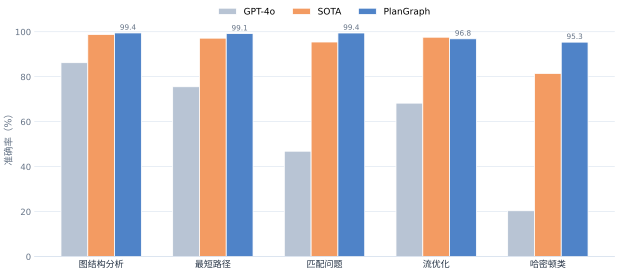
\includegraphics[width=0.94\textwidth]{figures/paper/exp_category_accuracy.pdf}
\caption{不同任务类别上的精确匹配率对比}
\label{fig:category_accuracy_comparison}
\end{figure}

由图\ref{fig:category_accuracy_comparison}可以看出，PlanGraph 在图结构分析、最短路径、匹配问题、流优化和哈密顿类五类任务上均取得了最高精确匹配率。其中，哈密顿类任务的提升幅度最明显。PlanGraph 的平均精确匹配率为 95.33\%，相比最佳现有方法的 74.30\% 高出 21.03 个百分点。该类任务通常同时涉及节点不重复访问、相邻节点连通、回路闭合以及总代价优化等要求。若直接由模型生成答案，容易出现节点遗漏、节点重复访问、路径不可行或代价计算错误等问题。PlanGraph 通过显式规划、程序执行和结果验证，将这些约束转化为可检查的步骤，因此能够更好地减少端到端生成中的结构性错误。

在流优化任务上，PlanGraph 也优于最佳现有方法。具体而言，PlanGraph 在 NLGraph-MF 和 GraphWiz-MF 两个最大流任务中均取得最优结果，两项任务的平均精确匹配率为 96.32\%，相比最佳现有方法的平均结果 94.40\% 提升 1.92 个百分点。最大流任务通常涉及残量图维护、容量更新、反向边处理和增广路径选择等实现细节，对程序实现和 API 使用都有较高要求。PlanGraph 在该类任务上的优势表明，规划生成和外部图算法知识检索能够帮助系统减少最大流求解中的实现偏差。

\subsection{复杂度与样本难度分层分析}

为考察 PlanGraph 在不同计算复杂度任务上的表现，本文将任务划分为 NP 完全任务与非 NP 完全任务两类。按照任务集合中的公开任务定义，本文将邻居查询、距离计算、连通分量和图直径等基础图任务划为非 NP 完全组，将最大独立集、最小点覆盖、最大团、图编辑距离、最大公共子图和旅行商问题划为 NP 完全组。图\ref{fig:np_complete_performance}展示了两类任务上的性能对比。

\begin{figure}[htbp]
\centering
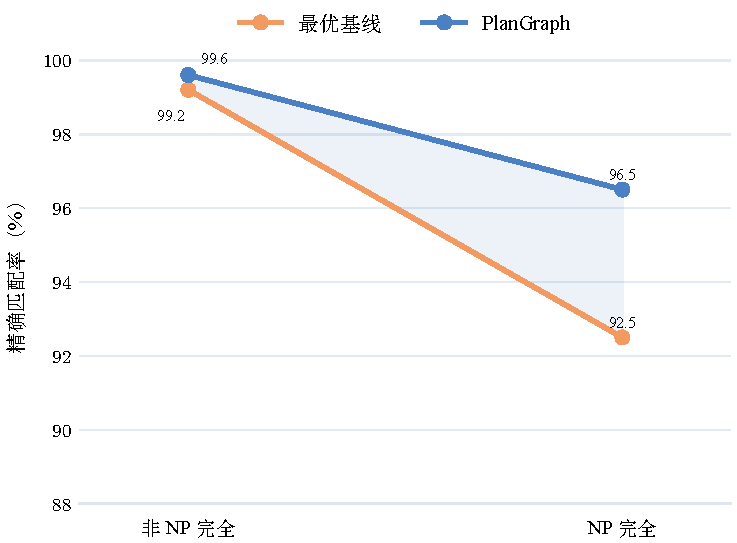
\includegraphics[width=0.86\textwidth]{figures/paper/exp_complexity_trend.pdf}
\caption{NP 完全任务性能对比}
\label{fig:np_complete_performance}
\end{figure}

可以看到，PlanGraph 在非 NP 完全任务上与最佳基线方法均达到 100.00\%，说明基础图任务已经接近饱和，提升空间有限；而在 NP 完全任务上，PlanGraph 的平均精确匹配率达到 96.23\%，较最佳基线方法的 92.87\% 提升 3.36 个百分点，说明规划与验证闭环的主要收益集中体现在高组合复杂度场景。这与最大独立集、最小点覆盖、最大团、图编辑距离、最大公共子图和旅行商问题等任务上的观察一致。

除任务复杂度外，本文还从样本难度角度观察方法表现。该划分以图规模为主要依据：简单样本对应节点数小于 15 的图实例，中等样本对应节点数为 15 至 30 的图实例，困难样本对应节点数大于 30 的图实例。图\ref{fig:sample_difficulty_performance}给出了不同难度样本上的性能对比。

\begin{figure}[htbp]
\centering
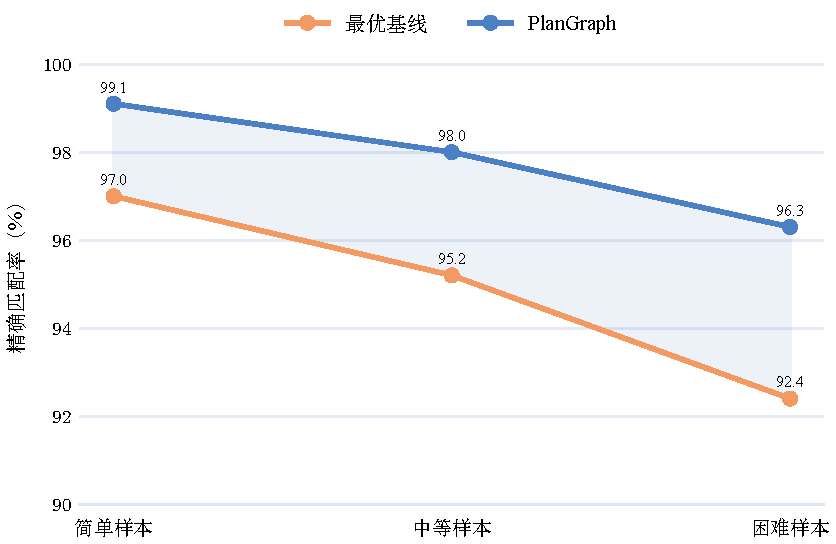
\includegraphics[width=0.86\textwidth]{figures/paper/exp_sample_difficulty_trend.pdf}
\caption{样本难度分层下性能对比}
\label{fig:sample_difficulty_performance}
\end{figure}

从图\ref{fig:sample_difficulty_performance}可见，随着样本难度提高，不同方法的性能均出现下降，但 PlanGraph 的下降幅度相对更小。尤其在困难样本上，PlanGraph 相比最佳基线方法的优势进一步扩大，说明规划先行与执行验证机制对大搜索空间下的稳定求解具有更明显作用。综合两类分层结果可以看出，PlanGraph 的性能收益主要来源于复杂任务场景，而非简单任务上的边际提升。

\subsection{各基准测试集逐任务结果}

为避免总体平均结果掩盖不同任务族之间的性能差异，本文进一步给出五个基准测试集的逐任务精确匹配率统计，以从更细粒度上分析 PlanGraph 在不同图推理场景中的适用性与性能边界。

GraphArena\cite{tang2025grapharena}是面向图计算与图推理任务的综合基准测试集，覆盖邻居查询、连通分量、最短距离、图直径、图编辑距离以及多类组合优化问题。表\ref{tab:grapharena_detail}给出了各方法在该基准测试集各子任务上的逐项结果。其中，CN、CC、SD、GD 和 GED 分别表示邻居查询、连通分量、最短距离、图直径和图编辑距离任务；MIS、MVC、MCP、MCS 和 TSP 分别表示最大独立集、最小点覆盖、最大团、最大公共子图和旅行商问题。

\begin{table}[htbp]
\centering
\caption{GraphArena 各任务精确匹配率（\%）}
\label{tab:grapharena_detail}
\begin{tabular}{lcccc}
\toprule
任务 & GPT-4o & GraphTeam & GCoder & PlanGraph \\
\midrule
CN & \textbf{100.0} & \textbf{100.0} & \textbf{100.0} & \textbf{100.0} \\
CC & \textbf{100.0} & \textbf{100.0} & \textbf{100.0} & \textbf{100.0} \\
SD & \textbf{100.0} & \textbf{100.0} & \textbf{100.0} & \textbf{100.0} \\
GD & \textbf{100.0} & \textbf{100.0} & \textbf{100.0} & \textbf{100.0} \\
GED & 23.3 & 91.0 & 89.5 & \textbf{96.5} \\
MIS & 22.4 & 97.8 & 96.8 & \textbf{98.8} \\
MVC & 19.3 & 98.6 & 97.6 & \textbf{100.0} \\
MCP & 12.5 & 90.5 & 88.7 & \textbf{100.0} \\
MCS & 8.4 & 90.8 & 89.4 & \textbf{95.3} \\
TSP & 4.9 & 82.7 & 80.7 & \textbf{86.8} \\
\bottomrule
\end{tabular}
\end{table}

表\ref{tab:grapharena_detail}显示，基础结构任务对各强基线均已较为简单，CN、CC、SD 和 GD 等子任务几乎都达到满分；图编辑距离和组合优化任务则具有较强区分度。PlanGraph 在这些高约束任务上保持更优结果，说明规划生成、知识检索和执行验证的闭环机制并非只在基础任务的饱和区间内带来边际改善，而是能够更有效地提升复杂图搜索任务中的可行性控制与错误修复能力。

NLGraph\cite{chen2024nlgraph}主要考察自然语言条件下的图算法推理能力，其核心难点不只在于调用某个图算法，而在于先从自然语言描述中恢复图结构、任务目标和求解约束，再完成相应的算法推理。表\ref{tab:nlgraph_detail}给出了各方法在 NLGraph 各子任务上的逐项结果。其中，CONN、MF、CYC、TOPO、SP、BM、HP 和 GNN 分别表示连通性、最大流、环检测、拓扑排序、最短路径、二分图匹配、哈密顿路径和 GNN 推理任务。

\begin{table}[htbp]
\centering
\caption{NLGraph 各任务精确匹配率（\%）}
\label{tab:nlgraph_detail}
\begin{tabular}{lcccc}
\toprule
任务 & GPT-4o & GraphTeam & GCoder & PlanGraph \\
\midrule
CONN & 92.10 & \textbf{100.0} & \textbf{100.0} & \textbf{100.0} \\
MF & 67.30 & 93.67 & 94.10 & \textbf{97.53} \\
CYC & 95.80 & \textbf{100.0} & \textbf{100.0} & \textbf{100.0} \\
TOPO & 60.50 & 91.20 & 92.80 & \textbf{94.80} \\
SP & 72.40 & \textbf{100.0} & \textbf{100.0} & \textbf{100.0} \\
BM & 81.30 & \textbf{100.0} & \textbf{100.0} & \textbf{100.0} \\
HP & 40.70 & \textbf{100.0} & \textbf{100.0} & \textbf{100.0} \\
GNN & 52.10 & 96.80 & \textbf{97.40} & \textbf{97.40} \\
\bottomrule
\end{tabular}
\end{table}

在 NLGraph 上，PlanGraph 对最大流和拓扑排序这类需要算法步骤清晰展开的任务提升更为明显，而在连通性、最短路径、二分匹配和哈密顿路径等已被现有方法较好解决的任务上也至少保持同等水平。该结果说明，PlanGraph 的优势主要体现在把自然语言问题稳定映射到可执行图求解过程这一环节上。

GraphWiz\cite{gong2024graphwiz}是面向指令式图推理场景构建的基准测试集，主要考察模型在给定图操作指令或明确求解要求时，能否完成任务理解、算法选择和结果输出。表\ref{tab:graphwiz_detail}给出了各方法在该基准测试集各子任务上的逐项结果。其中，CONN、CYC、BIP、TOPO、SP、MTS、MF、HP 和 SM 分别表示连通性判定、环检测、二分图判定、拓扑排序、最短路径、最大三角形权重和、最大流、哈密顿路径和子图匹配任务。

\begin{table}[htbp]
\centering
\caption{GraphWiz 各任务精确匹配率（\%）}
\label{tab:graphwiz_detail}
\begin{tabular}{lcccc}
\toprule
任务 & GPT-4o & GraphTeam & GCoder & PlanGraph \\
\midrule
CYC & 95.00 & \textbf{100.0} & \textbf{100.0} & \textbf{100.0} \\
CONN & 70.30 & 86.50 & 90.20 & \textbf{91.20} \\
BIP & 82.70 & 96.30 & 98.00 & \textbf{100.0} \\
TOPO & 75.20 & \textbf{100.0} & \textbf{100.0} & 96.50 \\
SP & 78.60 & 95.00 & 96.40 & \textbf{98.50} \\
MTS & 71.80 & 94.00 & \textbf{95.10} & 93.80 \\
MF & 69.10 & 94.00 & 94.70 & \textbf{95.10} \\
HP & 15.40 & 32.50 & 40.20 & \textbf{99.20} \\
SM & 88.30 & 99.30 & \textbf{99.50} & 98.80 \\
\bottomrule
\end{tabular}
\end{table}

GraphWiz 中差异最明显的是哈密顿路径任务，其对路径约束满足要求极高。PlanGraph 在该任务上远超对比方法，说明显式规划与程序验证对哈密顿路径类问题尤为有效。在连通性判定、最短路径和最大流等需要稳定图构建与步骤执行的任务上，PlanGraph 也保持了较强竞争力。

LLM4DyG\cite{llm4dyg2024}聚焦动态图与时间约束场景，任务通常要求模型同时处理图结构变化、时间顺序以及事件依赖关系。表\ref{tab:llm4dyg_detail}给出了各方法在 LLM4DyG 各子任务上的逐项结果。其中，WL、WC、WTC、WN、WNB、CTC、CTP、FTP 和 SE 分别表示边出现时间查询、首次连通时间查询、三元闭包形成时间查询、给定时间邻居查询、动态图邻居集合查询、三元闭包判定、时序路径判定、时序路径查找和边时间排序任务。

\begin{table}[htbp]
\centering
\small
\caption{LLM4DyG 各任务精确匹配率（\%）}
\label{tab:llm4dyg_detail}
\begin{tabular}{lccccc}
\toprule
任务 & GPT-4o & LLM4DyG & GraphTeam & GCoder & PlanGraph \\
\midrule
WL & 58.00 & 47.30 & 96.33 & 94.33 & \textbf{98.67} \\
WC & 67.33 & 64.10 & 94.33 & \textbf{94.78} & 93.56 \\
WTC & 87.67 & 63.00 & \textbf{100.00} & 97.08 & \textbf{100.00} \\
WN & 33.33 & 45.90 & 95.33 & 94.74 & \textbf{97.47} \\
WNB & 44.67 & 20.00 & \textbf{100.00} & 94.83 & \textbf{100.00} \\
CTC & 77.33 & 66.70 & 99.67 & \textbf{100.00} & 99.33 \\
CTP & 57.67 & 59.80 & 87.00 & \textbf{100.00} & 92.03 \\
FTP & 46.67 & 80.80 & 81.00 & 74.58 & \textbf{84.57} \\
SE & 49.67 & 35.80 & \textbf{99.67} & 93.67 & 99.33 \\
\bottomrule
\end{tabular}
\end{table}

从表\ref{tab:llm4dyg_detail}可以看出，PlanGraph 在边出现时间查询、给定时间邻居查询、动态图邻居集合查询和边时间排序等任务上表现较好，但在首次连通时间查询、三元闭包判定和时序路径判定等任务上尚未全面超过最优对比方法。这说明动态图任务内部差异较大。对于更依赖结构约束检查和过程验证的任务，规划反馈闭环能够带来更明显的收益；而对于需要细粒度时间建模或连续状态跟踪的任务，当前方法仍存在改进空间。

GraphInstruct\cite{graphinstruct2024}面向图指令跟随场景，强调模型能否根据任务指令稳定完成邻居查询、边判断、连通性分析、遍历与拓扑排序等基础图操作。GraphInstruct 原始设置共包含 21 个任务，本文对全部任务进行统计，不对任务集合做抽样或裁剪。表\ref{tab:graphinstruct_detail}给出了各方法在该基准测试集上的逐项结果。其中，NB、BIP、EDGE、CONN、DEG、DFS、PRED、TOPO、CC、CN、HP、JAC、SP、DIAM、PR、MF、MST、BFS、CLUST、CYC 和 EP 分别表示邻居查询、二分图判定、边存在判断、连通性、度数计算、深度优先遍历、前驱查询、拓扑排序、连通分量、公共邻居、哈密顿路径、Jaccard 系数、最短路径、图直径、PageRank、最大流、最小生成树、广度优先遍历、聚类系数、环检测和欧拉路径任务。

\begin{table}[htbp]
\centering
\small
\caption{GraphInstruct 各任务精确匹配率（\%）}
\label{tab:graphinstruct_detail}
\resizebox{\textwidth}{!}{%
\begin{tabular}{lccccc}
\toprule
任务 & GPT-4o & GraphInstruct & GraphTeam & GCoder & PlanGraph \\
\midrule
NB & 98.00 & 99.00 & \textbf{100.00} & 99.53 & \textbf{100.00} \\
BIP & 89.67 & 85.00 & 99.00 & \textbf{100.00} & \textbf{100.00} \\
EDGE & 90.67 & 84.00 & 99.33 & 97.47 & \textbf{100.00} \\
CONN & 92.22 & 83.00 & \textbf{100.00} & \textbf{100.00} & \textbf{100.00} \\
DEG & 98.00 & 81.00 & \textbf{100.00} & 98.67 & \textbf{100.00} \\
DFS & 89.33 & 46.00 & 95.67 & 94.33 & \textbf{96.33} \\
PRED & 47.41 & 41.00 & 98.00 & \textbf{99.75} & \textbf{99.75} \\
TOPO & 59.00 & 33.00 & 98.33 & \textbf{99.50} & 99.25 \\
CC & 39.30 & 83.00 & 94.67 & 83.30 & \textbf{94.74} \\
CN & 49.00 & 23.00 & \textbf{100.00} & 99.53 & 99.69 \\
HP & 33.70 & 18.00 & 97.70 & 98.75 & \textbf{99.16} \\
JAC & 17.00 & 14.00 & \textbf{100.00} & 98.91 & \textbf{100.00} \\
SP & 57.30 & 14.00 & \textbf{100.00} & \textbf{100.00} & 99.44 \\
DIAM & 23.00 & 13.00 & \textbf{100.00} & \textbf{100.00} & \textbf{100.00} \\
PR & 15.30 & 13.00 & 66.43 & 57.01 & \textbf{66.75} \\
MF & 15.00 & 6.00 & 99.30 & 93.67 & \textbf{99.67} \\
MST & 1.00 & 4.00 & 54.86 & 49.19 & \textbf{60.53} \\
BFS & 59.00 & 3.00 & 84.79 & \textbf{94.21} & 93.69 \\
CLUST & 32.00 & 9.00 & 85.06 & 84.93 & \textbf{85.38} \\
CYC & 68.00 & 71.00 & 96.46 & 95.07 & \textbf{97.96} \\
EP & 0.00 & 0.00 & 93.54 & \textbf{100.00} & \textbf{100.00} \\
\bottomrule
\end{tabular}
}
\end{table}

GraphInstruct 主要考察图指令执行能力。PlanGraph 在 21 个任务上的平均精确匹配率为 94.87\%，在 17 个任务上取得最优或并列最优，尤其在邻居查询、二分图判定、连通性、度数计算、PageRank、最小生成树、最大流和欧拉路径等任务上表现稳定，说明所提框架不仅能处理复杂求解型任务，也能处理相对基础但格式要求严格的图查询任务。

\subsection{误差归因}

结合实验过程中的失败样例，当前错误大致可以分为五类，如表\ref{tab:error_taxonomy}所示。这些错误并不只发生在代码实现阶段，也可能从规划、检索、验证或答案格式化阶段逐步累积。因此，图推理任务很难依靠单一模块完全解决，而需要中间表示、外部知识和执行约束共同发挥作用。

\begin{table}[htbp]
\centering
\small
\caption{失败样本的主要错误类型归纳}
\label{tab:error_taxonomy}
\begin{tabular}{m{3cm}m{4.5cm}m{5cm}}
\toprule
错误类型 & 具体表现 & 主要影响阶段 \\
\midrule
任务识别偏差 & 将判定任务误识别为优化任务，或混淆路径搜索与可达性判断 & 规划阶段 \\
约束遗漏 & 忽略固定起点、回路闭合、时间窗口或容量限制 & 规划/编码阶段 \\
API 误用 & 选择语义相近但并不匹配的函数，或参数使用错误 & 检索/编码阶段 \\
边界情况失效 & 在小样例上通过，但在目标图上因特殊结构而失败 & 验证阶段 \\
输出格式错误 & 路径顺序、集合表示或文本格式不符合官方脚本要求 & 答案生成阶段 \\
\bottomrule
\end{tabular}
\end{table}

从整体表现看，PlanGraph 在高约束图任务上已经展现出较强稳定性，但面对动态图、复杂时序逻辑和长尾组合搜索时仍有改进空间。后续可从时序感知规划、失败反馈驱动的知识重排序以及更具代表性的验证样例构造等方面继续完善，以提升方法在更复杂场景下的适用性。


\section{本章小结}

本章围绕基于规划反馈的图推理求解方法进行了说明。该方法先将自然语言形式的图推理任务转换为结构化任务表示，并在此基础上生成算法级伪代码规划；随后，系统利用规划结果约束外部知识检索；最后，在规划和检索知识共同约束下生成候选程序，并通过程序执行和结果检查获得反馈，据此触发局部修复、补充检索或规划重写。相比端到端直接生成答案的方式，该方法通过中间语义表示拆分任务理解、算法选择和程序实现过程，降低了一次性联合生成的难度，同时利用执行反馈及时发现并修正错误，减少错误在后续阶段中的继续传递。

本章还结合五个图推理基准测试集，从任务类别、复杂度分层、样本难度、逐任务结果和误差归因等角度验证了规划反馈式方法的有效性。实验结果表明，该方法的收益主要集中在高约束、强组合和容易出现结构性错误的图推理任务中。下一章将介绍基于黑板调度的多智能体图推理协同框架，说明上述方法如何在系统中完成调度、共享缓存管理、异常恢复和任务扩展。
      % 第三章：
\chapter{基于黑板调度的多智能体协同推理机制}
\label{chp:system}

PlanGraph 的图推理求解过程涉及规划、检索、编码、验证和反馈修复等多个阶段。第三章重点讨论规划反馈如何形成图推理求解方法，本章进一步研究多个智能体在同一求解链路中如何保持状态一致、定位错误来源并完成有界恢复。图推理通常包含结构解析、约束识别、算法选择、代码执行和答案格式化等环节，任一阶段的不稳定都可能影响最终结果；若仅依赖多个智能体自由对话，整体流程容易出现职责混杂、上下文覆盖、错误来源不清和失败后无序重试等问题。因此，本章关注的是面向多阶段图推理过程的黑板调度协同推理机制。

PlanGraph 将多智能体协作抽象为由主流程调度器、角色智能体、共享黑板和共享缓存构成的受控协同过程：主流程调度器负责阶段推进和回退决策，角色智能体负责局部任务生成，共享黑板负责维护状态和事件，共享缓存负责保存规划、检索、候选程序和验证反馈等可复核阶段结果。围绕状态一致性、错误归因和有界恢复三个目标，本章依次说明协同状态建模、协同调度、反馈恢复、运行记录诊断以及协同推理机制验证等内容。

\section{研究问题定义}

从协同推理视角看，本文关注多个角色智能体在统一控制下完成一条可追溯的图推理求解链路。给定自然语言图推理任务，PlanGraph 依次产生任务表示、规划结果、检索知识、候选程序、执行反馈和最终答案。该过程需要解决三个问题：多个智能体之间如何维护一致的共享状态，执行失败后如何判断错误更可能来自任务解析、规划约束、检索知识、程序实现还是答案格式，以及错误定位结果如何转化为局部修复、补充检索或上游回退等有界恢复动作。

因此，PlanGraph 在运行时固定三类约束：状态只通过黑板和缓存版本更新，失败只根据错误类型和剩余预算回退，实验日志必须保留阶段产物及其依赖关系。这样可以减少角色智能体在多轮协作中覆盖前序结论，也使稳定性分析和结果复核能够追溯到具体阶段。

为描述上述状态管理问题，本文将第 $t$ 个阶段的共享黑板状态抽象为：
\begin{equation}
B_t=\{Q,S,P,K,C,E,F,A\}
\end{equation}
其中，$Q$ 表示原始自然语言问题，$S$ 表示运行期结构化任务表示，与第\ref{chp:method}章中的任务描述 $T$ 对应，$P$ 表示规划结果，$K$ 表示规划引导检索得到的知识集合，$C$ 表示候选求解程序，$E$ 表示执行验证结果，$F$ 表示反馈修复信息，$A$ 表示最终答案。该抽象使多智能体协同过程可以被统一理解为围绕黑板状态 $B_t$ 的读写与转移：不同智能体只更新与自身职责相关的状态分量，主流程调度器则根据当前状态和验证反馈决定下一阶段动作。

基于上述目标，PlanGraph 将协同推理过程建模为以主流程调度器为中心、以共享黑板和共享缓存链为支撑的多智能体协同框架。PlanGraph 接收自然语言问题和图结构输入，在输出最终答案的同时，保留对应的阶段结果、运行日志和恢复记录。该设计通过明确的职责划分，把规划反馈方法落实为可控制、可记录的执行过程。

图推理任务需要在多个阶段之间稳定传递任务表示、规划、检索知识、候选程序和验证反馈。黑板调度可以集中维护共享状态，同时通过事件和缓存索引保留错误来源及恢复记录，因而更适合本文对可追踪、可恢复和可复现实验过程的要求。

\section{基于共享黑板的协同状态建模机制}

多智能体协同推理的首要问题是状态一致性。若不同角色智能体仅通过自然语言上下文传递信息，规划结果、检索知识和执行反馈容易在多轮调用中被覆盖或重新解释。为此，PlanGraph 将协同过程建模为围绕共享黑板状态的受控读写过程，通过角色智能体职责划分、黑板状态表示和事件记录约束各阶段的信息边界。

\subsection{角色智能体的职责划分}

如果让不同角色智能体仅通过自然语言彼此对话，并由模型自行决定何时规划、检索和修复，图推理流程容易出现控制流不稳定。典型问题包括角色智能体职责重复，例如规划智能体和编码智能体都重新解释任务；也包括失败后回退位置不清，例如程序执行失败后难以判断应回到规划、检索还是编码阶段。PlanGraph 因此将全局流程交由主流程调度器统一管理，各角色智能体只负责本阶段的局部任务。

图\ref{fig:system_architecture}给出了 PlanGraph 的总体架构。自上而下，系统可划分为输入与任务建模层、主流程调度层、多智能体执行层以及共享状态管理层。输入与任务建模层负责接收自然语言问题和图结构信息；主流程调度层负责推进阶段、检查状态并决定失败后的恢复动作；多智能体执行层包含问题智能体、规划智能体、检索智能体、编码智能体和推理智能体；共享状态管理层则维护黑板事件、共享缓存、知识条目和执行反馈。该架构强调运行期控制关系，即调度器如何组织各角色智能体协同、如何保存阶段状态，以及框架如何在失败后进入受控恢复路径。

\begin{figure}[htbp]
\centering

\includegraphics[width=0.98\textwidth]{figures/paper/SystemArchitecture.pdf}
\caption{PlanGraph 总体架构}
\label{fig:system_architecture}
\end{figure}

在具体运行中，调度器维护当前样例的运行状态、已有缓存项以及剩余恢复预算。各角色智能体被调用时，只读取本阶段所需的信息。例如，规划智能体读取结构化任务表示，检索智能体读取规划结果和任务标签，编码智能体读取规划与知识条目，推理智能体读取候选程序和验证反馈。阶段任务完成后，智能体将生成结果写入共享缓存，并在共享黑板中记录相应事件。角色智能体之间不直接互相调用，也不各自维护复杂的私有上下文；协作关系由调度器和黑板统一管理。

\subsection{角色智能体的读写边界}

共享黑板需要配合明确的访问边界使用。为避免多智能体协同中的职责重叠和状态覆盖，PlanGraph 为不同角色智能体和功能模块设置相对稳定的读写边界。问题智能体主要负责把原始问题写入结构化任务表示，规划智能体在此基础上写入规划和约束标签，检索智能体只根据任务表示和规划结果补充知识，编码智能体读取规划与知识生成候选程序，推理智能体则根据执行反馈修复候选程序。调度器读取黑板状态、缓存索引和错误反馈，并据此决定下一阶段动作。

\begin{table}[htbp]
\centering
\small
\caption{角色智能体读写边界}
\label{tab:agent_read_write}
\renewcommand{\arraystretch}{1.15}
\begin{tabularx}{\textwidth}{
>{\raggedright\arraybackslash}p{2.3cm}
>{\raggedright\arraybackslash}p{2.8cm}
>{\raggedright\arraybackslash}p{2.8cm}
>{\raggedright\arraybackslash}X}
\toprule
角色/模块 & 主要读取状态 & 主要写入状态 & 边界约束 \\
\midrule
问题智能体 & $Q$ & $S$ & 只负责结构化任务表示，不生成求解程序 \\
规划智能体 & $S$ & $P$ & 生成算法级规划和约束标签，不直接调用图算法 \\
检索智能体 & $S,P,F$ & $K$ & 根据规划和反馈召回知识，不改写规划内容 \\
编码智能体 & $S,P,K$ & $C$ & 根据规划和知识生成候选程序，不重新解释任务类型 \\
验证模块 & $S,P,C$ & $E$ & 执行候选程序并产生验证结果，不修复程序 \\
推理智能体 & $P,K,C,E$ & $F,C$ & 根据错误反馈局部修复，不覆盖上游缓存 \\
调度器 & $B_t,E,F$ & 阶段状态 & 决定阶段推进、回退和失败退出，不生成局部内容 \\
\bottomrule
\end{tabularx}
\end{table}

读写边界把黑板状态约束为阶段状态记录。每个角色智能体或模块只能围绕自身职责更新对应状态分量，从而减少规划被编码阶段重新解释、检索知识被修复阶段覆盖、验证反馈在多轮调用中丢失等问题。状态一致性既依赖缓存保存结果，也依赖角色智能体和功能模块对黑板状态的受控读写。

\subsection{黑板事件记录}

共享黑板在该过程中承担状态总线的作用。黑板只维护当前样例求解所需的阶段状态、缓存索引和事件摘要，使不同智能体能够围绕同一组中间结果协同工作。调度器通过 \texttt{STAGE\_STARTED}、\texttt{TASK\_PARSED}、\texttt{PLAN\_READY} 等事件编码进行同步，这些事件只记录阶段摘要、缓存索引和关键状态，不存放完整长文本内容。调度器由此可以根据事件顺序重建样例的求解过程。

\begin{table}[htbp]
\centering
\small
\caption{共享黑板中的核心事件类型}
\label{tab:blackboard_events}
\renewcommand{\arraystretch}{1.15}
\begin{tabularx}{\textwidth}{
>{\raggedright\arraybackslash}p{2.8cm}
>{\raggedright\arraybackslash}p{2.4cm}
>{\raggedright\arraybackslash}p{3.5cm}
>{\raggedright\arraybackslash}X}
\toprule
事件类型 & 触发时机 & 核心字段 & 用途 \\
\midrule
阶段启动事件 & 阶段开始 & 阶段名 & 记录调度过程并写入日志 \\
任务解析完成 & 解析完成 & 任务类型 & 为规划和检索提供任务语义 \\
规划结果就绪 & 规划完成 & 缓存编号、版本号 & 触发检索与编码阶段 \\
检索结果就绪 & 检索完成 & 检索原因、候选条数 & 为编码或修复提供知识依据 \\
候选代码就绪 & 代码生成完成 & 缓存编号、版本号 & 触发执行与验证 \\
代码失败事件 & 验证失败 & 错误码、恢复动作 & 指导调度器选择恢复路径 \\
局部修复完成 & 修复完成 & 修复轮数 & 触发再次验证 \\
结果输出完成 & 结果生成完成 & 成功标志 & 结束求解并写入最终日志 \\
\bottomrule
\end{tabularx}
\end{table}

黑板事件用于保障系统稳定运行。若缺少事件记录，调度器只能根据当前上下文判断下一步动作，容易在多轮修复后丢失失败来源。事件链可以记录当前候选程序来自哪一次规划、依赖哪一次检索、失败于哪一次验证。这种可追踪性有助于调试系统，也为本章后续关于首次通过率、修复收敛率和失败类型的分析提供了数据基础。

\section{基于错误归因的协同调度机制}

在图推理任务中，执行失败可能来自候选程序，也可能来自任务解析偏差、规划约束遗漏、检索知识不匹配或答案格式不一致。协同调度需要先判断错误来源，再选择局部修复、补充检索、重新规划或终止输出。本节将该问题建模为错误归因驱动的调度决策过程，说明调度器如何根据黑板状态、执行观测和剩余预算选择下一步动作。

\subsection{主流程调度状态转移}

为了使调度过程可解释，PlanGraph 将样例求解过程抽象为若干状态及其转移关系。表\ref{tab:scheduler_states}侧重描述调度器如何决定下一步，即当前阶段接收什么输入、产出什么结果以及失败后回到哪里。失败处理会依据失败位置和错误类型选择恢复动作，避免无条件重启。例如，规划阶段失败通常触发重新规划，检索阶段结果不足时触发补充检索，代码验证失败时则优先进入局部修复；只有当局部修复达到上限或错误类型显示当前候选不可继续利用时，系统才会触发重生成或上游回退。

\begin{table}[htbp]
\centering
\small
\caption{主流程调度器的核心状态转移}
\label{tab:scheduler_states}
\renewcommand{\arraystretch}{1.15}
\begin{tabularx}{\textwidth}{
>{\raggedright\arraybackslash}p{1.7cm}
>{\raggedright\arraybackslash}p{3.45cm}
>{\raggedright\arraybackslash}p{3.45cm}
>{\raggedright\arraybackslash}X}
\toprule
状态 & 主要输入 & 正常输出 & 失败处理 \\
\midrule
\texttt{PARSE} & 原始问题、图描述 & 任务表示 & 字段缺失时重解析；失败退出 \\
\texttt{PLAN} & 任务表示 & 规划、约束标签 & 规划为空或约束遗漏时重规划 \\
\texttt{RETRIEVE} & 规划、任务标签 & 知识条目、质量评分 & 质量低于阈值时精炼或补检 \\
\texttt{CODE} & 规划、检索知识 & 候选程序 & 代码不可执行或接口错误时修复 \\
\texttt{VERIFY} & 候选程序、验证样例 & 验证结果、错误类型 & 执行异常或错误时修复 \\
\texttt{REPAIR} & 错误反馈、候选程序 & 修复程序 & 修复后再验证；超限则回退 \\
\texttt{OUTPUT} & 验证通过结果 & 最终答案 & 格式异常时修复；失败退出 \\
\bottomrule
\end{tabularx}
\end{table}

为进一步刻画调度器的决策过程，本文将运行时状态写作
\begin{equation}
x_t=(B_t,s_t,\mathbf{b}_t)
\end{equation}
其中，$B_t$ 表示当前黑板状态，$s_t\in\mathcal{S}$ 表示当前调度阶段，$\mathbf{b}_t$ 表示各阶段剩余预算向量。执行某一阶段后，系统获得观测结果 $o_t$，其中包含阶段是否成功、错误类型、验证结果和新生成缓存索引。调度器的动作集合记为
\begin{equation}
\mathcal{U}=\{\mathrm{NEXT},\mathrm{REPAIR},\mathrm{RETRIEVE},\mathrm{REPLAN},\mathrm{REGENERATE},\mathrm{OUTPUT},\mathrm{FAIL}\}
\end{equation}
则调度策略可表示为
\begin{equation}
u_t=\pi(B_t,s_t,o_t,\mathbf{b}_t)
\end{equation}
状态转移过程为
\begin{equation}
(B_{t+1},s_{t+1},\mathbf{b}_{t+1})=\Phi(B_t,s_t,u_t,o_t)
\end{equation}
其中，$\pi(\cdot)$ 负责根据错误来源和剩余预算选择下一步动作，$\Phi(\cdot)$ 负责写入新的阶段结果、更新阶段状态并消耗对应预算。该形式化表达强调了黑板调度的两个约束：第一，调度动作必须依赖已记录的黑板状态和执行观测，避免依赖临时对话上下文；第二，恢复动作受到预算向量 $\mathbf{b}_t$ 约束，从而避免无界重试。

\subsection{错误来源分类}

在执行反馈出现后，系统需要判断失败原因并决定下一步动作。若所有失败都简单交给编码智能体重新生成程序，会导致两类问题：一是规划约束遗漏或检索知识不足无法被真正修复；二是已经正确的上游缓存会被无谓覆盖。为此，本文实现了错误来源分类，将验证反馈转化为结构化调度信号。

该分类过程的输入包括执行日志、约束验证报告和当前黑板状态，输出为错误码、错误来源、失败阶段、调度动作、回退目标、修复范围和置信度等字段。其基本决策形式可表示为：
\begin{equation}
d_t=f(B_t,V_t,L_t)
\end{equation}
其中，$B_t$ 为当前黑板状态，$V_t$ 为约束验证结果，$L_t$ 为运行日志中的错误或警告信息，$d_t$ 为调度决策。错误来源分类面向图推理任务语义进行归因，区别于底层异常名称。例如，旅行商样例中的边界逻辑错误表示程序执行本身可以完成，但回路代价计算的边界处理与闭合路径约束不一致；动态图路径样例中的约束语义错误则说明静态路径逻辑无法覆盖时间约束。

\subsection{恢复动作映射}

在获得错误来源后，调度器需要将归因结果映射为具体恢复动作。表\ref{tab:scheduler_decision_examples}给出了若干调度决策示例。对于轻量级局部错误，系统保持原规划和原检索结果不变，只修复候选程序中的局部区域；对于约束语义相关错误，系统会将错误反馈重新加入检索条件，补充任务约束或 API 用法知识；对于通过验证的样例，系统直接接受最终答案，避免额外修复轮次。

\begin{table}[htbp]
\centering
\small
\caption{错误来源分类及调度决策示例}
\label{tab:scheduler_decision_examples}
\renewcommand{\arraystretch}{1.12}
\begin{tabularx}{\textwidth}{
>{\raggedright\arraybackslash}p{2.2cm}
>{\raggedright\arraybackslash}p{3.0cm}
>{\raggedright\arraybackslash}p{2.5cm}
>{\raggedright\arraybackslash}p{2.6cm}
>{\raggedright\arraybackslash}X}
\toprule
样例 & 错误类型 & 错误来源 & 调度动作 & 修复范围 \\
\midrule
GA-TSP & 边界逻辑错误 & 编码智能体 & 局部修复 & 路径代价循环或输出格式 \\
GA-MVC & 目标最优性错误 & 编码智能体 & 精确求解后局部修复 & 算法选择与目标值计算 \\
DY-TMP& 约束语义错误 & 约束验证器 & 二次检索后局部修复 & 时间约束与算法主体 \\
NL-SP & 无错误 & 无 & 接受最终答案 & 无 \\
GA-FLOW & 无错误 & 无 & 接受最终答案 & 无 \\
\bottomrule
\end{tabularx}
\end{table}

错误来源和恢复动作之间的映射，使 PlanGraph 的调度形成带反馈分支的有界控制过程。失败发生后，调度器根据错误来源、当前黑板状态和剩余预算选择局部修复、补充检索、重新规划、重生成或失败退出。这种基于错误归因的调度方式，有助于降低无效重试并提升失败样例的可诊断性。

\subsection{有界调度策略}

错误归因给出恢复方向，预算约束进一步限制恢复深度。若系统在同一错误上无限修复，虽然表面上体现了反馈能力，实际却会造成运行成本失控和错误方向强化。PlanGraph 因此为规划尝试次数、检索尝试次数、局部修复轮数和重生成轮数分别设置上限。算法\ref{alg:blackboard_scheduler}给出了有界黑板调度过程。

\begin{algorithm}[H]
\small
\caption{有界黑板调度算法}
\label{alg:blackboard_scheduler}
\begin{algorithmic}[1]
\Require 原始图推理任务 $Q$，初始预算向量 $\mathbf{b}_0$
\Ensure 最终答案 $A$ 或结构化失败标记
\State 初始化黑板状态 $B_0 \gets \{Q\}$，当前阶段 $s_0 \gets \texttt{PARSE}$
\For{$t=0$ to $T_{\max}$}
    \State 调用阶段模块 $M_{s_t}$，获得观测 $o_t$ 与阶段输出 $z_t$
    \State 将 $z_t$、$o_t$ 写入黑板，得到更新状态 $B'_t$
    \If{$o_t$ 表示最终答案已通过验证}
        \State \Return $\mathrm{Format}(B'_t)$
    \EndIf
    \State $u_t \gets \pi(B'_t,s_t,o_t,\mathbf{b}_t)$
    \If{$u_t=\mathrm{FAIL}$}
        \State \Return 结构化失败标记
    \ElsIf{$u_t=\mathrm{REPAIR}$}
        \State $s_{t+1}\gets \texttt{REPAIR}$，消耗修复预算
    \ElsIf{$u_t=\mathrm{RETRIEVE}$}
        \State $s_{t+1}\gets \texttt{RETRIEVE}$，将错误反馈加入检索条件
    \ElsIf{$u_t=\mathrm{REPLAN}$}
        \State $s_{t+1}\gets \texttt{PLAN}$，将约束遗漏反馈加入规划条件
    \ElsIf{$u_t=\mathrm{REGENERATE}$}
        \State $s_{t+1}\gets \texttt{CODE}$，保留规划和检索缓存并重生成候选程序
    \Else
        \State $s_{t+1}\gets \mathrm{NextStage}(s_t)$
    \EndIf
    \State 根据 $u_t$ 更新预算向量 $\mathbf{b}_{t+1}$
\EndFor
\State \Return 结构化失败标记
\end{algorithmic}
\end{algorithm}

状态化调度使多智能体协作具有更清晰的职责划分。问题智能体无需了解编码阶段如何调用 NetworkX，编码智能体也无需重新判断当前任务属于哪一类图问题；各角色智能体根据调度器提供的输入完成本阶段规定的输出。PlanGraph 由统一的运行状态、事件记录和共享缓存形成稳定的执行链路，减少对智能体自由讨论的依赖。

\section{基于共享缓存的反馈恢复机制}

协同调度能够决定失败后应当进入哪一类恢复动作，但恢复动作要有效执行，还需要稳定保存阶段产物及其版本依赖。若规划、检索知识、候选程序和验证反馈只停留在临时上下文中，系统即使判断出错误来源，也难以复用正确上游状态或回放失败过程。因此，本节围绕共享缓存说明 PlanGraph 如何保存阶段结果、支撑反馈恢复，并通过版本化依赖限制无效重试。

\subsection{共享缓存链的版本管理}

在多阶段图推理系统中，状态管理需要确定中间结果的保存粒度、依赖关系以及失败后的复用方式。若所有中间内容都只保留在一次提示上下文中，上下文增长会引入无关噪声，后续智能体也可能覆盖前序结论，实验复现时还难以恢复失败前后的具体输入输出。为解决这些问题，PlanGraph 将中间结果从临时文本上下文中剥离出来，写入具有版本和依赖关系的共享缓存。

对每个样例，系统将求解过程组织为一条显式共享缓存链：
\begin{equation}
\begin{aligned}
\mathcal{M}=\{&\texttt{raw\_problem},\texttt{task\_spec},\texttt{plan},\texttt{retrieval},\texttt{candidate\_code},\\
              &\texttt{verification},\texttt{repair},\texttt{final\_answer}\}
\end{aligned}
\end{equation}
其中，\texttt{raw\_problem} 保存原始输入，\texttt{task\_spec} 保存结构化任务表示，\texttt{plan} 保存规划结果，\texttt{retrieval} 保存候选知识集合，\texttt{candidate\_code} 保存候选程序，\texttt{verification} 保存执行验证结果，\texttt{repair} 保存修复动作与修改摘要，\texttt{final\_answer} 保存最终格式化答案。共享缓存链的设计使得系统可以在不重新读取全部上下文的情况下，定位任一阶段的输入和输出。

每个缓存项都附带统一元信息，用于描述来源、版本和依赖关系。设第 $t$ 个缓存项为 $m_t$，其结构可表示为：
\begin{equation}
\begin{aligned}
m_t=(&\texttt{id},\texttt{kind},\texttt{version},\texttt{source\_module},\\
     &\texttt{timestamp},\texttt{parent\_version},\texttt{payload},\texttt{summary})
\end{aligned}
\end{equation}
表\ref{tab:artifact_fields}给出了核心字段。共享缓存以结构化对象形式保存阶段结果，可被后续阶段继续读取和消费。例如，检索智能体读取规划缓存中的任务动作、约束标签和算法族，推理智能体读取候选程序缓存和验证结果缓存。对于检索缓存，框架还会额外记录检索质量评分；当评分低于阈值时，调度器可触发知识片段精炼或查询重写后的补充检索，并将更新结果继续写入共享黑板供后续编码与恢复阶段使用。

\begin{table}[htbp]
\centering
\small
\caption{共享缓存项的核心字段}
\label{tab:artifact_fields}
\renewcommand{\arraystretch}{1.15}
\begin{tabularx}{0.78\textwidth}{
>{\raggedright\arraybackslash}p{2.8cm}
>{\raggedright\arraybackslash}X}
\toprule
字段 & 含义 \\
\midrule
\texttt{id} & 缓存项唯一标识，如 \texttt{plan:1:ad03bd12} \\
\texttt{kind} & 缓存项类别，如 \texttt{task\_spec}、\texttt{plan}、\texttt{retrieval} \\
\texttt{version} & 同类缓存项版本号，用于记录迭代过程 \\
\texttt{source\_module} & 写入该缓存项的模块名称 \\
\texttt{timestamp} & 缓存写入时间，用于记录阶段顺序 \\
\texttt{parent\_version} & 上游依赖版本，用于追踪依赖链 \\
\texttt{payload} & 缓存主体内容，如任务表示、规划或验证结果 \\
\texttt{summary} & 对长代码、长列表或复杂对象的摘要 \\
\bottomrule
\end{tabularx}
\end{table}

共享缓存链的价值可以通过旅行商问题样例加以说明。对于一个要求从固定起点出发、访问全部节点并返回起点的带权无向图任务，问题解析阶段生成的 \texttt{task\_spec} 会记录图类型、边权信息、起点约束、回路约束和输出形式；规划阶段生成的 \texttt{plan} 会记录构建带权图、固定起点、枚举候选回路、计算总代价和选择最优闭环的求解意图；检索阶段生成的 \texttt{retrieval:1} 保存与旅行商问题、哈密顿回路和路径代价计算相关的知识条目；编码阶段生成的 \texttt{candidate\_code:1} 则依赖 \texttt{plan:1} 和 \texttt{retrieval:1}。如果验证阶段发现候选程序没有正确处理回到起点的约束，PlanGraph 会保留原有缓存项，并生成 \texttt{verification:1} 和后续的 \texttt{repair:1}。这样，失败原因、修复动作和新程序版本之间形成明确依赖关系。

这种版本化管理在系统恢复中尤其重要。对于图推理任务，错误可能来自规划约束遗漏、检索知识不匹配、编码阶段遗漏边权或答案格式不符合要求等不同环节。若系统只保留最后一次生成内容，就很难判断该回到哪个阶段修复；通过缓存依赖链，调度器可以根据失败缓存项定位上游来源，并在局部修复、二次检索和重新规划之间选择合适的恢复动作。

当然，完整保存所有中间内容也会带来运行开销。因此，PlanGraph 在共享缓存管理中采用完整缓存与摘要索引相结合的折中策略。对于短文本对象，如任务标签、约束列表和错误码，系统完整保存；对于较长对象，如候选代码、检索条目列表和模型输出，系统保存完整内容的同时生成摘要，供黑板事件快速引用。当历史缓存项过多时，调度器优先保留最近轮次的完整版本，对更早版本只保留摘要、错误类型和关键依赖关系。这样既保证失败回放所需的信息不丢失，又避免将全部历史内容反复注入模型上下文。

如果不记录规划、检索和验证版本，后续稳定性、修复收敛和失败类型统计就无法追溯到具体阶段。因此，共享缓存管理既保存阶段文本结果，也保留阶段产物之间的依赖关系。

\subsection{检索反馈恢复}

规划引导检索和执行验证只有在运行期形成闭环，才能持续参与失败恢复。对于图推理任务，首次检索通常只能覆盖规划预期中的知识需求，而程序执行后暴露出的错误往往包含更具体的实现信息，例如字段缺失、API 参数不匹配、路径约束未满足或输出格式错误。若系统不能把这些失败信息重新纳入检索与修复过程，检索模块就会退化为编码前的一次性辅助工具，无法真正参与失败恢复。

为此，PlanGraph 将检索输入组织为五类查询组件：
\begin{equation}
\mathcal{Q}_{\mathrm{retr}}=\{q_{\mathrm{raw}},q_{\mathrm{task}},q_{\mathrm{plan}},q_{\mathrm{cons}},q_{\mathrm{err}}\}
\end{equation}
其中，$q_{\mathrm{raw}}$ 为原始问题文本，$q_{\mathrm{task}}$ 为结构化任务表示，$q_{\mathrm{plan}}$ 为规划伪代码，$q_{\mathrm{cons}}$ 为任务适配器给出的图类型标签与约束标签，$q_{\mathrm{err}}$ 为执行失败后的错误反馈。实际运行中，首次检索主要依赖 $q_{\mathrm{plan}}$ 与 $q_{\mathrm{cons}}$，即以规划步骤、算法提示和关键约束作为查询主线；当执行阶段暴露出新的错误信息时，框架再将 $q_{\mathrm{err}}$ 作为补充查询条件，触发面向失败原因的二次检索。

上述检索过程遵循规划锚定与反馈修正两个原则。规划锚定要求二次检索仍然围绕原始求解意图展开，避免系统因某次局部报错而偏离任务目标；反馈修正要求错误信息进入检索条件，使检索模块找到更贴近失败原因的知识条目。例如，当候选程序在旅行商任务中因图字段组织方式出错而触发 \texttt{API\_OR\_GRAPH\_ERROR} 时，二次检索会重点关注图构建、边权字段、路径代价计算等与错误直接相关的知识。

为减少语义相关但任务不匹配的检索噪声，系统在召回后执行面向任务的重排序。设候选知识条目为 $k_i$，综合得分可表示为：
\begin{equation}
\mathrm{Rank}(k_i)=
\lambda_1\mathrm{sim}_{\mathrm{task}}(k_i,T)
+\lambda_2\mathrm{sim}_{\mathrm{cons}}(k_i,\mathcal{C})
+\lambda_3\mathrm{sim}_{\mathrm{alg}}(k_i,P)
+\lambda_4\mathrm{score}_{\mathrm{snip}}(k_i)
\end{equation}
其中，$\mathrm{sim}_{\mathrm{task}}$ 表示任务类型匹配度，$\mathrm{sim}_{\mathrm{cons}}$ 表示约束标签匹配度，$\mathrm{sim}_{\mathrm{alg}}$ 表示算法族匹配度，$\mathrm{score}_{\mathrm{snip}}$ 表示条目片段自身的检索得分。该排序方式使检索模块能够结合当前规划、任务标签和失败反馈筛出更适合当前样例的知识片段。

执行验证承担将抽象规划重新压回任务约束的作用。候选程序生成后，系统会通过 \texttt{ExecutionVerifier} 在受控环境中执行程序，并将结果统一整理为包含 \texttt{ok}、\texttt{stdout}、\texttt{error\_type} 和 \texttt{stderr\_head} 等字段的验证结果。验证内容覆盖语法执行、路径合法性、总代价一致性、起止条件、组合优化可行性以及动态图时间窗口等检查。

以旅行商任务中的一次失败恢复为例，系统会先完成任务解析和规划，再依据规划结果召回相关知识并生成候选程序。若首轮验证发现程序在读取边信息时缺少必要字段，调度器会将该错误归入图构建或 API 使用问题，并选择二次检索与局部修复路径。二次检索时，系统会把错误类型和报错摘要加入查询条件；推理智能体则在不改变原始规划的前提下，重点修复图构建部分的实现逻辑。修复后的程序重新进入验证阶段，只有当路径闭合、节点覆盖和代价计算均通过检查后，系统才会进入答案输出阶段。

从运行机制看，该闭环使规划、知识和反馈能够以稳定的数据结构流动，并限制失败信息的传播范围。若候选程序只是出现 API 参数错误，系统会保留原始任务和上游规划，再依据错误类型和剩余预算选择局部修复、补充检索或上游回退，从而将反馈信号转化为可执行的恢复动作。

\subsection{执行异常恢复}

由于 PlanGraph 采用程序化求解，系统可靠性同时取决于语言模型生成质量和运行时执行控制。图推理程序可能包含组合搜索、图遍历、路径枚举或动态更新等操作，若缺少执行控制，错误程序可能出现异常退出、无限搜索、输出格式不规范或资源占用过高等问题。因此，PlanGraph 将执行控制作为系统可靠性的独立组成部分。

在执行阶段，系统对候选程序设置时间限制、标准输出捕获、异常堆栈截断和结果格式检查。时间限制用于防止组合搜索类任务进入不可接受的长尾执行；标准输出捕获用于记录程序产生的中间结果和最终答案；异常堆栈截断用于保留关键错误信息，同时避免过长报错污染后续修复上下文；结果格式检查则用于判断程序输出是否满足基准测试集要求。通过这些控制，验证结果可以同时记录程序运行状态、失败位置、局部修复适用性和上游回退需求。

本文归纳的主要错误类型及恢复路径如表\ref{tab:error_recovery}所示。表中列出的是经过系统归因后的恢复语义。语法错误和导入错误通常说明候选程序局部不可执行，但规划和检索结果未必有问题，因此优先局部修复；图构建或 API 使用错误往往说明检索知识和实际字段组织之间存在偏差，因此需要结合失败反馈进行二次检索；超时错误通常意味着当前求解路径成本过高，应优先放弃当前候选并触发重生成。

\begin{table}[htbp]
\centering
\small
\caption{主要错误类型的恢复路径}
\label{tab:error_recovery}
\renewcommand{\arraystretch}{1.15}
\begin{tabularx}{\textwidth}{
>{\raggedright\arraybackslash}p{3.4cm}
>{\raggedright\arraybackslash}X
>{\raggedright\arraybackslash}X}
\toprule
错误类型 & 典型含义 & 恢复路径 \\
\midrule
语法或导入错误 & 程序不可执行 & 保持规划与检索结果，直接局部修复 \\
空输出或约束违反 & 程序可运行，但结果不满足任务要求 & 局部修复后再次验证 \\
图构建或 API 错误 & 图字段组织或函数选择存在偏差 & 结合失败反馈二次检索，再修复 \\
答案错误 & 程序可执行，但答案与判定器不符 & 补充检索；必要时重生成程序 \\
超时错误 & 搜索开销过大或程序超时 & 终止当前执行，触发重生成 \\
上游失败或未知异常 & 规划、检索失稳或预算耗尽 & 有界回退；超预算输出结构化失败 \\
\bottomrule
\end{tabularx}
\end{table}

异常恢复机制需要保持有界。如果系统在同一错误上无限修复，虽然表面上体现了反馈能力，实际却会造成运行成本失控和错误方向强化。PlanGraph 为规划尝试次数、检索尝试次数、局部修复轮数和重生成轮数分别设置上限。设第 $s$ 个阶段的最大尝试次数为 $B_s$，当前尝试次数为 $b_s$，则调度器只在 $b_s < B_s$ 时允许继续在该阶段内修复；若达到预算上限，则根据错误类型选择上游回退、重生成或输出结构化失败结果。该预算约束在稳定性和成本之间取得平衡，避免一出错就推倒重来，也避免在错误方向上无限修补。

从机制分析角度看，异常恢复还可以支持失败归因。每次失败都会被同时记录到黑板事件和验证结果中，内容包括错误类型、触发阶段、候选程序版本、恢复动作以及恢复后的结果。借助这些记录，系统可以在当前样例中选择合适的恢复路径，也可以在实验分析中统计规划约束遗漏、API 使用错误和输出格式错误等失败类型的分布。

异常恢复机制需要同时考虑正确性、可用性和运行成本。对于组合优化任务，严格验证可能增加执行次数和反馈轮数，但能够减少表面可运行、实际不满足约束的答案；对于简单结构查询任务，系统则可以在首次验证通过后直接输出。执行控制不能保证所有失败都能被自动修复。对于核心约束已经遗漏、知识库覆盖不足或任务本身需要复杂长尾搜索的样例，局部修复可能只能缓解部分实现错误。因此，本文将异常恢复定位为提高稳定性与可诊断性的机制。

\section{基于运行记录的协同诊断机制}

黑板调度需要同时支持阶段推进和过程诊断。对于多智能体图推理任务，研究者需要知道某个样例经历了哪些阶段、失败发生在哪个版本、调度器为何选择某种恢复动作，以及最终结果是否满足任务约束。为此，本文设计运行记录诊断机制，包括黑板状态快照、约束验证反馈、协同过程复现支撑和协同过程展示。该机制将流程编排转化为可采集、可分析和可复核的运行证据。

\subsection{黑板状态快照}

黑板状态快照模块用于记录同一任务在多个智能体阶段之间的状态演化。与普通日志只记录文本输出不同，快照记录的是版本化状态对象。每当问题智能体、规划智能体、检索智能体、编码智能体、验证模块或推理智能体完成本阶段动作后，系统都会生成一个新的黑板版本，并记录该版本对应的阶段、写入模块、读取缓存、写入缓存、状态、耗时和摘要信息。设第 $t$ 个版本对应的快照记录为 $R_t$，则其可表示为：
\begin{equation}
R_t=\{I_t,O_t,\sigma_t,W_t,\Delta_t,\varepsilon_t\}
\end{equation}
其中，$I_t$ 表示该阶段读取的输入缓存集合，$O_t$ 表示写入的输出缓存集合，$\sigma_t$ 表示阶段执行状态，$W_t$ 表示写入智能体或模块，$\Delta_t$ 表示相对上一版本发生变化的字段，$\varepsilon_t$ 表示错误信息或空值。通过这种形式，黑板可以描述任务状态演化的版本序列：
\begin{equation}
\mathcal{R}=(R_0,R_1,\cdots,R_T)
\end{equation}

表\ref{tab:blackboard_snapshot_example}给出了旅行商问题样例 GA-TSP-011 的黑板快照摘要。该样例在执行验证阶段发现回路代价计算存在边界错误，随后进入反馈修复阶段并最终得到可验证答案。快照序列记录了任务经过哪些阶段、失败发生在哪个版本、由哪个模块观测到、后续修复修改了哪些缓存项。

\begin{table}[htbp]
\centering
\small
\caption{黑板状态快照的版本追踪示例}
\label{tab:blackboard_snapshot_example}
\renewcommand{\arraystretch}{1.12}
\begin{tabularx}{\textwidth}{
>{\centering\arraybackslash}p{0.8cm}
>{\raggedright\arraybackslash}p{2.4cm}
>{\raggedright\arraybackslash}p{2.2cm}
>{\raggedright\arraybackslash}p{3.2cm}
>{\raggedright\arraybackslash}X}
\toprule
版本 & 阶段 & 写入模块 & 主要输出缓存 & 状态摘要 \\
\midrule
$v_0$ & 任务解析 & 问题智能体 & 结构化任务 & 识别为带权无向闭合路径优化任务 \\
$v_1$ & 规划生成 & 规划智能体 & 规划伪代码、约束标签 & 固定起点、枚举候选路径并最小化总代价 \\
$v_2$ & 知识检索 & 检索智能体 & 候选知识 & 召回精确枚举和哈密顿回路验证知识 \\
$v_3$ & 代码生成 & 编码智能体 & 候选程序 & 生成基于排列枚举和边权查询的程序 \\
$v_4$ & 执行验证 & 验证模块 & 执行日志、验证报告 & 检测到回路代价边界计算错误 \\
$v_5$ & 反馈修复 & 推理智能体 & 修复程序、修复计划 & 将代价循环修正为闭合路径区间累加 \\
$v_6$ & 最终输出 & 调度器 & 最终答案、缓存摘要 & 提交路径 \texttt{[A,B,C,D,E,A]} \\
\bottomrule
\end{tabularx}
\end{table}

该模块的作用在于增强多智能体协同过程的可追踪性。若只保存最终答案，研究者只能知道样例是否成功，无法判断失败来自规划、检索、编码还是验证。版本化快照将每个阶段的读写关系显式化：当 $B_4$ 记录验证失败时，系统可以继续追溯其候选程序来自 $B_3$，候选程序依赖的规划和知识分别来自 $B_1$ 与 $B_2$。这种追溯关系为后续错误分类和调度决策提供了状态依据。

\subsection{约束验证反馈}

约束验证器用于判断候选程序输出是否满足图推理任务的结构性要求。仅依靠程序是否成功运行不足以保证答案正确，因为许多错误不会表现为运行异常。例如，旅行商问题可能输出一条可以打印的路径，但未访问全部节点或重复计算回路边权；最短路径任务可能输出一条存在的路径，但代价不是最短；点覆盖任务可能输出节点集合，但仍有边未被覆盖。因此，PlanGraph 在执行阶段引入任务级约束验证器，将运行成功与任务满足分开检查。

约束验证器的统一输出包括检查项、通过状态、失败原因和可读反馈。本文实验设置覆盖了通用图结构检查、输出存在性检查以及若干任务级规则。表\ref{tab:constraint_validator_rules}给出了主要规则及其作用范围。其中，\texttt{GRAPH\_SCHEMA} 和 \texttt{OUTPUT\_PRESENT} 属于通用检查，适用于所有任务；其余规则对应具体图推理任务，用于判断候选答案是否满足任务语义。

\begin{table}[htbp]
\centering
\small
\caption{图推理任务约束验证器规则}
\label{tab:constraint_validator_rules}
\renewcommand{\arraystretch}{1.12}
\begin{tabularx}{\textwidth}{
>{\raggedright\arraybackslash}p{3.3cm}
>{\raggedright\arraybackslash}p{2.8cm}
>{\raggedright\arraybackslash}X}
\toprule
规则编号 & 适用范围 & 检查内容 \\
\midrule
\texttt{GRAPH\_SCHEMA} & 全部任务 & 边端点是否存在于节点集合，图结构字段是否完整 \\
\texttt{OUTPUT\_PRESENT} & 全部任务 & 最终答案是否非空，输出是否可解析 \\
\texttt{TSP\_CYCLE} & 旅行商问题 & 路径是否闭合、是否覆盖全部节点、是否使用合法边 \\
\texttt{PATH\_FEASIBILITY} & 最短路径 & 相邻节点之间是否存在边，起止点是否符合要求 \\
\texttt{EDGE\_COVERAGE} & 点覆盖 & 返回节点集合是否覆盖图中所有边 \\
\texttt{INDEPENDENCE} & 独立集 & 所选节点两两之间是否不存在边 \\
\texttt{CLIQUE\_PAIRWISE} & 团问题 & 所选节点两两之间是否均存在边 \\
时序单调性检查 & 时序路径 & 是否存在时间见证，是否满足到达时间单调性 \\
\bottomrule
\end{tabularx}
\end{table}

在系统运行中，验证器为调度器提供外部判定信号，不替代智能体生成答案。若验证全部通过，候选程序输出可以进入最终答案阶段；若通用结构检查失败，错误通常回到任务解析或图构建环节；若任务级约束失败，则根据错误类型进入局部修复、补充检索或上游回退。表\ref{tab:constraint_validator_examples}展示了若干样例的验证统计结果。当前原型示例中每个任务均包含三类核心检查，覆盖旅行商问题、最短路径、点覆盖、独立集、团问题和时序路径查询等任务。

\begin{table}[htbp]
\centering
\small
\caption{约束验证器样例检查结果}
\label{tab:constraint_validator_examples}
\renewcommand{\arraystretch}{1.12}
\begin{tabularx}{0.88\textwidth}{
>{\raggedright\arraybackslash}p{2.3cm}
>{\raggedright\arraybackslash}p{3.1cm}
>{\centering\arraybackslash}p{1.8cm}
>{\centering\arraybackslash}p{1.8cm}
>{\raggedright\arraybackslash}X}
\toprule
样例 & 任务类型 & 检查数 & 通过率 & 主要任务规则 \\
\midrule
GA-TSP & 旅行商问题 & 3 & 100\% & 闭合回路检查 \\
NL-SP & 最短路径 & 3 & 100\% & 路径可行性检查 \\
GA-MVC & 最小点覆盖 & 3 & 100\% & 边覆盖检查 \\
GA-MIS & 最大独立集 & 3 & 100\% & 独立性检查 \\
GA-CLQ & 最大团 & 3 & 100\% & 成对连边检查 \\
DY-TMP & 时序路径查询 & 3 & 100\% & 时序单调性检查 \\
\bottomrule
\end{tabularx}
\end{table}

上述三个模块分别回答三个运行期问题：黑板快照说明样例经历了哪些阶段，错误调度记录为什么触发修复或回退，约束验证器判断输出是否满足图任务要求。这些记录为协同推理机制分析提供过程证据。

\subsection{协同过程复现支撑机制}

协同诊断还需要保证不同批次运行条件可以复现，不同任务族可以在不重写主流程的情况下接入。PlanGraph 因此将预算约束、缓存复用、运行配置和任务适配纳入统一的协同过程管理。本节说明统一配置、缓存复用和任务适配如何支撑后续实验比较和方法迁移。

\subsubsection{面向缓存复用的运行开销控制}

多智能体协同和验证反馈会引入额外的运行开销。与直接生成答案的方法相比，PlanGraph 需要依次完成任务解析、规划生成、知识检索、代码生成、执行验证以及必要的反馈修复，因此需要同时关注准确率、调用成本和执行时延。增加智能体数量或放宽修复轮数可能提高部分样例的成功率，也会推高整体运行成本。基于这一考虑，本节从开销来源、缓存优化和配置管理三个方面说明 PlanGraph 如何在保证求解质量的同时控制运行代价。

从单样例角度看，PlanGraph 的总时延可分解为：
\begin{equation}
T_{\mathrm{all}}=T_{\mathrm{parse}}+T_{\mathrm{plan}}+T_{\mathrm{retr}}+T_{\mathrm{code}}+T_{\mathrm{exec}}+T_{\mathrm{repair}}
\end{equation}
其中，$T_{\mathrm{parse}}$、$T_{\mathrm{plan}}$ 和 $T_{\mathrm{code}}$ 主要受模型调用影响，$T_{\mathrm{retr}}$ 主要受知识库检索和重排序影响，$T_{\mathrm{exec}}$ 主要受图规模和算法复杂度影响，$T_{\mathrm{repair}}$ 则是由失败样例触发的额外成本。实践中，长尾开销通常来自少数复杂样例的多轮修复和重生成。因此，系统采用局部修复优先、重生成受限、超时终止和缓存复用等策略控制运行成本。

缓存机制主要用于减少重复规划和重复检索。PlanGraph 引入 \texttt{JsonCache} 作为轻量缓存层，缓存键由结构化任务摘要、任务标签、规划版本和检索参数共同决定。对于完全相同或高度相似的任务，系统可以复用已有规划结果；对于规划和任务标签一致的检索请求，系统可以复用候选知识条目集合。系统不默认缓存最终答案，因为最终答案与具体图实例和输出格式强相关，直接复用可能破坏实验公平性。

缓存优化与黑板机制之间存在自然配合。黑板记录当前样例使用了哪些缓存项，缓存管理模块记录命中的规划或检索版本。当缓存命中时，系统仍会生成新的事件和缓存引用，并保持记录过程完整，从而避免复现实验时出现缺失步骤的问题。缓存解决的是重复计算开销问题，配置管理则进一步保证不同批次运行条件一致，因此系统还需要记录关键参数、运行产物和缓存命中情况。

\subsubsection{运行配置下的产物管理}

系统将关键运行参数显式配置化。表\ref{tab:runtime_config}给出了本文实验中使用的一组默认配置。这些配置作为主流程调度器执行各阶段时使用的约束条件，用于约束检索范围、修复深度、重生成次数和程序执行时间，不计入实验结果本身。

\begin{table}[htbp]
\centering
\small
\caption{核心运行配置}
\label{tab:runtime_config}
\begin{tabular}{m{3.0cm}m{2.0cm}m{6.1cm}}
\toprule
配置项 & 默认值 & 作用 \\
\midrule
检索返回条数 & 3 & 每次检索返回的候选知识条数 \\
最大局部修复轮数 & 1 & 单个候选程序允许的最大局部修复轮数 \\
最大重生成轮数 & 1 & 修复失败后允许的最大重生成次数 \\
最大规划尝试次数 & 2 & 规划阶段最大尝试次数 \\
最大检索尝试次数 & 2 & 检索阶段最大尝试次数 \\
单次执行超时阈值 & 15 & 单次程序执行超时阈值（秒） \\
随机种子 & 42 & 随机采样和实验复现使用的固定种子 \\
\bottomrule
\end{tabular}
\end{table}

显式配置化的意义在于约束系统行为。检索返回条数决定编码阶段可见知识范围，最大局部修复轮数决定反馈闭环深度，最大重生成轮数决定系统在失败后的探索范围，执行超时阈值决定复杂搜索的成本上限，随机种子则影响模型采样和任务处理顺序。将这些因素统一配置后，调度器才能在不同任务上保持一致的运行策略。

此外，运行结果采用统一组织方式。每个样例的原始输入、结构化任务、规划结果、检索条目、候选程序、验证反馈和最终答案均写入同一工作目录下的对应子项，缓存目录则独立保存可复用的规划与检索结果。当某个样例结果异常时，研究者可以直接检查该样例完整链路；当更换模型版本或知识库版本时，也可以通过目录和配置文件对比不同运行条件下的缓存差异。由于运行时间还会受到模型接口响应、网络环境、图规模和修复轮数等因素影响，本文重点分析开销来源及其控制机制，而不将局部运行统计外推为一般性的效率结论。

\subsubsection{面向扩展任务的适配策略}

PlanGraph 面向可迁移的图推理协同框架设计。为了让不同任务族共享规划反馈范式，框架需要通过适配器承载任务语义，并区分稳定主流程和可替换任务知识。稳定主流程包括任务解析、规划、检索、编码、验证、修复和输出等阶段；可替换任务知识则包括图类型标签、任务目标、约束集合、规划模板、知识条目和验证规则。任务适配器负责将不同图任务的语义映射到统一主流程中。

从抽象形式看，任务适配器可表示为
\begin{equation}
\mathcal{D}_{\mathrm{task}}=\{\tau,\mathcal{G}_{\mathrm{tag}},\mathcal{C},\mathcal{A}_{\mathrm{alg}},\mathcal{P}_{\mathrm{tpl}},\mathcal{V}_{\mathrm{rule}}\}
\end{equation}
其中，$\tau$ 表示任务类型，$\mathcal{G}_{\mathrm{tag}}$ 表示图结构标签，$\mathcal{C}$ 表示关键约束集合，$\mathcal{A}_{\mathrm{alg}}$ 表示候选算法族，$\mathcal{P}_{\mathrm{tpl}}$ 表示规划模板，$\mathcal{V}_{\mathrm{rule}}$ 表示验证规则集合。该形式化表示用于说明任务适配器在系统中的位置：它位于任务理解和主流程调度之间，把具体任务语义转化为后续阶段可消费的结构化条件。

任务适配器用于降低扩展新任务时对主流程调度器的侵入。若新增一个图任务，系统通常完成四类局部修改：第一，补充任务标签和约束描述，使问题智能体能够识别该任务；第二，补充规划模板，使规划智能体能够生成符合任务族特征的动作序列；第三，补充知识条目，使检索模块能够召回相关 API、算法说明和实现注意事项；第四，注册验证规则，使执行器能够检查关键约束是否满足。主流程调度器的状态转移逻辑保持不变。

以动态图最短路径任务为例，若题目要求在给定时间窗口内计算可达路径，调度器中的 \texttt{PARSE}、\texttt{PLAN}、\texttt{RETRIEVE}、\texttt{CODE} 和 \texttt{VERIFY} 等状态保持不变，任务适配器补充动态图标签、时间窗口约束、事件过滤模板以及相应验证规则。规划阶段会据此生成先筛选时间范围、再构建有效图、最后执行路径搜索的步骤序列；检索阶段会优先召回动态图处理和时间过滤相关知识；验证阶段则检查程序是否在图搜索前正确应用了时间条件。系统扩展主要体现为局部知识和规则的补充，主流程保持稳定。

这种设计使系统扩展具有配置优先、流程稳定的特点。路径类任务通常只需要调整起点、终点、边权和路径合法性约束；匹配与流类任务需要补充容量、配对关系和可行性检查；动态图任务则需要描述时间窗口、事件顺序和状态更新规则。若新任务的算法知识库覆盖不足，或验证规则难以形式化，仍可能出现规划粒度不足或验证不充分的问题。PlanGraph 的扩展性主要体现在主流程无需重写；新增任务的最终性能仍取决于知识库覆盖和验证规则质量。

从可扩展性角度看，任务适配器还便于后续替换系统组件。当知识源从文档库扩展为向量数据库、代码库或专用求解器说明时，只要保持知识条目结构一致，检索模块即可替换底层索引；当验证方式从小样例执行扩展为约束求解或静态分析时，只要保持验证结果结构一致，调度器也保持不变。PlanGraph 的可扩展性来自主流程调度、任务适配器和验证规则之间的职责分离。

\subsection{协同过程展示}

协同过程展示用于说明前述状态记录、错误诊断和约束验证结果如何被组织为可检查的运行记录。本文构建了一个面向图推理任务的交互原型，用于呈现任务解析、规划生成、规划引导检索、代码生成、执行验证和反馈修复等阶段结果。

展示原型主要呈现对话式任务输入、示例任务选择、图结构预览、答案展示和多智能体阶段结果等信息。用户可以输入最短路径、旅行商问题、连通性判断和动态图查询等任务，也可以选择若干基准风格示例任务观察系统在基础图任务、路径任务、组合优化任务和动态图任务上的执行过程。与普通对话界面不同，原型保留 Task Parsing、Pseudocode Planning、Plan-Guided Retrieval、Code Generation、Execution Verification 和 Feedback Repair 等阶段结果，使用户能够检查任务目标是否被正确识别、规划步骤是否覆盖关键约束、检索结果是否与当前任务相关、生成程序是否通过执行验证，以及反馈修复是否定位到具体错误来源。

为配合运行记录诊断机制，展示原型还在多智能体过程区域中加入 Research Modules 面板，用于集中展示黑板版本、调度决策和约束验证结果。其中，Blackboard 子面板展示各阶段快照的版本号、状态、耗时和摘要；Scheduler 子面板展示规范化错误码、调度动作、回退目标和修复范围；Validator 子面板展示任务级验证规则的通过情况和通过率。该面板在不改变主流程结构的前提下，将同一运行链路中已经产生的结构化状态进一步可视化。

原型运行服务仍遵循本文提出的主流程调度逻辑：任务解析阶段提取任务类型、图结构、起止点和约束条件；规划阶段生成算法选择、关键计算步骤和输出格式要求；检索阶段根据规划步骤召回算法说明、API 用法和约束检查规则；编码阶段生成候选程序；执行验证阶段返回标准输出、错误类型、异常摘要和约束检查结果；反馈修复阶段根据错误来源生成局部修复策略，并将修复后的程序重新送入验证流程。通过这种阶段化数据结构，原型可以将多智能体图推理过程展示为可折叠、可追踪和可复核的运行链路。

图\ref{fig:plangraph_demo_ui}展示了 PlanGraph 协同过程展示界面。示例任务采用旅行商问题，界面左侧和中间区域展示用户输入、任务信息和 PlanGraph 回答，右侧面板展示多智能体执行过程中的可检查阶段结果。该界面说明，前述黑板状态、调度决策和验证反馈可以被组织为可交互、可追踪和可复核的图推理展示原型。

\begin{figure}[htbp]
    \centering
    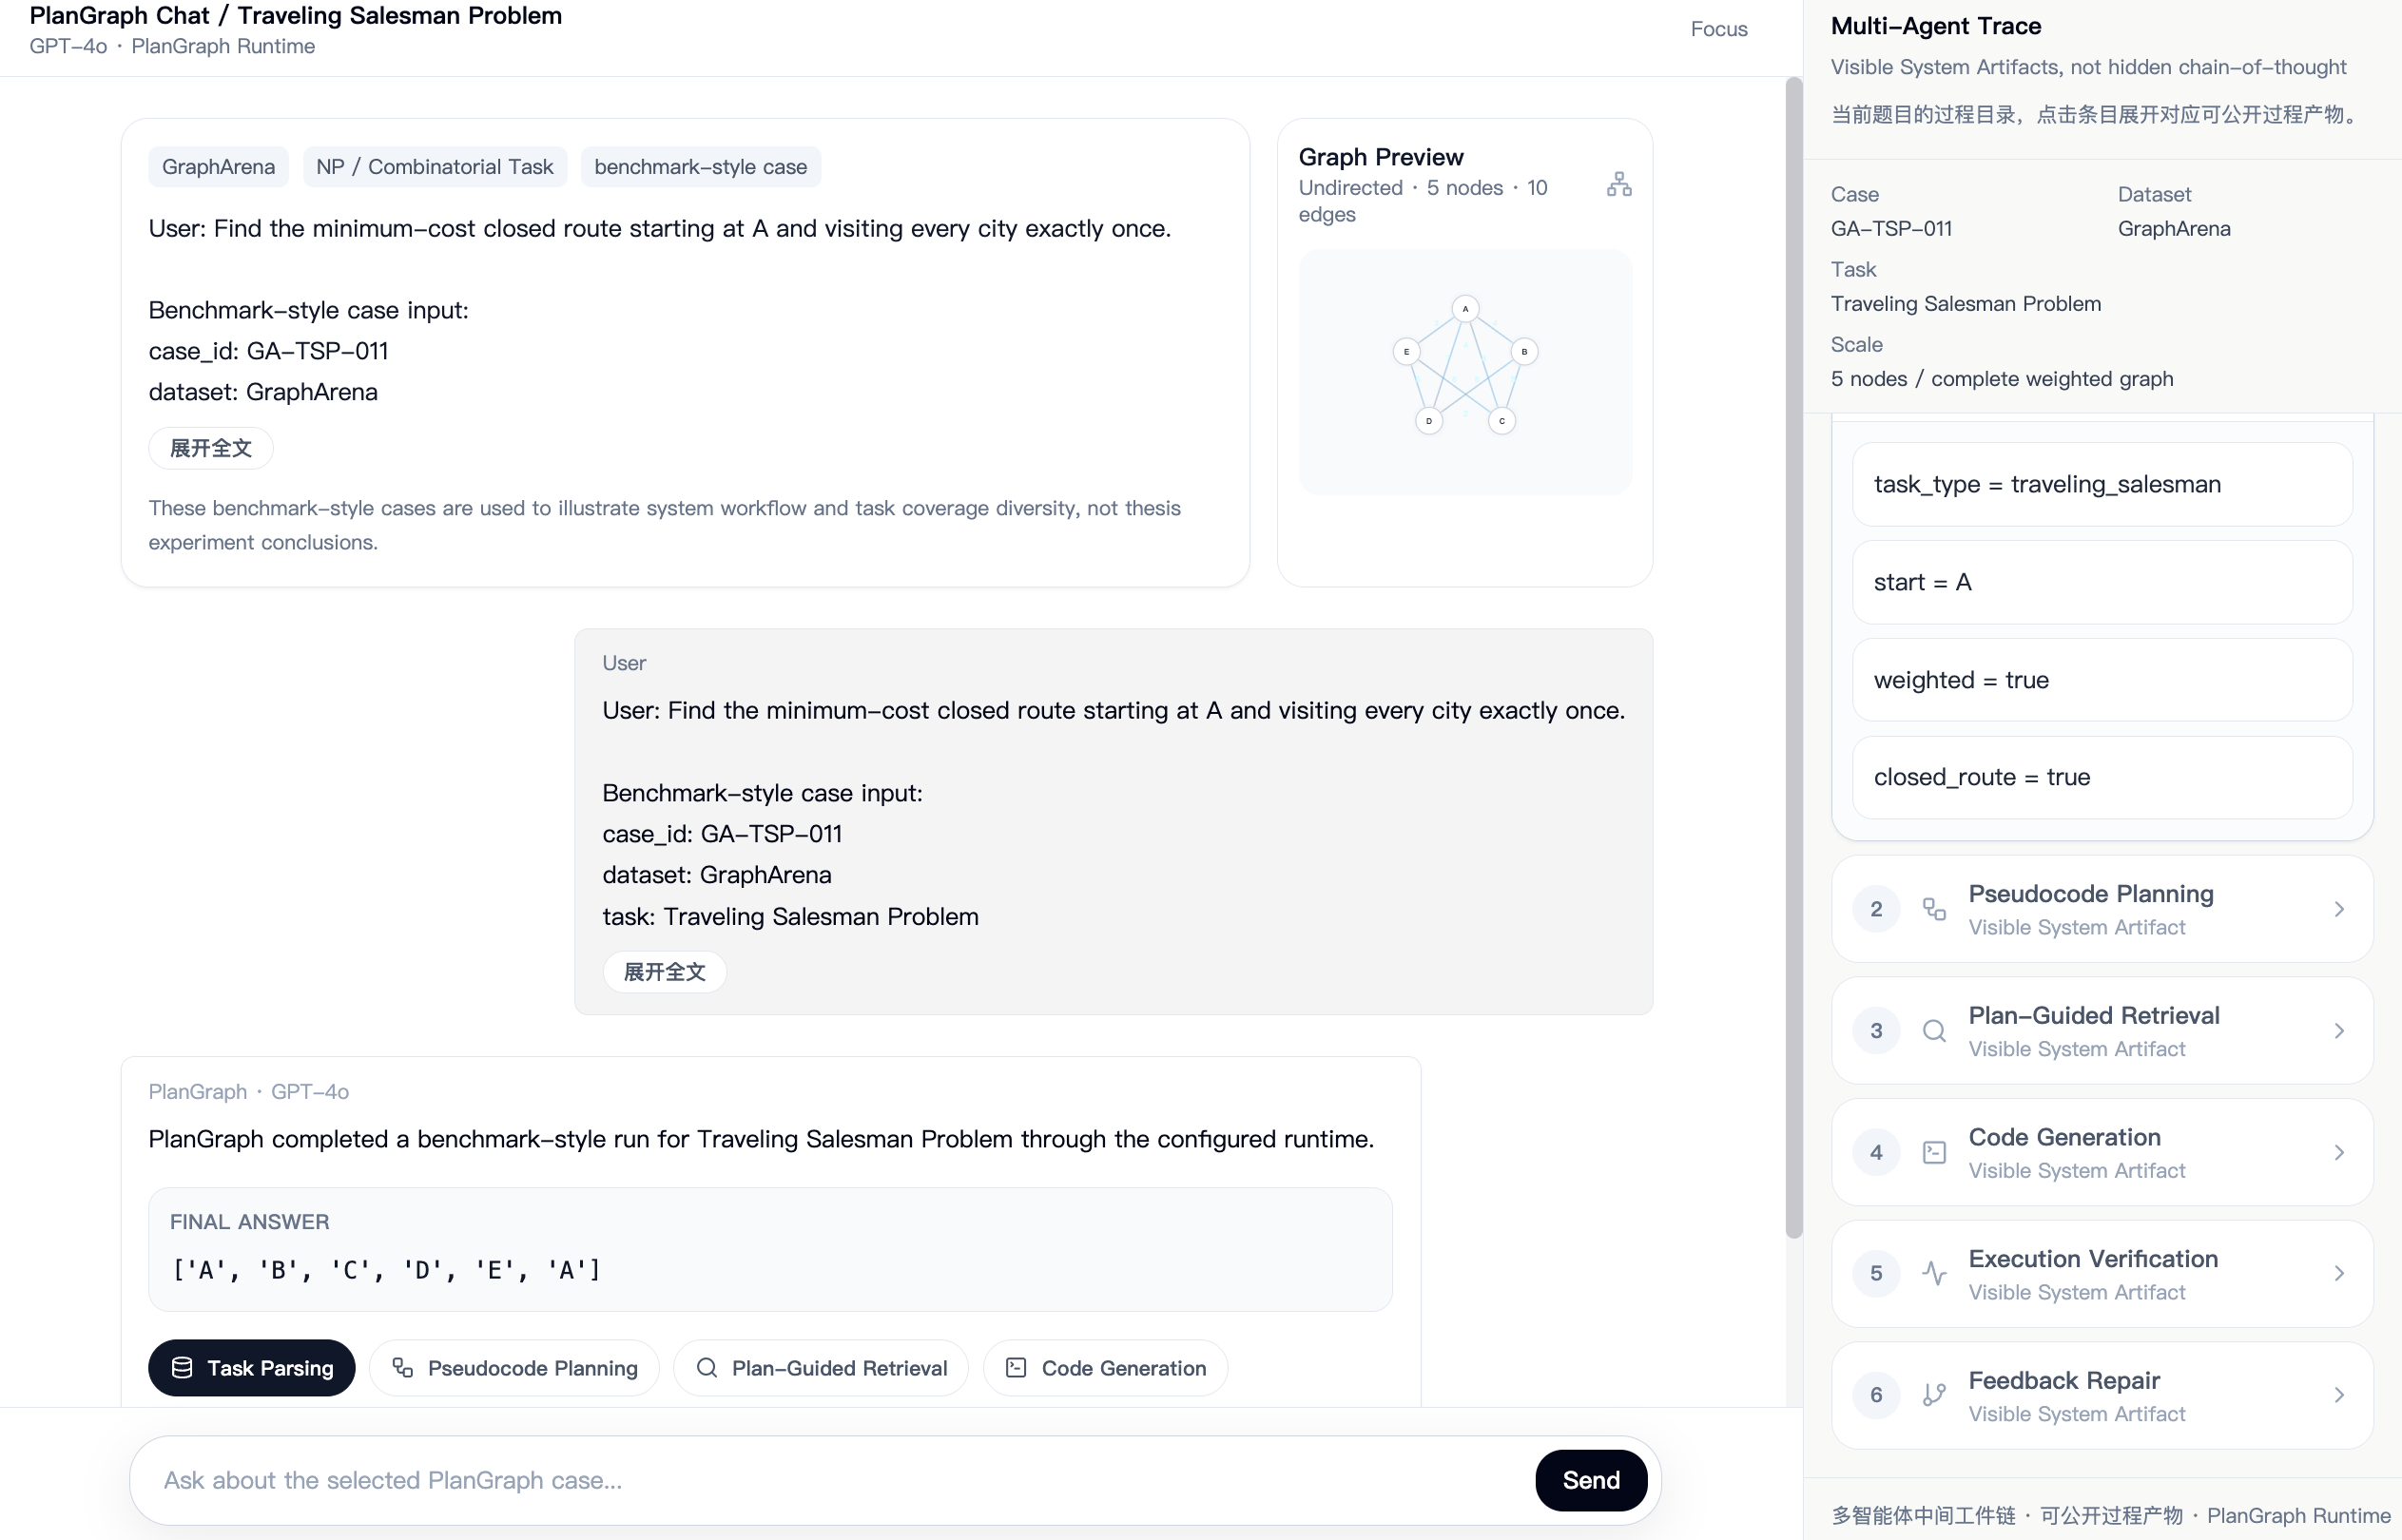
\includegraphics[width=0.95\textwidth]{figures/paper/plangraph_demo_ui.png}
    \caption{PlanGraph 协同过程展示界面}
    \label{fig:plangraph_demo_ui}
\end{figure}

展示原型仅用于呈现同一求解链路中的阶段结果，实验统计仍来自统一数据集、统一指标和批量运行日志。第四章的核心仍是黑板调度、共享缓存和反馈恢复三类机制，原型只辅助说明这些机制在单个样例中的运行过程。

\section{协同推理机制验证}
\label{sec:system_validation}

本节检验黑板调度下的协同推理机制能否稳定支撑多轮求解过程。验证重点放在三个方面：共享黑板是否能够减少状态漂移，共享缓存是否能够支撑失败回放和恢复，错误归因与预算控制是否能够降低无效重试。围绕这些问题，本文从重复运行稳定性、检索信号质量、参数预算、运行开销、鲁棒性和消融实验等方面展开验证。

\subsection{重复运行稳定性分析}

对于多智能体图推理系统而言，单次精确匹配率只能反映最终答案是否正确，还需要考察多次运行时结果是否稳定，以及候选程序在失败后能否在限定轮数内收敛。因此，本文从不同运行轮次之间的精确匹配率波动范围、程序首次生成即通过验证的比例，以及进入修复循环后能够在限定轮数内收敛的比例三个角度进行统计，结果如表\ref{tab:stability_observation}所示。

\begin{table}[htbp]
\centering
\caption{重复运行中的稳定性观察（\%）}
\label{tab:stability_observation}
\begin{tabular}{lccc}
\toprule
数据集 & 精确匹配率波动范围 & 首次通过率 & 修复后收敛率 \\
\midrule
GraphArena & $\pm0.7$ & 79.6 & 91.4 \\
NLGraph & \textbf{$\pm0.5$} & \textbf{82.3} & \textbf{93.1} \\
GraphWiz & $\pm0.9$ & 74.8 & 89.7 \\
\bottomrule
\end{tabular}
\end{table}

表\ref{tab:stability_observation}显示，结构较清晰、标准算法映射较稳定的任务在三个指标上整体更优；约束更复杂的任务首次通过率略低，但经过反馈修复后仍能保持较高收敛水平。该结果说明，PlanGraph 的协同推理机制除了提高单次运行的精确匹配率，还能抑制多次运行时的结果波动，并对失败样例提供有限恢复能力。黑板事件和共享缓存链为这些统计提供了直接依据：每次失败、修复和重新验证都被记录为可追踪事件，因此可以区分首次成功、修复成功和最终失败三类情况。

\subsection{检索质量验证}

为了更细致地验证共享黑板中的规划状态和结构约束标签是否能改善检索智能体的输入质量，本文比较四种查询方式：直接使用原始问题文本进行检索、使用任务类型和关键词进行简化检索、使用规划伪代码进行检索，以及在规划伪代码基础上补充结构约束标签进行检索。实验基于五个基准测试集构造对应查询实例，统计 Hit@1、Hit@3、Hit@5 以及平均倒数排名（MRR）四项指标，结果如表\ref{tab:retrieval_quality}所示。

\begin{table}[htbp]
\centering
\caption{不同检索查询方式的知识命中效果对比}
\label{tab:retrieval_quality}
\begin{tabular}{lcccc}
\toprule
查询方式 & Hit@1 & Hit@3 & Hit@5 & MRR \\
\midrule
Q1 原始问题文本 & 42.6\% & 61.8\% & 72.9\% & 51.4\% \\
Q2 任务类型和关键词 & 68.9\% & 84.7\% & 92.1\% & 76.3\% \\
Q3 规划伪代码 & 76.4\% & 90.8\% & 96.3\% & 83.5\% \\
Q4 规划伪代码及结构约束标签 & \textbf{82.1\%} & \textbf{94.2\%} & \textbf{98.0\%} & \textbf{88.4\%} \\
\bottomrule
\end{tabular}
\end{table}

从表\ref{tab:retrieval_quality}可见，四种查询方式呈现出清晰的层次关系：直接使用原始问题文本的效果最弱；在显式加入任务语义后，Q2 的命中效果明显提升；将问题压缩为规划伪代码后，Q3 在四项指标上继续改善；当查询中继续补充图类型、目标形式和关键约束等结构化标签时，Q4 的检索排序质量达到最好。Q3 和 Q4 在 MRR 上的提升还说明，黑板中保存的规划状态会影响正确知识的召回情况和排序位置，从而有助于减少编码阶段对错误 API 或不相关文档的尝试次数。这一结果从实验上支持了共享状态约束检索输入的协同推理机制。

\subsection{参数敏感性分析}

为观察检索返回条数和修复轮数对协同恢复过程的影响，本文比较六组代表性参数组合，即 $(1,0)$、$(3,1)$、$(5,3)$、$(7,3)$、$(5,4)$ 和 $(9,4)$。其中，$k$ 表示检索模块返回的候选知识条目数，$r$ 表示最大反馈修复轮数。该实验选取具有稳定难度分层的典型组合优化任务子集，重点比较简单样本与困难样本两个端点，并统计子集精确匹配率、难度分层精确匹配率、执行成功率、平均修复轮数与平均端到端耗时。该处数值用于分析预算约束和恢复深度，不对应第五章完整基准集合上的总体精确匹配率。

\begin{table}[htbp]
\centering
\caption{不同参数组合下典型组合优化子集的性能比较（\%）}
\label{tab:param_main_result}
\small
\resizebox{\textwidth}{!}{%
\begin{tabular}{lcccccccc}
\toprule
$(k,r)$ & 子集 EM & 简单样本 EM & 困难样本 EM & 执行成功率 & 平均修复轮数 & 平均耗时(s) & $\Delta$EM vs $(3,1)$ & $\Delta$耗时(s) vs $(3,1)$ \\
\midrule
$(1,0)$ & 70.00 & \textbf{85.00} & 55.00 & 74.20 & \textbf{0.00} & \textbf{13.80} & -4.17 & -1.40 \\
$(3,1)$ & \textbf{74.17} & 82.50 & 63.75 & 80.80 & 0.36 & 15.20 & 0.00 & 0.00 \\
$(5,3)$ & 68.75 & 75.00 & 61.25 & 78.30 & 0.92 & 18.40 & -5.42 & +3.20 \\
$(7,3)$ & 73.75 & 80.00 & \textbf{66.25} & \textbf{81.70} & 0.88 & 17.60 & -0.42 & +2.40 \\
$(5,4)$ & 71.25 & 75.00 & 65.00 & 80.40 & 1.14 & 20.90 & -2.92 & +5.70 \\
$(9,4)$ & 71.25 & 77.50 & 63.75 & 79.20 & 1.20 & 19.70 & -2.92 & +4.50 \\
\bottomrule
\end{tabular}
}
\end{table}

表\ref{tab:param_main_result}显示，$r=0$ 时 PlanGraph 缺少反馈修复能力，困难样本精确匹配率下降到 55.00\%；当参数增大到 $(7,3)$、$(5,4)$ 或 $(9,4)$ 时，更多知识条目和修复轮数未带来稳定的子集收益。相比之下，$(3,1)$ 能够在保持较高子集精确匹配率的同时控制平均修复轮数和平均耗时，说明适中的检索规模与少量反馈修复更适合作为默认配置，也说明有界恢复比无约束增加修复轮数更符合协同调度目标。

\subsection{运行开销分析}

为了说明 PlanGraph 的运行代价，本文统计了其在典型任务上的平均端到端推理耗时、平均代码生成轮数和平均验证次数。这里选取三类代表任务：最短路径、最大流和旅行商问题。平均耗时会受到模型接口响应、返回长度与验证轮次等因素影响，因此表\ref{tab:efficiency}中的数值主要用于展示本系统在不同任务之间的相对开销差异。

\begin{table}[htbp]
\centering
\caption{不同任务上的平均推理开销}
\label{tab:efficiency}
\begin{tabular}{lccc}
\toprule
任务类型 & 平均耗时（s） & 平均生成轮数 & 平均验证次数 \\
\midrule
最短路径 & \textbf{10.8} & \textbf{1.1} & \textbf{1.3} \\
最大流 & 14.6 & 1.3 & 1.8 \\
旅行商问题 & 24.3 & 1.8 & 2.7 \\
\bottomrule
\end{tabular}
\end{table}

表\ref{tab:efficiency}显示，不同任务的运行开销差异较明显。最短路径问题结构相对清楚，算法接口也较成熟，因此规划、检索和验证过程通常较为顺畅。最大流任务需要处理容量约束和残量网络，程序实现中涉及的状态更新更多，平均验证次数因此有所增加。旅行商问题还需要显式处理组合搜索、节点覆盖、回路闭合和可行性判断，因而整体耗时和验证次数最高。就本文研究目标而言，更强调可靠地完成图推理，而非追求最低时延响应，因此以一定推理开销换取更高精确匹配率和结果可信度是合理的设计选择。

\subsection{鲁棒性消融分析}

除标准基准测试集外，本文还在输入扰动设置下考察 PlanGraph 的表现，以分析框架对问题表述变化的稳定性。该实验覆盖五个基准测试集，并构造三种常见扰动：节点顺序随机打乱、边列表描述改写、输出要求从自然语言答案改为结构化列表。在相同求解任务下比较精确匹配率变化，结果如表\ref{tab:robustness}所示。

\begin{table}[htbp]
\centering
\caption{输入扰动条件下的鲁棒性分析（\%）}
\label{tab:robustness}
\begin{tabular}{lccc}
\toprule
扰动类型 & GPT-4o & GraphTeam & PlanGraph \\
\midrule
节点顺序打乱 & 51.6 & 92.4 & \textbf{96.8} \\
边描述改写 & 48.9 & 91.1 & \textbf{95.7} \\
输出格式切换 & 44.3 & 89.8 & \textbf{94.9} \\
\bottomrule
\end{tabular}
\end{table}

表\ref{tab:robustness}显示，PlanGraph 在输入扰动下仍然保持较高精确匹配率。本文认为其原因在于：问题智能体先将自然语言输入规整为结构化表示，减少了不同表述形式对后续规划的影响；程序执行结果在最终答案生成前还会经过格式化处理，因此输出形式变化对系统影响相对有限。

为判断关键协同组成是否具有必要性，本文设计三种消融变体：（1）去除规划模块，直接根据原始问题生成代码；（2）去除检索模块，移除规划引导检索，仅依赖模型内部知识生成程序；（3）去除验证模块，移除程序执行验证与反馈修复闭环，仅保留一次性代码生成。图\ref{fig:ablation_result_visual}给出了在三个代表性数据集上的消融结果。

\begin{figure}[htbp]
\centering
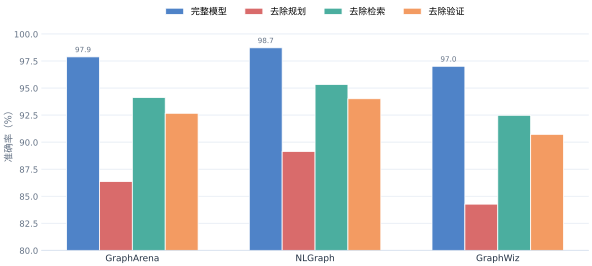
\includegraphics[width=0.90\textwidth]{figures/paper/exp_ablation.pdf}
\caption{关键协同组成消融实验结果}
\label{fig:ablation_result_visual}
\end{figure}

图\ref{fig:ablation_result_visual}显示，移除规划模块后，三个数据集上的结果都出现了最明显的下降，说明规划模块是 PlanGraph 中较关键的组成部分。去除验证模块后，系统性能也出现了较大下降，尤其在 GraphWiz 上从 97.01\% 降至 90.72\%。检索模块带来的性能提升相对温和，但依然稳定。规划模块约束任务目标与求解方向，检索模块补充实现依据，验证模块检查结果是否满足要求，三类组成形成 PlanGraph 的协同闭环。

\subsection{提示词查询模板复现说明}

为保证系统可复现性，本文将各智能体提示词和检索查询模板设计为相对固定的结构化模板。问题智能体用于将原始自然语言问题解析为结构化图推理任务，输出字段包括 \texttt{task\_type}、\texttt{nodes}、\texttt{edges}、\texttt{directed}、\texttt{weighted}、\texttt{capacity}、\texttt{params}、\texttt{output\_format} 和 \texttt{constraints}。规划智能体用于生成算法级伪代码规划，并为检索阶段提供算法提示、约束标签和检索术语。编码智能体基于任务、规划和检索知识生成可执行 Python 程序，并要求使用标准库和 NetworkX 完成图结构建模和算法调用。推理智能体则根据执行反馈和检索反馈修正当前程序，主要处理图构建错误、API 使用错误、约束遗漏和输出格式不匹配等问题。

检索智能体根据规划结果和反馈信息组织检索查询，不生成自然语言回答。其查询构造主要利用任务类型、图属性、算法提示、约束标签、输出格式以及执行错误信息。表\ref{tab:retrieval_query_template}给出了检索查询模板摘要。

\begin{table}[htbp]
\centering
\small
\caption{检索查询模板摘要}
\label{tab:retrieval_query_template}
\begin{tabular}{p{2.0cm}p{10.5cm}}
\toprule
查询类型 & 构造依据 \\
\midrule
\texttt{Q0} & \texttt{task\_type and graph attributes} \\
\texttt{Q1} & \texttt{key actions from pseudocode and algorithm\_hints} \\
\texttt{Q2} & \texttt{constraint\_tags and output\_format} \\
\texttt{Q3} & \texttt{retrieval gaps or low-coverage constraints} \\
\texttt{Q4} & \texttt{execution error type, failed API, and repair target} \\
\texttt{Ranking} & \texttt{semantic relevance, task-tag matching, and constraint consistency} \\
\bottomrule
\end{tabular}
\end{table}

上述模板避免暴露模型内部不可控推理链，并要求各阶段返回可检查的阶段结果。通过固定字段、固定查询类型和统一输出格式，PlanGraph 能够在批量实验中保持较一致的运行条件，也便于对失败样例进行回放和复核。


\section{本章小结}

本章围绕多智能体图推理中的协同推理机制展开，重点研究规划、检索、编码、验证和修复等角色如何在统一状态约束下完成一条可追踪、可恢复和可复现的求解链路。核心问题包括多个智能体如何共享状态、如何依据错误来源选择恢复动作，以及如何通过运行记录支撑机制分析。

首先，本章提出基于共享黑板的协同状态建模机制，用 $B_t=\{Q,S,P,K,C,E,F,A\}$ 描述原始问题、结构化任务、规划结果、检索知识、候选程序、执行验证、反馈修复和最终答案之间的状态关系，并通过黑板事件约束角色智能体和功能模块的读写边界。其次，本章提出基于错误归因的协同调度机制，将执行观测、错误类型和剩余预算纳入调度策略，使系统能够在局部修复、补充检索、重新规划、重生成和失败退出之间进行有依据的选择。再次，本章提出基于共享缓存的反馈恢复机制，通过缓存版本、依赖关系和运行产物管理保留阶段结果，使失败样例能够被定位、回放和复核。最后，本章通过运行记录诊断机制记录黑板快照和约束验证反馈，使协同推理过程具有可观察的研究证据。

协同推理机制验证表明，黑板事件和缓存版本能够保留阶段依赖，预算控制能够限制无效重试，反馈恢复能够提高失败样例的收敛比例。重复运行稳定性、检索信号质量、参数敏感性、运行开销、鲁棒性和消融实验进一步说明，第四章所述机制能够将多智能体协作约束为状态一致、错误可归因和恢复有边界的协同推理过程。这为后续评价完整 PlanGraph 框架的总体效果提供了运行层依据。
      % 第四章：
\chapter{综合实验验证}
\label{chp:experiment}

本章面向完整 PlanGraph 框架开展综合实验验证，重点考察其在不同图推理基准、不同任务类型和不同输入形态下的整体性能。综合实验采用统一数据集、统一评价指标和统一运行配置，对 PlanGraph 与代表性基线进行总体比较，并进一步讨论性能收益来源、系统运行特性、失败样例分布和适用边界。

\section{实验设置}

本章实验用于在统一口径下评价完整 PlanGraph 框架的整体有效性，主要回答四个问题：PlanGraph 相比现有大语言模型图推理方法是否具有整体性能优势；在不同图推理基准测试集上的表现是否稳定；复杂图任务中的收益主要体现在哪些方面；以及性能提升是否来自规划、检索、验证和黑板调度等关键机制的协同作用。为保证不同基准和不同方法之间具有可比性，本节统一说明综合实验所采用的数据集、对比基线、运行配置和评价指标，为后续总体性能结果提供一致的实验背景。

\subsection{数据集选择}

本文选取 GraphArena、NLGraph、GraphWiz、LLM4DyG 和 GraphInstruct 五个公开图推理基准测试集进行综合评估\cite{tang2025grapharena,chen2024nlgraph,gong2024graphwiz,llm4dyg2024,graphinstruct2024}。五个数据集覆盖静态图算法、自然语言图问题、指令式图操作、组合优化和动态图推理等不同场景，能够较全面地检验 PlanGraph 在多种输入形态和任务约束下的适应性。从去除数据集内部重复任务后的任务类别看，GraphArena 包含 10 类任务，NLGraph 包含 8 类任务，GraphWiz 包含 9 类任务，LLM4DyG 包含 9 类任务，GraphInstruct 包含 21 类任务。

GraphArena 侧重抽象图算法和组合优化任务，包含邻居查询、连通分量、最短距离、图直径、图编辑距离、最大独立集、最小点覆盖、最大团、最大公共子图和旅行商问题等任务，适合考察系统在标准图结构和高组合复杂度任务中的表现。NLGraph 更强调自然语言条件下的图结构恢复和算法意图识别，覆盖连通性、最大流、环检测、拓扑排序、最短路径、二分图匹配、哈密顿路径和 GNN 推理等任务。GraphWiz 面向指令式图推理，重点考察模型能否根据明确任务指令完成算法选择和过程化求解。LLM4DyG 引入时间戳、事件序列和动态图状态变化，用于检验系统处理时间边界、状态更新和时序关系的能力。GraphInstruct 覆盖 21 类图指令跟随任务，既包含邻居查询、边存在判断、度数计算等基础操作，也包含最大流、最小生成树、欧拉路径等算法化任务。

从任务层次看，上述数据集共同覆盖三类验证目标。第一类是基础结构理解，主要检验系统能否准确恢复图结构并执行基础查询；第二类是算法化求解，主要检验规划结果能否稳定映射到图算法和程序实现；第三类是强约束或高组合复杂度任务，主要检验规划、知识检索、执行验证和反馈修复能否共同减少错误传播。由于不同基准测试集在样本规模、难度划分和答案格式方面存在差异，本文在保持公开任务定义不变的前提下统一评价指标和结果统计方式，五个基准测试集均按照公开任务划分进行评测，不对任务集合做额外抽样或裁剪。

\subsection{对比基线}

本文主要与三类代表性方法进行比较。第一类是通用强基座模型 GPT-4o 的直接推理结果，用于衡量不引入显式规划、外部知识和执行反馈时，大语言模型自身完成图推理任务的能力。第二类是代表性多智能体图推理方法 GraphTeam\cite{li2024graphteam}，用于比较角色分工式多智能体协作本身是否足以支撑复杂图任务求解。第三类是代表性程序生成式图推理方法 GCoder\cite{zhang2025gcoder}，用于比较将图问题转化为代码求解这一技术路线的效果。

选择这三类基线，是因为它们分别对应当前图推理研究中的三种典型求解方式：直接提示推理、多智能体协同和程序生成求解。GraphTeam 的公开设置以 GPT-4o 作为主要语言模型；GCoder 的公开实验报告了基于 Llama3.1-8B 和 Qwen2.5-Coder 进行 LoRA 微调后的 GCoder-L 与 GCoder-Q，本文表中 GCoder 结果取二者中的较高值。PlanGraph 与这些方法的主要区别在于，它不仅将任务转化为代码，也不仅依赖多个智能体角色分工，而是在任务理解和程序执行之间引入伪代码规划层，并通过规划引导知识检索，通过执行反馈约束程序修复和必要的回退。因此，与上述基线的比较能够说明规划反馈闭环相对于直接推理、多智能体分工和单纯程序生成路线的增益。

需要说明的是，本文没有将经典图算法或 GNN 方法作为端到端对比基线。原因在于本文任务通常以自然语言问题、图结构描述和输出格式要求共同构成输入，系统需要同时完成任务解析、约束识别、算法选择、程序生成和答案格式化。经典图算法更接近 PlanGraph 内部执行器、验证器或 oracle 的组成部分，而不是同口径的自然语言图推理系统；GNN 方法则主要面向节点分类、链路预测或图表示学习等固定监督任务，也不直接覆盖本文的完整输入输出设定。

\subsection{实现配置}

实验中，PlanGraph 使用 GPT-4o 作为基础语言模型，程序执行环境统一为 Python 3.11 与 NetworkX。为降低生成随机性带来的结果波动，主实验温度参数设置为 0.2，最大输出长度设置为 2048 tokens。系统在每个样本上只保留一条最终答案，不采用多答案投票或额外采样，以避免采样策略对总体结果造成额外影响。

外部知识检索使用固定版本的轻量图算法知识库。该知识库共包含 3349 条知识条目，覆盖最短路径、最大流、最大团、最小点覆盖、最大独立集、旅行商、哈密顿路径、连通性、拓扑排序、二分图判定、图直径、邻居查询、子图匹配和最小割等常见图任务。除第四章专门讨论的参数敏感性实验外，知识库版本、检索器和重排序规则在综合实验中保持一致。

除非特别说明，本文沿用第\ref{chp:system}章给出的默认运行配置：检索返回条数设为 3，最大局部修复轮数设为 1，最大重生成轮数设为 1，规划与检索阶段的最大尝试次数分别设为 2，单次候选程序执行超时阈值设为 15 秒，随机种子固定为 42。验证样例仅用于检查候选程序是否满足基本可执行性、任务约束和输出格式，不使用目标测试样本的标准答案；最终评测仍以公开数据集的标准答案和统一评测脚本为准。

\subsection{评价指标}

为确保不同基准测试集间结果可比较，本文在主实验中统一采用精确匹配率（Exact Match, EM）作为总体性能指标。设测试集样本数为 $N$，其中模型完全答对的样本数为 $N_c$，则精确匹配率定义为：

\begin{equation}
\mathrm{EM} = \frac{N_c}{N} \times 100\%
\end{equation}

对于代码生成类方法，精确匹配率按完全匹配口径统计。所有失败样例均保留在统计中，包括运行错误、超时错误、输出不可解析的格式错误以及程序运行成功但答案错误的情形，不进行人工过滤或事后修正。

除 EM 外，本文还在第三章和第四章使用 Hit@k、MRR、首次通过率、修复后收敛率、执行成功率、平均修复轮数和平均耗时等辅助指标。这些指标不替代总体精确匹配率，而是用于解释性能来源和系统运行特性。其中，检索质量验证使用 Hit@k 与平均倒数排名（MRR），用于衡量不同查询方式对知识命中与排序质量的影响。若第 $i$ 个查询的正确知识条目排序位置为 $\mathrm{rank}_i$，则：

\begin{equation}
\mathrm{Hit@}k = \frac{1}{N}\sum_{i=1}^{N}\mathbb{I}(\mathrm{rank}_i \le k)\times 100\%
\end{equation}

\begin{equation}
\mathrm{MRR} = \frac{1}{N}\sum_{i=1}^{N}\frac{1}{\mathrm{rank}_i}\times 100\%
\end{equation}

执行成功率用于衡量候选程序是否能够正常执行并返回可解析、可验证的结果，平均修复轮数与平均端到端耗时分别用于刻画反馈修复成本和运行代价。设可成功完成代码执行并返回可验证结果的样本数为 $N_s$，第 $i$ 个样本触发的修复轮数为 $r_i$，端到端耗时为 $t_i$，则：

\begin{equation}
\mathrm{ExecSuccess} = \frac{N_s}{N}\times 100\%
\end{equation}

\begin{equation}
\mathrm{AvgRepair} = \frac{1}{N}\sum_{i=1}^{N} r_i
\end{equation}

\begin{equation}
\mathrm{AvgTime} = \frac{1}{N}\sum_{i=1}^{N} t_i
\end{equation}

上述分项指标用于解释总体精确匹配率背后的机制来源，其中 Hit@k 与 MRR 反映检索质量，执行成功率和平均修复轮数反映反馈闭环的稳定性，平均耗时则反映完整框架的运行代价。

\section{总体性能结果}

表\ref{tab:overall_result}给出了 PlanGraph 在统一评测集合上的总体精确匹配率结果，其中任务数表示本文实际纳入主实验统计的任务类别数量。PlanGraph 在五个基准测试集中有四个取得最优结果，在其余一个基准测试集上保持竞争力，平均精确匹配率达到 96.89\%，相比最佳现有方法平均提升 2.31 个百分点。

\begin{table}[htbp]
\centering
\small
\caption{不同基准测试集上的总体精确匹配率对比（\%）}
\label{tab:overall_result}
\begin{tabular}{lcccccc}
\toprule
基准测试集 & 任务数 & GPT-4o & GraphTeam & GCoder & PlanGraph & 提升幅度 \\
\midrule
GraphArena & 10 & 49.08 & 95.14 & 94.27 & \textbf{97.74} & +2.60 \\
NLGraph & 8 & 51.40 & 97.71 & 96.90 & \textbf{98.72} & +1.01 \\
GraphWiz & 9 & 47.61 & 88.62 & 90.20 & \textbf{97.01} & +6.81 \\
LLM4DyG & 9 & 58.04 & \textbf{96.35} & 93.78 & 96.11 & -0.24 \\
GraphInstruct & 21 & 51.14 & 93.48 & 92.56 & \textbf{94.87} & +1.39 \\
\midrule
平均 & -- & 51.45 & 94.26 & 93.54 & \textbf{96.89} & +2.31 \\
\bottomrule
\end{tabular}
\end{table}

从具体结果看，PlanGraph 在 GraphWiz 上提升最为明显，较 GCoder 提升 6.81 个百分点。这意味着在算法约束较强、路径搜索更复杂的任务中，规划反馈闭环能够较明显地减少直接生成带来的错误。PlanGraph 在 GraphArena 和 NLGraph 上也取得了稳定提升，反映出本文方法对经典图算法和自然语言图问题都具备较强适配性。

在 GraphArena 上，PlanGraph 的总体精确匹配率为 97.74\%，相比 GraphTeam 和 GCoder 均有提升。该数据集同时包含基础图结构任务和组合优化任务。基础任务已经接近饱和，各方法差距较小；真正拉开差距的是图编辑距离、最大独立集、最小点覆盖、最大团、最大公共子图和旅行商问题等复杂任务。对于这类任务，模型需要同时维护候选解可行性和目标函数最优性，直接推理或一次性代码生成容易遗漏关键约束。PlanGraph 在该数据集上的提升说明，显式规划和执行验证能够在组合优化场景中发挥较稳定作用。

在 NLGraph 上，PlanGraph 取得 98.72\% 的总体精确匹配率，较最佳现有方法提升 1.01 个百分点。该数据集更强调自然语言条件下的图算法推理，任务输入往往需要先从文本中恢复图关系、任务目标和输出形式。PlanGraph 的优势在于问题智能体和规划智能体先将自然语言描述转换为结构化任务表示和算法级规划，再进入检索与编码阶段。该流程降低了自然语言表述变化对后续程序生成的影响，也使最大流、拓扑排序等依赖明确步骤的任务更容易得到稳定求解。

在 GraphWiz 上，PlanGraph 的提升最为明显，达到 97.01\%。该数据集中的哈密顿路径、最大流、最短路径和子图匹配等任务对算法步骤和输出规范要求较高。尤其是哈密顿路径类问题，若没有显式约束检查，模型常会输出看似合理但不满足路径覆盖或节点不重复要求的答案。PlanGraph 通过规划阶段显式列出路径约束，并在验证阶段检查候选程序输出是否满足这些约束，因此能够显著降低结构性错误。

在 LLM4DyG 上，PlanGraph 与最佳方法相差 0.24 个百分点，结果略低于 GraphTeam，但整体仍具有竞争力。造成这一现象的原因主要在于，LLM4DyG 不只考察静态拓扑关系，还要求模型在事件序列中处理时间边界、状态更新和关系首次成立等条件。GraphTeam 的知识库包含历史经验信息，因此在部分动态图任务上可以利用相似任务的经验解法。相比之下，PlanGraph 当前主要依赖通用 Python 图计算函数 API 与算法文档，不预先构建面向各类任务的人类专家答案或历史经验库。因而，PlanGraph 在 LLM4DyG 上略低于 GraphTeam 的同时，也说明本文方法是在较轻知识先验条件下取得了接近最优的结果，具有较低的知识构建成本和更好的跨任务适配潜力。

在 GraphInstruct 上，PlanGraph 的总体精确匹配率为 94.87\%，优于 GraphTeam 和 GCoder。该数据集的特点是任务类别较多，且许多任务表面上属于基础图操作，但输出格式和指令跟随要求较严格。PlanGraph 在邻居查询、边存在判断、连通性、度数计算、PageRank、最大流、最小生成树和欧拉路径等任务上表现稳定，说明本文方法不只适用于高复杂度组合优化任务，也能够通过结构化解析和输出格式约束提高基础图指令任务的稳健性。少数任务如 BFS、拓扑排序和公共邻居等仍存在轻微差距，主要与输出顺序、并列解表示和格式严格匹配有关。

从不同基线的表现差异来看，GPT-4o 直接推理在各个基准测试集上均明显低于程序生成式方法和多智能体方法，说明图推理任务较依赖外部结构化求解能力。GraphTeam 和 GCoder 已经取得较高性能，而 PlanGraph 除 LLM4DyG 外仍能在其余四个基准测试集上继续提升结果，表明仅依赖多智能体分工或代码生成并不充分。对于复杂图任务，规划、知识检索和执行验证之间是否形成有效配合，同样会影响最终求解质量。

进一步看，PlanGraph 的提升幅度在不同数据集之间并不完全一致。这种差异与各数据集的任务构成有关：当任务包含更多显式约束、搜索空间较大或容易出现程序实现偏差时，规划反馈闭环的收益更明显；当任务主要是基础结构查询或已有方法已经接近满分时，PlanGraph 的提升空间相对有限；当任务需要细粒度时序状态建模时，当前方法虽然保持竞争力，但仍可能受到规划粒度和验证样例覆盖不足的限制。这一结果与第\ref{chp:method}章的复杂度分层分析和第\ref{chp:system}章的协同推理机制验证能够相互印证。

\section{性能收益来源分析}

总体性能结果说明了 PlanGraph 在统一评测口径下的整体优势，但平均精确匹配率本身并不能充分解释性能提升来自哪些机制。为进一步分析收益来源，本文将实验结果与方法机制、协同推理机制和完整框架三个层面的验证目标对应起来，如表\ref{tab:experiment_mapping}所示。

\begin{table}[htbp]
\centering
\small
\caption{综合实验组织与验证目标}
\label{tab:experiment_mapping}
\begin{tabularx}{\textwidth}{p{3.2cm}p{3.0cm}X}
\toprule
实验内容 & 验证层面 & 验证目标 \\
\midrule
任务类别、NP 完全和样本难度分层分析 & 方法层 & 验证规划反馈方法在复杂、高约束图任务中的收益来源 \\
逐任务结果分析 & 方法层 & 展示方法在不同任务族中的具体表现和错误边界 \\
检索质量验证 & 协同机制层 & 验证规划引导检索与结构约束标签对知识命中效果的提升 \\
稳定性、参数敏感性与运行开销 & 协同机制层 & 验证黑板调度、反馈恢复和运行配置是否支撑稳定运行 \\
鲁棒性与消融实验 & 框架层 & 验证关键模块必要性以及输入扰动下的运行稳定性 \\
总体性能对比 & 综合层 & 在统一实验口径下综合评价 PlanGraph 的整体有效性 \\
\bottomrule
\end{tabularx}
\end{table}

从表\ref{tab:experiment_mapping}可以看出，PlanGraph 的性能收益并非来自单一组件，而是来自方法层、协同机制层和框架层之间的协同。方法层实验主要说明规划反馈是否能够改善复杂图任务的求解质量；协同机制层实验主要说明多智能体协同、黑板调度、共享缓存管理和反馈恢复是否能够支撑方法稳定运行；综合层实验则在统一评价口径下检验完整框架相对于代表性基线的整体表现。

从方法层看，规划反馈的收益并不是均匀分布在所有任务上。任务类别分析说明 PlanGraph 并非只在某一类任务上偶然有效；NP 完全任务和困难样本分析说明其收益主要集中在高约束、高组合复杂度场景；逐任务结果则展示了不同数据集内部的细粒度差异。由此可以看出，规划反馈机制主要在需要显式约束维护、算法步骤拆解和执行结果校验的任务中发挥作用。

从协同机制层看，方法收益能否稳定转化为最终性能，还取决于黑板调度和反馈恢复是否能够稳定运行。重复运行稳定性对应黑板事件和共享缓存链能否抑制多轮协作中的状态漂移；检索质量对应规划引导查询是否真正改善知识命中；参数敏感性和运行开销对应调度预算是否合理；消融实验则对应规划、检索和验证模块是否具有不可替代性。这些实验共同说明，协同推理机制不是方法之外的附属实现，而是保证 PlanGraph 可追踪、可恢复和可复现的必要条件。

从完整框架看，PlanGraph 的总体表现可以理解为“规划反馈带来的求解质量提升”和“黑板调度带来的运行稳定性”共同作用的结果。前者解释复杂图任务上为什么能够减少约束遗漏和算法选择错误，后者解释多阶段求解过程为什么能够被记录、修复和复核。因此，本章的总体性能结果不是孤立的数值汇总，而是对前述方法机制和协同推理机制的统一检验。

\section{典型案例分析}

为了更直观地说明 PlanGraph 的工作过程，本文选取 GraphArena 中一个旅行商问题样例进行分析。该样例给定一个五节点带权无向图，要求从节点 A 出发，访问所有节点恰好一次并返回起点，同时使路径总代价最小。

\begin{figure}[htbp]
\centering

\includegraphics[width=0.95\textwidth]{figures/paper/case2.pdf}
\caption{案例求解流程图}
\label{fig:tsp_case_pipeline}
\end{figure}

常见错误主要包括：未访问全部节点，生成的路径并非哈密顿回路；节点出现重复访问，违反每个节点只访问一次的约束；虽然路径形式正确，但代价计算错误；以及混淆无向边和有向边，导致路径不可达。这些错误的根本原因在于，模型很难在一次生成中同时兼顾图构建、约束检查、路径枚举和最优性判定。

PlanGraph 对该任务的求解意图可以概括为：构建带权无向图，固定起点 A，枚举满足哈密顿回路约束的候选路径，计算每条路径总代价，选择总代价最小的回路并格式化输出。在此基础上，系统会围绕路径搜索、组合遍历和图构建等关键点补充相应知识，并通过测试样例检查是否恰好访问全部节点、是否回到起点、是否按权重正确计算代价以及输出格式是否符合要求。若某次生成的候选程序遗漏返回起点这一约束，验证阶段可以通过测试样例及时发现该问题，并将错误反馈给修复阶段。经过修正后，系统输出的最优路径为
\begin{equation}
A \rightarrow B \rightarrow E \rightarrow D \rightarrow C \rightarrow A
\end{equation}
对应总代价为 18。

\section{失败样例分析}

虽然 PlanGraph 在多个基准测试集上取得了较高精确匹配率，但仍然存在失败样例。对这些失败样例进行分析，可以进一步说明完整框架的适用边界，也能解释为什么某些数据集或任务类别上的提升幅度有限。结合方法层误差归因和协同过程运行日志，失败样例的主要来源可归纳为六类，如表\ref{tab:failure_summary_ch5}所示。

\begin{table}[htbp]
\centering
\small
\caption{失败样例来源与改进方向总结}
\label{tab:failure_summary_ch5}
\begin{tabularx}{\textwidth}{p{2.6cm}p{4.1cm}p{3.4cm}X}
\toprule
失败来源 & 典型表现 & 影响任务 & 改进方向 \\
\midrule
任务解析偏差 & 从自然语言中抽取的图结构、起终点或任务类型不完整 & 场景化路径任务、动态图查询 & 增强结构化解析约束，引入字段完整性检查 \\
规划粒度不足 & 规划只给出泛化步骤，未展开时间过滤、闭环约束或边界条件 & 动态图、旅行商、哈密顿路径 & 细化任务族规划模板，增加约束标签 \\
知识检索不匹配 & 检索结果语义相关但 API 输入输出或适用图类型不一致 & 最大流、匹配、子图任务 & 加强任务标签过滤和失败反馈重排序 \\
候选程序实现错误 & 参数名、边权字段、容量字段或返回值处理错误 & 最短路径、最大流、组合优化任务 & 利用执行反馈进行局部修复和补充检索 \\
验证覆盖不足 & 小样例通过，但目标样例存在特殊结构或边界情况 & 大规模图、长尾任务 & 自动生成更多边界验证样例 \\
输出格式不一致 & 答案内容正确但列表顺序、大小写或文本格式不匹配 & GraphInstruct、NLGraph & 增加格式约束和评测脚本对齐检查 \\
\bottomrule
\end{tabularx}
\end{table}

第一类失败主要来自任务解析偏差。在自然语言输入较长、边关系描述较分散或任务目标隐含在背景语句中时，问题智能体可能未能完整抽取节点集合、边集合、起点终点或关键约束。此类错误一旦发生，后续规划和程序生成都会建立在不完整的任务表示上，即使代码能够正常执行，最终答案仍可能偏离题意。对于这类问题，单纯增加修复轮数并不一定有效，更合理的方向是在解析阶段引入字段完整性检查，并在缺失关键字段时触发重新解析或要求规划阶段显式确认输入条件。

第二类失败来自规划粒度不足。这类错误在动态图和组合优化任务中较为典型。例如，动态图任务需要先根据时间窗口过滤事件，再构建有效图并执行查询；旅行商和哈密顿路径任务则需要显式检查节点覆盖、路径连通和回路闭合。如果规划只写成“求解最优路径”或“判断动态图关系”这类泛化描述，编码阶段就容易遗漏真正决定答案正确性的边界条件。该现象说明规划不应只是自然语言解释，而应具有足够清晰的算法动作和约束标签。

第三类失败与知识检索不匹配有关。图算法库中有些 API 的功能描述相近，但适用条件、参数名称和返回值形式并不完全相同。例如，最短路径、路径长度、所有简单路径和加权路径搜索都与路径任务相关，但它们的输入参数和输出结构不同；最大流任务中也存在流值、流字典、容量字段和残量网络等多个相关概念。若检索结果只在语义上相关，却没有与当前任务的图类型和约束形式对齐，编码智能体就可能选择错误接口。第\ref{chp:system}章的检索质量实验已经表明，加入规划伪代码和结构约束标签能够显著改善这一问题，但在长尾任务上仍有继续优化空间。

第四类失败来自候选程序实现错误。这类错误包括变量名不一致、边权字段读取错误、容量字段缺失、返回值解析错误和格式化输出异常等。与规划错误不同，实现错误通常可以通过执行反馈定位，因此 PlanGraph 的局部修复机制对这类失败具有较好恢复能力。表\ref{tab:stability_observation}中的修复后收敛率也说明，多数实现层错误能够在有限轮数内被纠正。剩余问题主要出现在错误同时涉及多个位置，或候选程序整体结构与规划不一致的情况，此时局部修复可能不如有界重生成有效。

第五类失败与验证覆盖不足有关。执行验证可以发现大量约束违反和运行错误，但验证样例不可能覆盖所有边界情况。若验证样例规模过小或结构过于简单，候选程序可能在小样例上通过，却在目标图上因特殊结构失败。例如，路径任务中目标图可能存在断边、重复边或不可达节点；组合优化任务中目标图规模增大后可能触发搜索超时；动态图任务中某些事件边界只有在特定时间点才会暴露错误。因此，验证样例生成质量直接影响反馈修复的效果。

第六类失败来自输出格式不一致。精确匹配评测通常对答案格式较敏感，即使系统已经计算出正确结果，如果最终输出包含多余自然语言、列表顺序不符合要求、大小写不一致或集合表示方式不同，也可能被判为失败。GraphInstruct 和 NLGraph 中部分基础图任务的差距主要与这一问题相关。该类错误并不表示系统缺乏图推理能力，但会影响最终评测结果。因此，后续可进一步加强输出格式模板和评测脚本对齐，使答案生成阶段更加稳定。

总体来看，失败样例并非集中在单一模块，而是分布在解析、规划、检索、编码、验证和输出多个阶段。这也从反面说明，图推理任务需要一个可追踪的多阶段求解框架。如果系统只输出最终答案，就很难判断失败原因；而 PlanGraph 保存的任务表示、规划、检索结果、候选代码、验证反馈和修复记录，使研究者可以将错误定位到相对明确的阶段。上述分析也提示后续改进方向应集中在三个方面：提高规划表示的约束粒度，提高检索结果与任务条件的匹配程度，以及提高验证样例对边界条件的覆盖能力。

\section{综合结果讨论}

综合前述实验结果，可以得到三个主要结论。第一，PlanGraph 的性能提升主要来自复杂图任务场景，而不是简单结构查询任务上的边际收益。在非 NP 完全任务和简单样本上，不同强方法之间差距较小；当任务进入 NP 完全或困难样本区间后，规划、检索与验证模块的协同作用更加明显。第二，PlanGraph 的优势并不只来自代码生成能力，而是来自任务解析、规划生成、知识检索、程序执行和反馈修复之间的闭环协作。消融实验显示，移除规划模块、检索模块或验证模块都会造成性能下降，其中规划和验证对结果影响尤为明显。第三，协同推理机制对方法稳定落地具有必要性。黑板事件、缓存版本、调度状态和配置管理使得多智能体协作过程可以被追踪、复现和恢复，避免系统退化为无序的多轮自由对话。

从方法层面看，PlanGraph 的核心作用可以概括为将图推理任务从一次性生成问题转化为分阶段约束求解问题。任务解析阶段降低自然语言输入的不确定性，规划阶段明确算法路线和关键约束，检索阶段补充外部图算法知识，编码阶段将规划转化为可执行程序，验证阶段检查程序是否满足任务条件，反馈阶段则根据错误类型选择局部修复、补充检索或重新规划。由于每一阶段都有明确输入和输出，系统能够避免在单一上下文中同时处理所有目标，从而降低复杂任务中的错误耦合。

从运行机制看，PlanGraph 的关键并不是简单设置多个智能体，而是通过黑板调度将多个智能体组织为可控流程。多智能体自由对话虽然灵活，但容易出现角色职责重叠、上下文覆盖和失败后无序重试等问题。本文的黑板调度通过状态转移、事件记录和缓存版本管理，使各智能体只处理本阶段任务，并把阶段结果显式写入共享状态。这样不仅提高了运行稳定性，也使失败样例能够被回放和复核。对于需要论文实验支撑的方法而言，可复现和可追踪本身就是协同推理机制的重要价值。

从实验层面看，PlanGraph 的收益具有一定条件性。它最适合结构约束清晰、算法实现复杂且结果可验证的图推理任务，例如最短路径、最大流、哈密顿路径、旅行商问题和部分动态图查询。对于简单邻居查询或边存在判断，完整规划反馈流程可能带来额外开销；对于需要复杂语义理解或开放式解释的任务，当前基于程序执行的验证方式也未必能够覆盖全部正确性要求。因此，本文并不把 PlanGraph 描述为所有图智能问题的通用求解器，而是将其定位为面向自然语言图推理与程序化图求解之间的协同框架。

从运行代价看，PlanGraph 相比直接生成需要额外的规划、检索和验证调用，这会增加端到端耗时。然而，对于复杂图任务而言，最低时延并不是唯一目标。若系统快速输出错误答案，后续仍需要人工检查或重新求解；而通过规划和验证提前发现错误，虽然增加了部分计算成本，但能显著提高结果可信度。第\ref{chp:system}章的运行开销分析也表明，最短路径等简单任务开销较低，而旅行商等组合优化任务开销较高，这与任务复杂度和验证需求是一致的。

同时，本文方法也存在一定局限。对于极简单的图查询，完整规划反馈流程会带来额外开销，未必比直接程序生成更经济；对于细粒度动态图推理或复杂时序约束任务，当前规划模板和验证样例仍可能不够充分；对于知识库未覆盖的长尾算法，检索模块提供的实现依据也可能不足。因此，后续工作可以从三个方向继续改进：其一，构建更细粒度的时序规划模板，提高动态图任务中的时间边界和状态更新处理能力；其二，利用失败反馈动态调整检索排序，提高知识条目与当前错误类型之间的匹配度；其三，扩展验证样例生成策略，使验证阶段能够覆盖更多边界条件和复杂约束。

此外，本文当前实验主要基于公开图推理基准测试集。虽然这些数据集已经覆盖抽象图问题和部分场景化任务，但真实应用中的图推理问题可能更开放，例如物流路径规划、网络运维、知识图谱问答、依赖关系分析和流程优化等。这些任务通常包含更多领域背景、隐含约束和多轮交互需求。PlanGraph 的多阶段框架为处理此类问题提供了基础，但仍需要结合领域知识库、任务适配器和更强的验证器进一步扩展。换言之，本文验证的是规划反馈式多智能体图推理框架的有效性和可行性，后续还需要在更复杂真实场景中继续检验其应用价值。

\section{本章小结}

本章对 PlanGraph 的综合实验结果进行了汇总与分析。在统一实验设置下，PlanGraph 在五个基准测试集中有四个取得最优结果，平均精确匹配率达到 96.89\%，较最佳现有方法平均提升 2.31 个百分点。本章进一步说明了五个数据集的任务覆盖范围、基线选择依据和评价口径，并结合总体性能结果分析了 PlanGraph 在不同数据集上的表现差异。

本章还从方法层、协同机制层和综合层三个角度分析了性能收益来源：方法验证部分说明规划反馈在复杂图任务中的作用，协同推理机制验证部分说明黑板调度和反馈恢复对稳定运行的支撑，综合性能结果则检验完整 PlanGraph 框架在统一评测口径下的表现。失败样例分析进一步表明，错误来源分布在任务解析、规划、检索、编码、验证和输出多个阶段；保留这些阶段结果和恢复记录，有助于定位失败原因并解释不同任务上的性能差异。
      % 第五章：
\chapter{总结与展望}
\label{chp:conclusion}

\section{论文总结}

图推理任务要求模型同时完成结构理解、约束满足、算法选择和结果表达等多个环节，对大语言模型的综合求解能力提出了较高要求。现有方法虽然已经在部分图任务上展现出一定效果，但仍普遍存在端到端推理链条过长、知识调用缺乏中间组织以及程序生成结果不稳定等问题，导致模型在复杂图任务、强约束任务和动态图任务中容易出现理解偏差、实现错误或格式失配。围绕上述问题，本文提出了一种规划驱动的多智能体图推理框架 PlanGraph，通过在问题理解与程序执行之间引入显式伪代码计划，将规划、检索、编码、验证和修复等环节组织为一个相互衔接的求解闭环，从而提升复杂图推理任务的可靠性、稳定性与可解释性。

本文围绕所提方法开展了较为系统的研究，主要工作和研究结论如下。

（1）针对大语言模型在图推理任务中的主要困难进行了系统分析。本文从任务特性出发，梳理了图推理问题在结构表示、约束建模、算法映射和程序执行等方面的特殊性，指出图任务并不仅仅是一般文本推理的简单延伸，而是一类同时依赖结构化理解和可执行求解的复杂任务。进一步地，本文总结出当前大语言模型在该类任务中面临的几个关键瓶颈，包括端到端直接生成时推理负担过重、外部知识调用缺乏结构化引导、程序生成与调试过程稳定性不足等。这一分析为后续方法设计提供了明确的问题导向，也说明了仅依赖更大参数规模并不足以从根本上解决图推理中的可靠性问题。

（2）设计并实现了以规划为核心的多智能体图推理框架 PlanGraph。本文围绕图推理任务的求解流程，构建了问题智能体、规划智能体、检索智能体、编码智能体和推理智能体等功能角色，使系统能够按照“理解问题—生成计划—调用知识—生成程序—执行验证—反馈推理”的顺序逐步完成求解。与传统的端到端答案生成方式相比，该框架将原本隐含在模型内部的一次性推理过程显式拆解为若干相互协同的中间阶段，使各模块具有更清晰的职责边界，也使系统整体更便于分析、调试和扩展。实验与案例分析表明，这种规划驱动的组织方式能够有效降低复杂图任务中的错误传播风险。

（3）提出了基于伪代码计划的知识检索机制。为了缓解大语言模型在图算法调用和 API 选择上的不稳定性，本文没有直接使用原始问题文本进行知识检索，而是利用规划阶段生成的伪代码步骤作为中间查询表示，使检索内容更贴近算法流程与实现意图。与直接检索相比，这种方式能够更准确地定位图构建、路径搜索、匹配求解、流网络处理以及约束检查等相关知识，从而为编码阶段提供更可靠的实现依据。第五章的机制分析表明，规划驱动检索在知识命中率、覆盖率以及首次验证通过率等指标上均优于其他查询方式，说明中间规划不仅改善了推理过程，也实质性提升了知识调用质量。

（4）构建了程序执行验证与反馈推理闭环。针对图推理任务中“程序表面上能够运行但结果并不满足任务要求”的常见问题，本文在程序生成之后引入执行验证环节，通过测试样例、约束检查和格式校验对候选程序进行自动评估；当发现错误时，再将异常信息反馈给推理智能体进行局部修正或重新生成。该机制使系统不仅能够输出程序，还能够对程序是否真正满足任务目标进行二次确认。实验结果表明，验证与推理模块对整体性能提升具有稳定贡献，尤其在路径搜索、组合优化和强约束图任务中贡献更为显著。这表明，对于图推理这类可程序化求解的问题，执行反馈比单纯依赖自然语言自我反思更能提供可信的纠错依据。

（5）在多个公开图推理 benchmark 上系统验证了所提方法的有效性。本文在 GraphArena、NLGraph、GraphWiz、LLM4DyG 和 GraphInstruct 等数据集上对 PlanGraph 进行了实验评估，并从总体结果、稳定性、任务类别、复杂度分层、参数敏感性、工程开销、鲁棒性、消融实验和案例分析等多个角度展开了较为全面的验证。实验结果表明，PlanGraph 在多数 benchmark 上取得了最优或接近最优的性能，尤其在组合优化、路径搜索和结构约束较强的任务中表现出更为稳定的优势；同时，规划、检索与验证三者之间形成的协同闭环，是推动性能提升和稳定性增强的关键来源。相关分析也表明，PlanGraph 在动态图场景中仍存在进一步优化空间，这为后续研究提供了改进方向。

综上，本文研究表明：大语言模型在图推理任务中实现稳定可靠求解的关键，并不在于记忆更多孤立的图算法结论，而在于构建符合任务本质的系统化求解流程。本文提出的 PlanGraph 将规划、知识调用与执行验证组织为较为完整的求解链路，为大语言模型处理图结构任务提供了一种具有可解释性、可扩展性与工程可实现性的解决方案。

\section{论文展望}

尽管本文围绕规划驱动的多智能体图推理进行了较为系统的研究，并取得了较好的实验结果，但从更广泛的图智能应用与大模型系统发展角度看，当前工作仍然存在进一步扩展和深化的空间。未来可以从以下几个方面继续开展研究。

（1）面向动态图与异构图任务进一步增强规划表示能力。当前 PlanGraph 的规划模块已经能够较好支持经典图算法和部分动态图任务，但对复杂时间依赖、动态图演化过程以及异构节点和边类型之间关系的表达仍然相对粗粒度。未来可考虑设计更细粒度的结构化规划语言，使规划结果不仅包含算法步骤，还能够显式表示时间顺序、约束来源、状态变化和多类型关系之间的交互逻辑，从而增强系统对复杂图场景的适配能力。

（2）构建更丰富的外部知识库与更强的检索选择机制。本文当前所使用的知识主要来源于图计算文档和相关 API 说明，虽然已经能够支持多数实验任务，但面对更复杂、更开放的真实问题时，知识来源仍显有限。后续可以进一步引入算法教材、经典代码仓库、高质量技术问答以及专用图推理工具文档，并结合重排序、工具选择和多路检索融合等策略，提升系统在不同任务下调用外部知识的准确性与鲁棒性。

（3）研究更系统的程序验证与可信性保障方法。本文当前采用的小样例执行验证与错误修复机制能够有效发现部分实现问题，但在边界条件覆盖、约束完备性和形式化正确性方面仍有提升空间。未来可以将自动测试生成、约束求解器、静态分析方法以及形式化验证技术引入图推理系统，使程序验证不再局限于经验性样例检查，而是向更系统、更严格的正确性保障方向发展，以满足高可靠应用场景的需求。

（4）推动方法向真实图应用场景迁移。本文的实验主要建立在公开 benchmark 基础之上，这能够验证方法本身的有效性，但距离真实应用仍存在一定差距。未来可进一步将 PlanGraph 拓展到知识图谱问答、软件依赖分析、社交关系推断、网络运维诊断以及复杂流程优化等实际任务中，考察系统在开放输入、长链约束和多工具协同条件下的表现，并据此完善框架的工程化能力。

（5）探索多模型、多工具协同的混合推理系统。随着大语言模型、图神经网络、外部求解器和程序分析工具的不断发展，未来图推理系统很可能不再依赖单一模型完成全部任务，而是通过不同模型与工具的协同形成更高效的混合推理机制。后续研究可以考虑让语言模型负责任务理解与规划，让专用图模型负责结构表征，让外部求解器承担精确计算与验证，从而构建性能更强、效率更高且更具可控性的图推理系统。

综上所述，规划驱动的多智能体图推理在图任务上展现出较为广阔的研究前景。随着大语言模型能力持续增强以及外部工具生态不断完善，围绕结构化规划、知识调用、程序执行和结果验证展开的融合研究，有望进一步推动图推理系统朝着更可靠、更通用和更具工程实用价值的方向发展。
      % 第六章：

%% ----------------------------------------------------------------------------
%%            Acknowledgement, Appendix, Bibliography and Resume
%% ----------------------------------------------------------------------------
\acknowledgement

时光荏苒，三年的硕士研究生生活即将画上句号。回望在东南大学学习和生活的这段时光，有初入研究生阶段时的适应与探索，也有面对科研问题时的困惑、坚持和成长。一路走来，我收获了知识、经历与友谊，也得到了许多师长、亲友和同学的关心与帮助。在论文完成之际，谨向所有给予我支持和陪伴的人表达由衷的感谢。

感谢林老师和王老师在这三年中给予我的指导和帮助。从课题研究到论文撰写，两位老师都给予了我许多耐心的建议和细致的指导。老师们严谨认真的治学态度、踏实负责的工作方式，以及对学生的包容与鼓励，都让我受益良多。也感谢实验室的各位同学，和大家一起学习、讨论、做实验的日子，是我研究生生活中非常珍贵的一部分。无论是科研上的交流，还是日常生活中的相互帮助，都让我在研究生阶段感受到温暖与力量。

最想感谢的是我的父母。感谢你们一直以来无条件的支持和理解，让我能够安心地走自己的路。你们的关心和牵挂始终陪伴着我，你们的支持是我面对困难时最踏实的底气，也是我不断向前的重要动力。硕士阶段即将结束，新的旅程也即将开始。我会带着这三年的收获与成长，继续认真生活、踏实前行，不辜负这一路上给予我帮助和爱的人。
    % 致谢
\cleardoublepage
\phantomsection
\addcontentsline{toc}{chapter}{\bibname}
\bibliographystyle{gbt7714-numerical}
\bibliography{reference}            % 生成参考文献

%% 下面一句只是用于提示 TexPad 参考文献位置，正式生成时一定要删除
% \bibliography{reference.bib} % 告诉编译器参考文献所在文件

\appendix

\chapter{详细实验结果}
\label{appendix:detailed_results}

为与正文中的平均精确匹配率结果相对应，本附录进一步给出各基准测试集的逐任务精确匹配率统计，并结合数据集特点对结果差异进行补充分析。整体组织遵循数据集介绍段—逐任务结果表—结果分析段的结构，以便将正文中的平均结果展开到更细粒度的任务层面，从而更完整地展示 PlanGraph 在不同图推理场景中的表现。

\section{GraphArena 逐任务结果}

GraphArena 是面向图计算与图推理任务的综合基准测试集，覆盖连通性、距离计算、独立集、点覆盖、团、割以及旅行商等多种经典问题，其中既包含基础结构判断任务，也包含约束显式、搜索空间较大的组合优化任务\cite{tang2025grapharena}。这类数据集的特点在于任务跨度较大，能够较好地区分基础图结构识别能力和高约束图求解能力两类水平。表~\ref{tab:appendix_grapharena}给出了各方法在该基准测试集各子任务上的逐项结果。

\begin{table}[H]
\centering
\caption{GraphArena 各任务精确匹配率（\%）}
\label{tab:appendix_grapharena}
\begin{tabular}{lcccc}
\toprule
任务 & GPT-4o & GraphTeam & GCoder & PlanGraph \\
\midrule
CN & 100.0 & 100.0 & 100.0 & 100.0 \\
CC & 100.0 & 100.0 & 100.0 & 100.0 \\
SD & 100.0 & 100.0 & 100.0 & 100.0 \\
GD & 100.0 & 100.0 & 100.0 & 100.0 \\
MIS & 22.4 & 97.8 & 96.8 & 98.8 \\
MVC & 19.3 & 98.6 & 97.6 & 100.0 \\
MCP & 12.5 & 90.5 & 88.7 & 100.0 \\
MCS & 8.4 & 90.8 & 89.4 & 95.3 \\
TSP & 4.9 & 82.7 & 80.7 & 86.8 \\
\bottomrule
\end{tabular}
\end{table}

从表~\ref{tab:appendix_grapharena}可以看出，GraphArena 中的基础结构任务对各强基线均已较为容易，CN、CC、SD 和 GD 等子任务几乎都达到满分；真正拉开差距的是 MIS、MVC、MCP、MCS 和 TSP 等组合优化问题。PlanGraph 在这些高约束任务上仍保持更优结果，说明规划生成、知识检索和执行验证的闭环机制并不是简单提升简单题的天花板，而是更有效地改善了复杂图搜索任务中的可行性控制与错误修复能力。

\section{NLGraph 逐任务结果}

NLGraph 主要考察自然语言条件下的图算法推理能力，其核心难点并不只在于调用某个图算法，而在于先从自然语言描述中恢复图结构、任务目标和求解约束，再完成相应的算法推理\cite{chen2024nlgraph}。因此，该基准测试集对任务语义解析和算法意图识别提出了更高要求。表~\ref{tab:appendix_nlgraph}给出了各方法在 NLGraph 各子任务上的逐项结果。

\begin{table}[H]
\centering
\caption{NLGraph 各任务精确匹配率（\%）}
\label{tab:appendix_nlgraph}
\begin{tabular}{lcccc}
\toprule
任务 & GPT-4o & GraphTeam & GCoder & PlanGraph \\
\midrule
CONN & 92.10 & 100.0 & 100.0 & 100.0 \\
MF & 67.30 & 93.67 & 94.10 & 97.53 \\
CYC & 95.80 & 100.0 & 100.0 & 100.0 \\
TOPO & 60.50 & 91.20 & 92.80 & 94.80 \\
SP & 72.40 & 100.0 & 100.0 & 100.0 \\
BM & 81.30 & 100.0 & 100.0 & 100.0 \\
HP & 40.70 & 100.0 & 100.0 & 100.0 \\
GNN & 52.10 & 96.80 & 97.40 & 97.40 \\
\bottomrule
\end{tabular}
\end{table}

在 NLGraph 上，PlanGraph 对最大流和拓扑排序这类需要算法步骤清晰展开的任务提升更为明显，而在连通性、最短路径、二分匹配和哈密顿路径等已被现有方法较好解决的任务上也至少保持同等水平。结合数据集特点可以看出，PlanGraph 的优势主要体现在把自然语言问题稳定映射到可执行图求解过程这一环节上，即先通过规划抽取任务结构，再利用程序验证约束答案形式，从而降低因语义歧义或步骤遗漏带来的错误。

\section{GraphWiz 逐任务结果}

GraphWiz 是面向指令式图推理场景构建的基准测试集，强调模型在给定图操作指令或求解要求时，能否稳定完成从任务理解到结果生成的全过程\cite{gong2024graphwiz}。与更偏结构问答的数据集相比，GraphWiz 更突出流程化求解和输出一致性，因此较适合观察规划与程序执行机制在复杂任务上的作用。表~\ref{tab:appendix_graphwiz}给出了各方法在该基准测试集各子任务上的逐项结果。

\begin{table}[H]
\centering
\caption{GraphWiz 各任务精确匹配率（\%）}
\label{tab:appendix_graphwiz}
\begin{tabular}{lcccc}
\toprule
任务 & GPT-4o & GraphTeam & GCoder & PlanGraph \\
\midrule
CYC & 95.00 & 100.0 & 100.0 & 100.0 \\
CONN & 70.30 & 86.50 & 90.20 & 91.20 \\
BIP & 82.70 & 96.30 & 98.00 & 100.0 \\
TOPO & 75.20 & 100.0 & 100.0 & 96.50 \\
SP & 78.60 & 95.00 & 96.40 & 98.50 \\
MTS & 71.80 & 94.00 & 95.10 & 93.80 \\
MF & 69.10 & 94.00 & 94.70 & 95.10 \\
HP & 15.40 & 32.50 & 40.20 & 99.20 \\
SM & 88.30 & 99.30 & 99.50 & 98.80 \\
\bottomrule
\end{tabular}
\end{table}

GraphWiz 中最值得关注的是 HP 任务，其对路径约束满足要求极高。PlanGraph 在该任务上远超对比方法，说明显式规划与程序验证对哈密顿路径类问题尤为有效。与此同时，在 CONN、SP 和 MF 等需要稳定图构建与步骤执行的任务上，PlanGraph 也保持了较强竞争力；只有在 TOPO、MTS 和 SM 等少数任务上未取得最优。这说明该方法的主要收益仍集中在约束敏感且容易因一步出错而整体失效的任务类型上。

\section{LLM4DyG 逐任务结果}

LLM4DyG 聚焦动态图与时间约束场景，任务通常要求模型同时处理图结构变化、时间顺序以及事件依赖关系，因此比静态图基准测试集更强调时序建模与动态状态更新\cite{llm4dyg2024}。这类任务能够较好地检验规划反馈方法在复杂状态演化条件下的适用性。表~\ref{tab:appendix_llm4dyg}给出了各方法在 LLM4DyG 各子任务上的逐项结果。

\begin{table}[H]
\centering
\small
\caption{LLM4DyG 各任务精确匹配率（\%）}
\label{tab:appendix_llm4dyg}
\begin{tabular}{lccccc}
\toprule
任务 & GPT-4o & LLM4DyG & GraphTeam & GCoder & PlanGraph \\
\midrule
WL & 58.00 & 47.30 & 96.33 & 94.33 & 98.67 \\
WC & 67.33 & 64.10 & 94.33 & 94.78 & 93.56 \\
WTC & 87.67 & 63.00 & 100.00 & 97.08 & 100.00 \\
NT & 33.33 & 45.90 & 95.33 & 94.74 & 97.47 \\
NP & 44.67 & 20.00 & 100.00 & 94.83 & 100.00 \\
CTC & 77.33 & 66.70 & 99.67 & 100.00 & 99.33 \\
CTP & 57.67 & 59.80 & 87.00 & 100.00 & 92.03 \\
FTP & 46.67 & 80.80 & 81.00 & 74.58 & 84.57 \\
SE & 49.67 & 35.80 & 99.67 & 93.67 & 99.33 \\
\bottomrule
\end{tabular}
\end{table}

可以看到，PlanGraph 在 WL、NT、NP 和 SE 等任务上优势明显，但在 WC、CTC 与 CTP 等部分任务上仍未全面超过最优对比方法。这一现象说明动态图问题内部也存在明显异质性：当任务更依赖图结构约束与过程验证时，规划反馈闭环的收益更突出；而当任务需要更细粒度的时间建模或连续状态跟踪时，当前方法仍有进一步优化空间。这一结果也与正文中对 LLM4DyG 整体表现的分析保持一致。

\section{GraphInstruct 逐任务结果}

GraphInstruct 面向图指令跟随场景，强调模型能否根据任务指令稳定完成邻居查询、边判断、连通性分析、遍历与拓扑排序等基础图操作\cite{graphinstruct2024}。与以复杂组合优化为主的数据集相比，该基准测试集更强调指令理解、输出格式一致性以及基础图操作的稳健性。表~\ref{tab:appendix_graphinstruct}给出了各方法在该基准测试集各子任务上的逐项结果。

\begin{table}[H]
\centering
\small
\caption{GraphInstruct 各任务精确匹配率（\%）}
\label{tab:appendix_graphinstruct}
\begin{tabular}{lccccc}
\toprule
任务 & GPT-4o & GraphInstruct & GraphTeam & GCoder & PlanGraph \\
\midrule
NB & 98.00 & 99.00 & 100.00 & 99.53 & 100.00 \\
BIP & 89.67 & 85.00 & 99.00 & 100.00 & 100.00 \\
EDGE & 90.67 & 84.00 & 99.33 & 97.47 & 98.63 \\
CONN & 92.22 & 83.00 & 100.00 & 100.00 & 100.00 \\
DEG & 98.00 & 81.00 & 100.00 & 98.67 & 100.00 \\
DFS & 89.33 & 46.00 & 95.67 & 94.33 & 96.33 \\
PRED & 47.41 & 41.00 & 98.00 & 99.75 & 99.75 \\
TOPO & 59.00 & 33.00 & 98.33 & 99.50 & 99.25 \\
CC & 39.30 & 83.00 & 94.67 & 83.30 & 94.74 \\
\bottomrule
\end{tabular}
\end{table}

GraphInstruct 主要考察图指令执行能力。PlanGraph 在大多数任务上与最优方法持平或更优，尤其在 NB、BIP、CONN、DEG 和 DFS 等任务上表现稳定，说明所提框架不仅能处理复杂求解型任务，也能处理相对基础但格式要求极严的图查询任务。与此同时，TOPO 和 CC 等任务上仍存在与最优方法的轻微差距，这表明在面向高规范性输出的基础图指令场景中，后续仍可围绕输出约束建模与轻量验证策略继续改进。
           % 附录
\resume{作者攻读硕士学位期间的研究成果}

\ifblindreview
送审稿隐去作者身份信息。以下仅保留攻读硕士学位期间的代表性研究成果，并注明作者排序信息。
\else
作者：王腾龙，东南大学苏州联合研究生院人工智能专业硕士研究生。以下列出攻读硕士学位期间的代表性研究成果。
\fi

~~

\begin{flushleft}
  \bfseries\large 攻读硕士期间正在投稿的论文\\
  \relax
\end{flushleft}

\begin{enumerate}
  \renewcommand{\labelenumi}{[\theenumi]}
  \ifblindreview
  \item 匿名作者. 2026. Reliable LLM-Based Graph Reasoning via Planning-Guided Retrieval and Execution Feedback. Data Science and Engineering（DSE）.（JCR Q1，学生一作，在投）
  \else
  \item 王腾龙，等. 2026. Reliable LLM-Based Graph Reasoning via Planning-Guided Retrieval and Execution Feedback. Data Science and Engineering（DSE）.（JCR Q1，学生一作，在投）
  \fi
\end{enumerate}
             % 作者简介
\clearpage
\thispagestyle{empty}
\begin{center}
    \xiaoerhao\songti\bfseries 毕业/学位论文答辩委员会名单
\end{center}

\begin{table}[h]
\renewcommand\arraystretch{1.3}
\centering
\begin{tabular}{|cc|ccc|}
\hline
\multicolumn{2}{|c|}{\textbf{毕业/学位论文题目}} & \multicolumn{3}{l|}{基于规划反馈的多智能体图推理方法研究} \\ \hline
\multicolumn{2}{|c|}{\textbf{作　　者}} & \multicolumn{3}{l|}{王腾龙} \\ \hline
\multicolumn{2}{|c|}{\textbf{专　　业}} & \multicolumn{3}{l|}{人工智能} \\ \hline
\multicolumn{2}{|c|}{\textbf{研究方向}} & \multicolumn{3}{l|}{图推理与大语言模型} \\ \hline
\multicolumn{2}{|c|}{\textbf{导　　师}} & \multicolumn{3}{l|}{****} \\ \hline
\multicolumn{1}{|c|}{\multirow{5}{*}{\bfseries \parbox[c][4.2cm][c]{1em}{\centering 答\\辩\\委\\员\\会\\组\\成}}}
& \rule{0pt}{0.78cm}\textbf{姓  名} & \multicolumn{1}{c|}{\textbf{职  称}} & \multicolumn{1}{c|}{\textbf{学科专业}} & \textbf{工作单位} \\ \cline{2-5}
\multicolumn{1}{|c|}{} & \rule{0pt}{0.78cm}****（主席） & \multicolumn{1}{c|}{****} & \multicolumn{1}{c|}{****} & **** \\ \cline{2-5}
\multicolumn{1}{|c|}{} & \rule{0pt}{0.78cm}**** & \multicolumn{1}{c|}{****} & \multicolumn{1}{c|}{****} & **** \\ \cline{2-5}
\multicolumn{1}{|c|}{} & \rule{0pt}{0.78cm}**** & \multicolumn{1}{c|}{****} & \multicolumn{1}{c|}{****} & **** \\ \cline{2-5}
\multicolumn{1}{|c|}{} & \rule{0pt}{0.78cm}****（秘书） & \multicolumn{1}{c|}{****} & \multicolumn{1}{c|}{****} & **** \\ \hline
\end{tabular}
\end{table}

备注：

1、本表格适用于所有研究生。

2、本表格排版在终版毕业/学位论文中，附在毕业/学位论文的最后。
    % 毕业/学位论文答辩委员会名单
\end{document}
